\documentclass[
	%parspace, % Térköz bekezdések közé / Add vertical space between paragraphs
	%noindent, % Bekezdésének első sora ne legyen behúzva / No indentation of first lines in each paragraph
	%nohyp, % Szavak sorvégi elválasztásának tiltása / No hyphenation of words
	%twoside, % Kétoldalas nyomtatás / Double sided format
	%final, % Teendők elrejtése / Set final to hide todos
]{elteikthesis}[2020/02/26]

% Dolgozat metaadatai
% Document's metadata
\title{Szemantikus reprezentáció magyar nyelv esetén} % cím / title
\date{2020} % védés éve / year of defense

% Szerző metaadatai
% Author's metadata
\author{Kántor Attila}
\degree{Programtervező Informatikus MSc}

% Témavezető(k) metaadatai
% Superivsor(s)' metadata
\supervisor{Grad-Gyenge László} % belső témavezető neve / internal supervisor's name
\affiliation{} % belső témavezető beosztása / internal supervisor's affiliation
%\extsupervisor{Külső Kornél} % külső témavezető neve / external supervisor's name
%\extaffiliation{informatikai igazgató} % külső témavezető beosztása / external supervisor's affiliation

% Egyetem metaadatai
% University's metadata
\university{Eötvös Loránd Tudományegyetem} % egyetem neve / university's name
\faculty{Informatikai Kar} % kar neve / faculty's name
\department{Információs Rendszerek\\ Tanszék} % tanszék neve / department's name
\city{Budapest} % város / city
\logo{elte_cimer_szines} % logo

% Irodalomjegyzék hozzáadása
% Add bibliography file
\addbibresource{thesis.bib}

% A dolgozat
% The document
\begin{document}

% Nyelv kiválasztása
% Set document language
\documentlang{magyar}
%\documentlang{english}

% Teendők listája (final dokumentumban nincs)
% List of todos (not in the final document)
%\listoftodos[\todolabel]

% Dokumentum beállítások
% Some document settings
% Lábjegyzet folytonos számozása fejezetek között
% Continuous counting of footnotes among chapters
\counterwithout{footnote}{chapter}

% Tartalomjegyzék oldalszámozásának rejtése
% Hide page numbering of ToC
\newcounter{conpageno}
\let\oldtableofcontents\tableofcontents
\renewcommand{\tableofcontents}{
	\pagenumbering{gobble}
	\oldtableofcontents
	\cleardoublepage
	\setcounter{conpageno}{\value{page}}
	\pagenumbering{arabic}
	\setcounter{page}{\value{conpageno}}
}


% Címlap (kötelező)
% Title page (mandatory)
\maketitle
%\topicdeclaration

% Tartalomjegyzék (kötelező)
% Table of contents (mandatory)
\tableofcontents
\cleardoublepage

% Tartalom
% Main content
\chapter{Bevezetés} % Introduction
\label{ch:intro}

A természetesnyelv-feldolgozás (NLP) a mesterséges intelligencia azon részterülete, amely az emberi eredetű beszélt és írott nyelvből történő információkinyeréssel és ezen tudás felhasználásával foglalkozik. A szemantikus reprezentációk az NLP intenzíven kutatott témaköre, amely algoritmusai képesek a természetes nyelven írott szövegek és szövegrészletek numerikus ábrázolására. A módszerek alapja, hogy a szavakat, vagy szavak listáját leképezzék valamely vektortérbe azok szemantikai tartalma alapján. 

Az így kapott vektoroknak számos felhasználási módja létezik, például információ visszakeresés, dokumentum összegzés, chatbot-ok implementálása, gépi fordítás, stb. Napjainkban a legjobb eredményeket az ezeken a területeken kutató és fejlesztő óriáscégek által publikált módszerek érik el, de a hasonló technikák akadémiai körökben is nagy figyelmet kapnak.

A modern reprezentációs módszerek meghatározó paraméterei az alapjukként szolgáló neurális háló és a tanításukra használt feladatok, adathalmazok.
Bár léteznek többnyelvű reprezentációs modellek is, a meglévő technikák nagy részéről kijelenthető, hogy az nyelvfüggő. A nyelvfüggőség azt jelenti, hogy egy adott modell csak olyan nyelvű problémák esetén alkalmazható, amilyen nyelven tanították azt.

A friss eredmények azt mutatják, hogy a címkézett adatokon történő felügyelt tanítás által modellünk magasabb teljesítményre lehet képes. Ez a tény problémát jelenthet a kevésbé beszélt nyelvek esetén, ahol csak elvétve, vagy egyáltalán nem léteznek ilyen tanítóadatok. A kevésbé populáris nyelvek jellemzően csak a nem felügyelt tanulás eszköztárából választhatnak.

A magyar nyelv egy nem túl széles körben beszélt nyelv, így a nyelvi modellek tanításához használható források is limitáltak. Diplomamunkám célja a meglévő módszerek vizsgálata, majd ezen tudás alapján olyan technikák implementálása, amelyek alkalmasak lehetnek a kis és közepes nyelvek – így a magyar nyelv – szemantikai és szintaktikai tulajdonságainak ábrázolására. 

\cleardoublepage

\chapter{Előzmények}
\label{ch:related_work}

Ahogy a nyelvet is szétválaszthatjuk elemeire – például lexéma (szó) , szintagma (szószerkezet) , mondat – , úgy a nyelvi elemeket reprezentáló módszereket is csoportosíthatjuk. Ugyan a nyelvi elemek és a közöttük található nyelvtani kapcsolatok matematikai ábrázolására való törekvés már az előző évszázad közepén megjelent, valódi eredményt csak az elmúlt egy-két évtized tud felmutatni. Az idő során a különböző nyelvi elemek reprezentációs módszerei párhuzamos módon fejlődtek, de a figyelem napjainkban leginkább a magasabb szintekre összpontosul. A mondatokat és a magasabb nyelvi szinteket ábrázoló algoritmusok jobbnál jobb pontosságot mutatnak a különböző NLP feladatok megoldását illetően.


\section{Reprezentáció a szavak szintjén}

A szószintű reprezentációs módszerek azt a célt szolgálják, hogy a természetes nyelven írott szöveg szavait numerikusan feldolgozhatóvá tegyék. Ha egy algoritmus képes abszolválni ezt a célt, a számítógép többé már nem karakterláncokat, hanem értelmet is talál a bemenet mögött.

Bár az a gondolat, hogy szavakat matematikailag ábrázoljunk már a '80-as években felütötte a fejét, ezek a módszerek többnyire ritka reprezentációkat eredményeztek. A ritka reprezentációk csak kevés esetben hoznak hatékony megoldást. Számításigényük nagy lehet és néhány feladat esetén a kellő pontosság elérésére is alkalmatlanok.

\subsection{Szótár keresés}

A legegyszerűbb technika a szótár keresés, mely során L nyelv minden eleméhez injektív módon egy természetes számot rendelünk. L elemeit szótövezhetjük (\textit{lemmatization}) is, így kisebb szótárat kapunk.

Ez egy kezdetleges és relatíve kis memóriaigényű algoritmus, azonban a neurális hálónkat könnyedén félrevezetheti. A természetes nyelven írott szöveg szavai között csak ritkán találhatunk rendezést. A szótár keresést alkalmazva neurális modellünk fontosabbnak ítélheti  azon szavakat, melyek nagyobb azonosítóval rendelkeznek, így ebben az esetben a módszer használhatatlanná válik.

\subsection{Valószínűség alapú ábrázolás}

Valószínűség alapú ábrázolásnak nevezünk minden olyan módszert, amely a matematikai valószínűségszámítás eszközeit használja, többnyire eloszlást és gyakoriságot. Ezen reprezentációkat gyenge szemantikai erejük ellenére a mai napig alkalmazzák. Egyszerűek, de memóriaigényük nagy és a tanításuk is körülményes.

\subsubsection{Gyakoriság és feltételes valószínűség}

A csoportot képviselő alapvető algoritmus a gyakoriság alapú leképezés, amely azt az információt veszi figyelembe, hogy a dokumentumok halmazában hányszor szerepel egy adott szó. Használhatunk relatív gyakoriságot is, ha a gyakoriságot elosztjuk a dokumentumok összes szavának számával. Az így kinyert adat akár egyszerűbb szociális média analízisre is alkalmas lehet.

Szekvenciális adatok feldolgozására megfelelő választás lehet a feltételes valószínűség alapú leképezés, mely segítségével képesek lehetünk a következő szó prediktálására az előzőek függvényében.


\subsubsection{Tf-Idf}

A tf-idf egy statisztikai módszer, amely arra hivatott, hogy egy szó előfordulásának fontosságát ragadja meg egy dokumentumban, a dokumentumhalmazban. A modell a Bag Of Words (BOW) modellen alapszik, mely lényege, hogy L szótár esetén egy adott $d \in D$ dokumentumot egy $v \in \{0,1\}^{|L|}$ vektor reprezentál. Ahányszor előfordul $w \in L$ szó $d$ dokumentumban, $v_{index(w)}$ értéke eggyel növekszik, egyébként marad 0. 

A tf-idf két részből áll: \textit{term frequency} és \textit{inverse document frequency}. A végeredmény a két metrika szorzata. Mindkét metrikára több variáció is van, a legnépszerűbb a következő:

\begin{definition}
$$tf\left(t,d\right) = \log \left( 1 + freq\left(t,d\right)\right) \text{, ahol freq(t,d) t szó gyakorisága d dokumentumban.}$$
$$idf\left(t,D\right) = \log \left( \frac{N}{count \left( d \in D:t \in d \right) } \right) \text{, ahol D dokumentumhalmaz elemszáma N.}$$

$$tfidf(t,d,D) = tf(t,d) \cdot idf(t,D)$$

\end{definition}


Bár a módszer számításigénye kicsi, továbbá jó választás lehet olyan esetben, ahol dokumentumok hasonlóságát szeretnénk mérni, csak lexikális adatok reprezentálására képes. 

\begin{note}
	Természetesen a később bemutatott módszerekben is fellelhetők matematikai valószínűségszámítási eszközök.
\end{note}

\subsection{Szóvektorok}

A valószínűségi modellek jól generalizálnak ritka bemenet esetén, azonban ha sűrűbb a bemenet, azok az algoritmusok bizonyulnak hasznosabbnak, amelyek a szavak jelentéstartalmát is képesek ábrázolni.

Azon feladatok esetén, amikor a szemantikának nagyobb szerepe van – ilyen lehet az írott szöveg érzelmi tartalmának vizsgálata – , nem használhatjuk a fenti technikákat. Olyan reprezentációs módszert kell találnunk, amely képes komplexebb problémákat is megoldani. Ilyen probléma például, ha egy szó több jelentéssel is bír (pl.: mész), a szinonímák és a kontextusfüggő szóhasználat (pl.: víz - $H_2O$).

A szóvektorok részben megoldást nyújthatnak ezen komplikációkra. Szóvektorokat úgy kapunk, ha a lexémákat leképezzük valamely vektortérbe. Ha két szó szemantikai tartalma hasonló, szóvektoruk Euklideszi távolsága kicsi.

\subsubsection{One-hot kódolás}

\begin{definition}
Legyen L egy $n \in \mathbb{N}$ elemű nyelv. Ekkor $w \in L$ szó one-hot kódolásán $v \in \{0,1\}^n$ vektort értjük, ahol 
\[
v_i= 
\begin{cases}
1,				& \text{ha } L_i = w\\
0,              & \text{egyébként.}
\end{cases}
\]
\end{definition}

A \textit{one-hot} kódolás egy egyszerű és nem hatékony reprezentációs módszer, azonban mégis a szóvektorokhoz sorolhatjuk. Minden szóvektort a vektortér egy-egy dimenziója reprezentál, így a vektorok merőlegesek egymásra. Az algoritmus legfőbb gyengesége, hogy képtelen relációs információkat és szemantikát  kódolni, így nem tudja kezelni a szinonímákat, teljesen különböző szavaknak tekinti azokat.

\begin{note}
	A one-hot kódolás ritka reprezentációt eredményez.
\end{note}

\subsection*{Szóvektorok - folytatás}
Ha egy gyors megoldásra lenne szükségünk, vagy egyszerűen szeretnénk neurális modellünk bemenetére juttatni a szöveg szavait a \textit{one-hot} kódolás jó választás lehet. Azonban ha jelentéstartalmat szeretnénk modellezni, ennél komplexebb reprezentációs módszerre lesz szükségünk, ilyen lehet például a szóbeágyazás.

A szóbeágyazás azon a feltevésen alapszik, hogy a hasonló kontextusban előforduló szavak hasonló jelentéstartalommal bírnak. A Word2Vec és a GloVe algoritmusok képesek feldolgozni ezen relációs információt a lexémák között.

\subsubsection{Word2vec}
A Word2Vec \cite{mikolov2013efficient} módszer egy sekély neurális hálón alapuló szóbeágyazási algoritmus, melyet 2013-ban mutattak be. A háló tanítását a szerzők alapvetően két felügyelet nélküli feladattal végezték: Continuous Bag of Words (CBOW) vagy Skip-Gram.

A tanítás során a mondatokat token-ekre bontották és one-hot kódolták. Majd a szöveg minden egyes token-jén végigiterálva a következőket hajtották végre:

A CBOW modell szerint a háló bemenete $v_i$
$\left( i \in \left|D\right| \right)$ vektorra a $v_i$ vektor k méretű kontextusa ($v_{i-k},...,v_{i-1}, v_{i+1},..., v_{i+k} : k \in \mathbb{N}$), azaz a könyezetében lévő vektorok. A háló feladata prediktálni $v_i$ vektort a kontextus függvényében. A folyamat közben a háló rejtett rétegében létrejön a Word2Vec reprezentáció.

\begin{figure}[H]
	\centering
	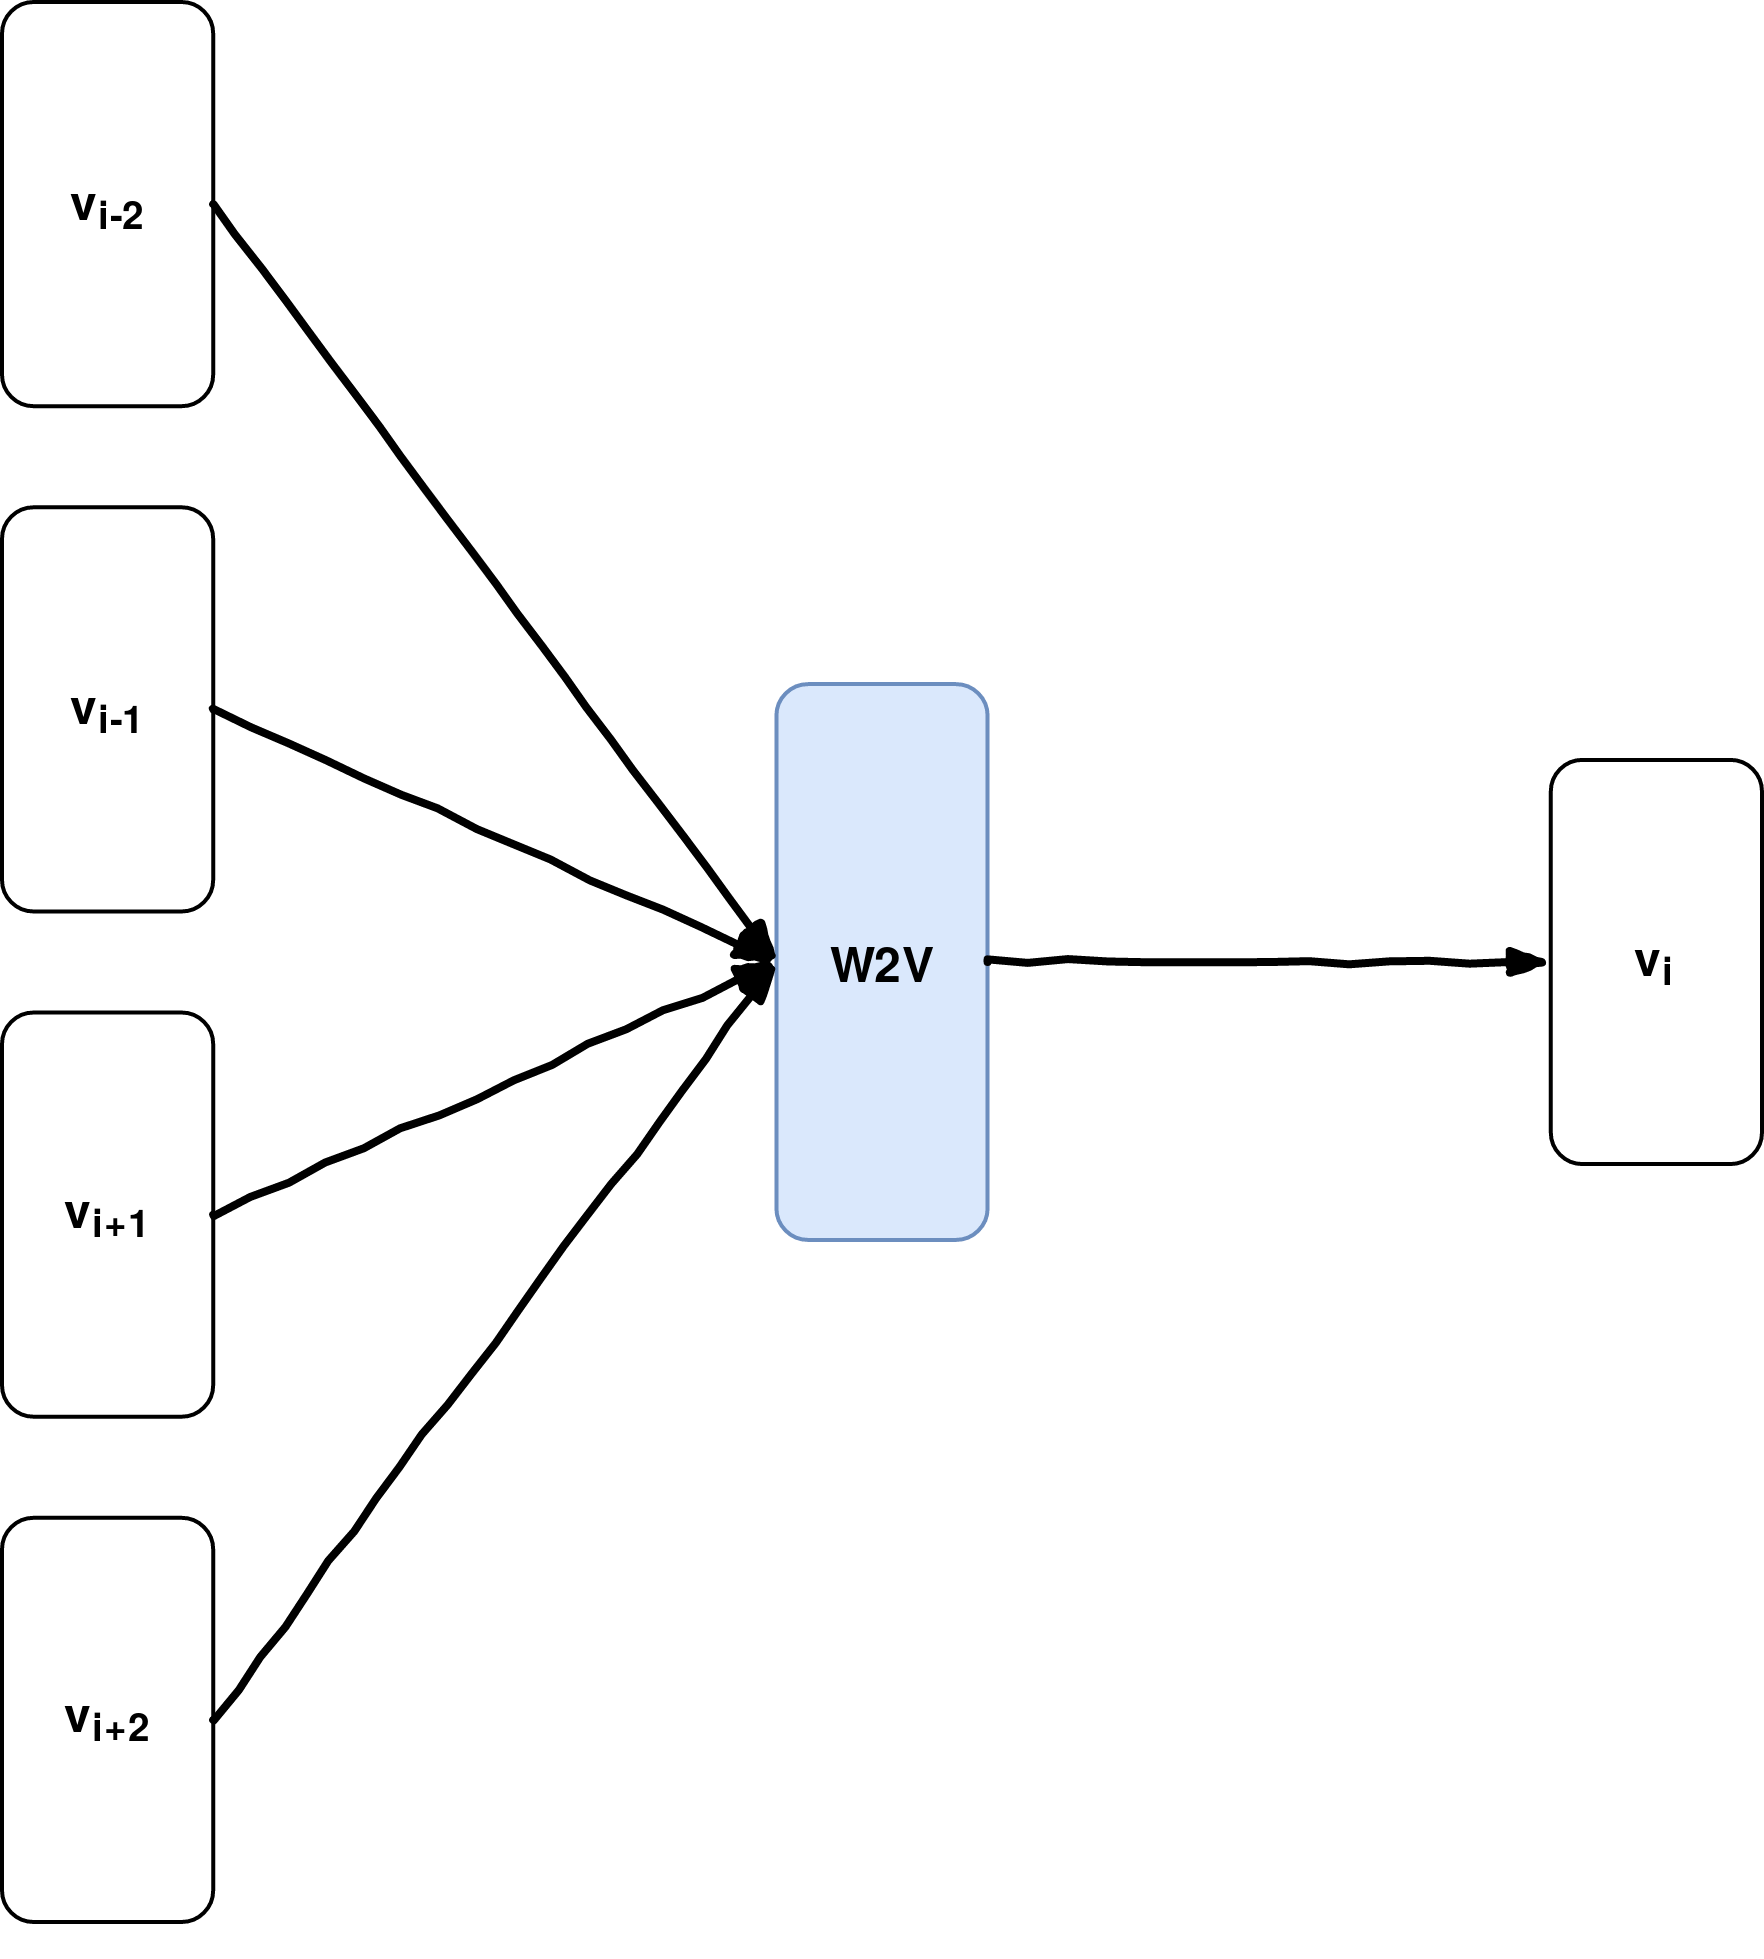
\includegraphics[width=0.5\textwidth,height=150px]{cbow}
	\caption{CBOW modell}
\end{figure}

Skip-Gram modell esetén pont az ellenkezője történik. A háló bemenete $v_i$
$\left( i \in \left|D\right| \right)$ vektor lesz. A tanítás célja, hogy a háló prediktálja az i. szó k méretű kontextusának one-hot kódolt vektorait ($v_{i-k},...,v_{i-1}, v_{i+1},..., v_{i+k} : k \in \mathbb{N}$), közben a háló a rejtett rétegében megtanulja a Word2Vec reprezentációt.

\begin{figure}[H]
	\centering
	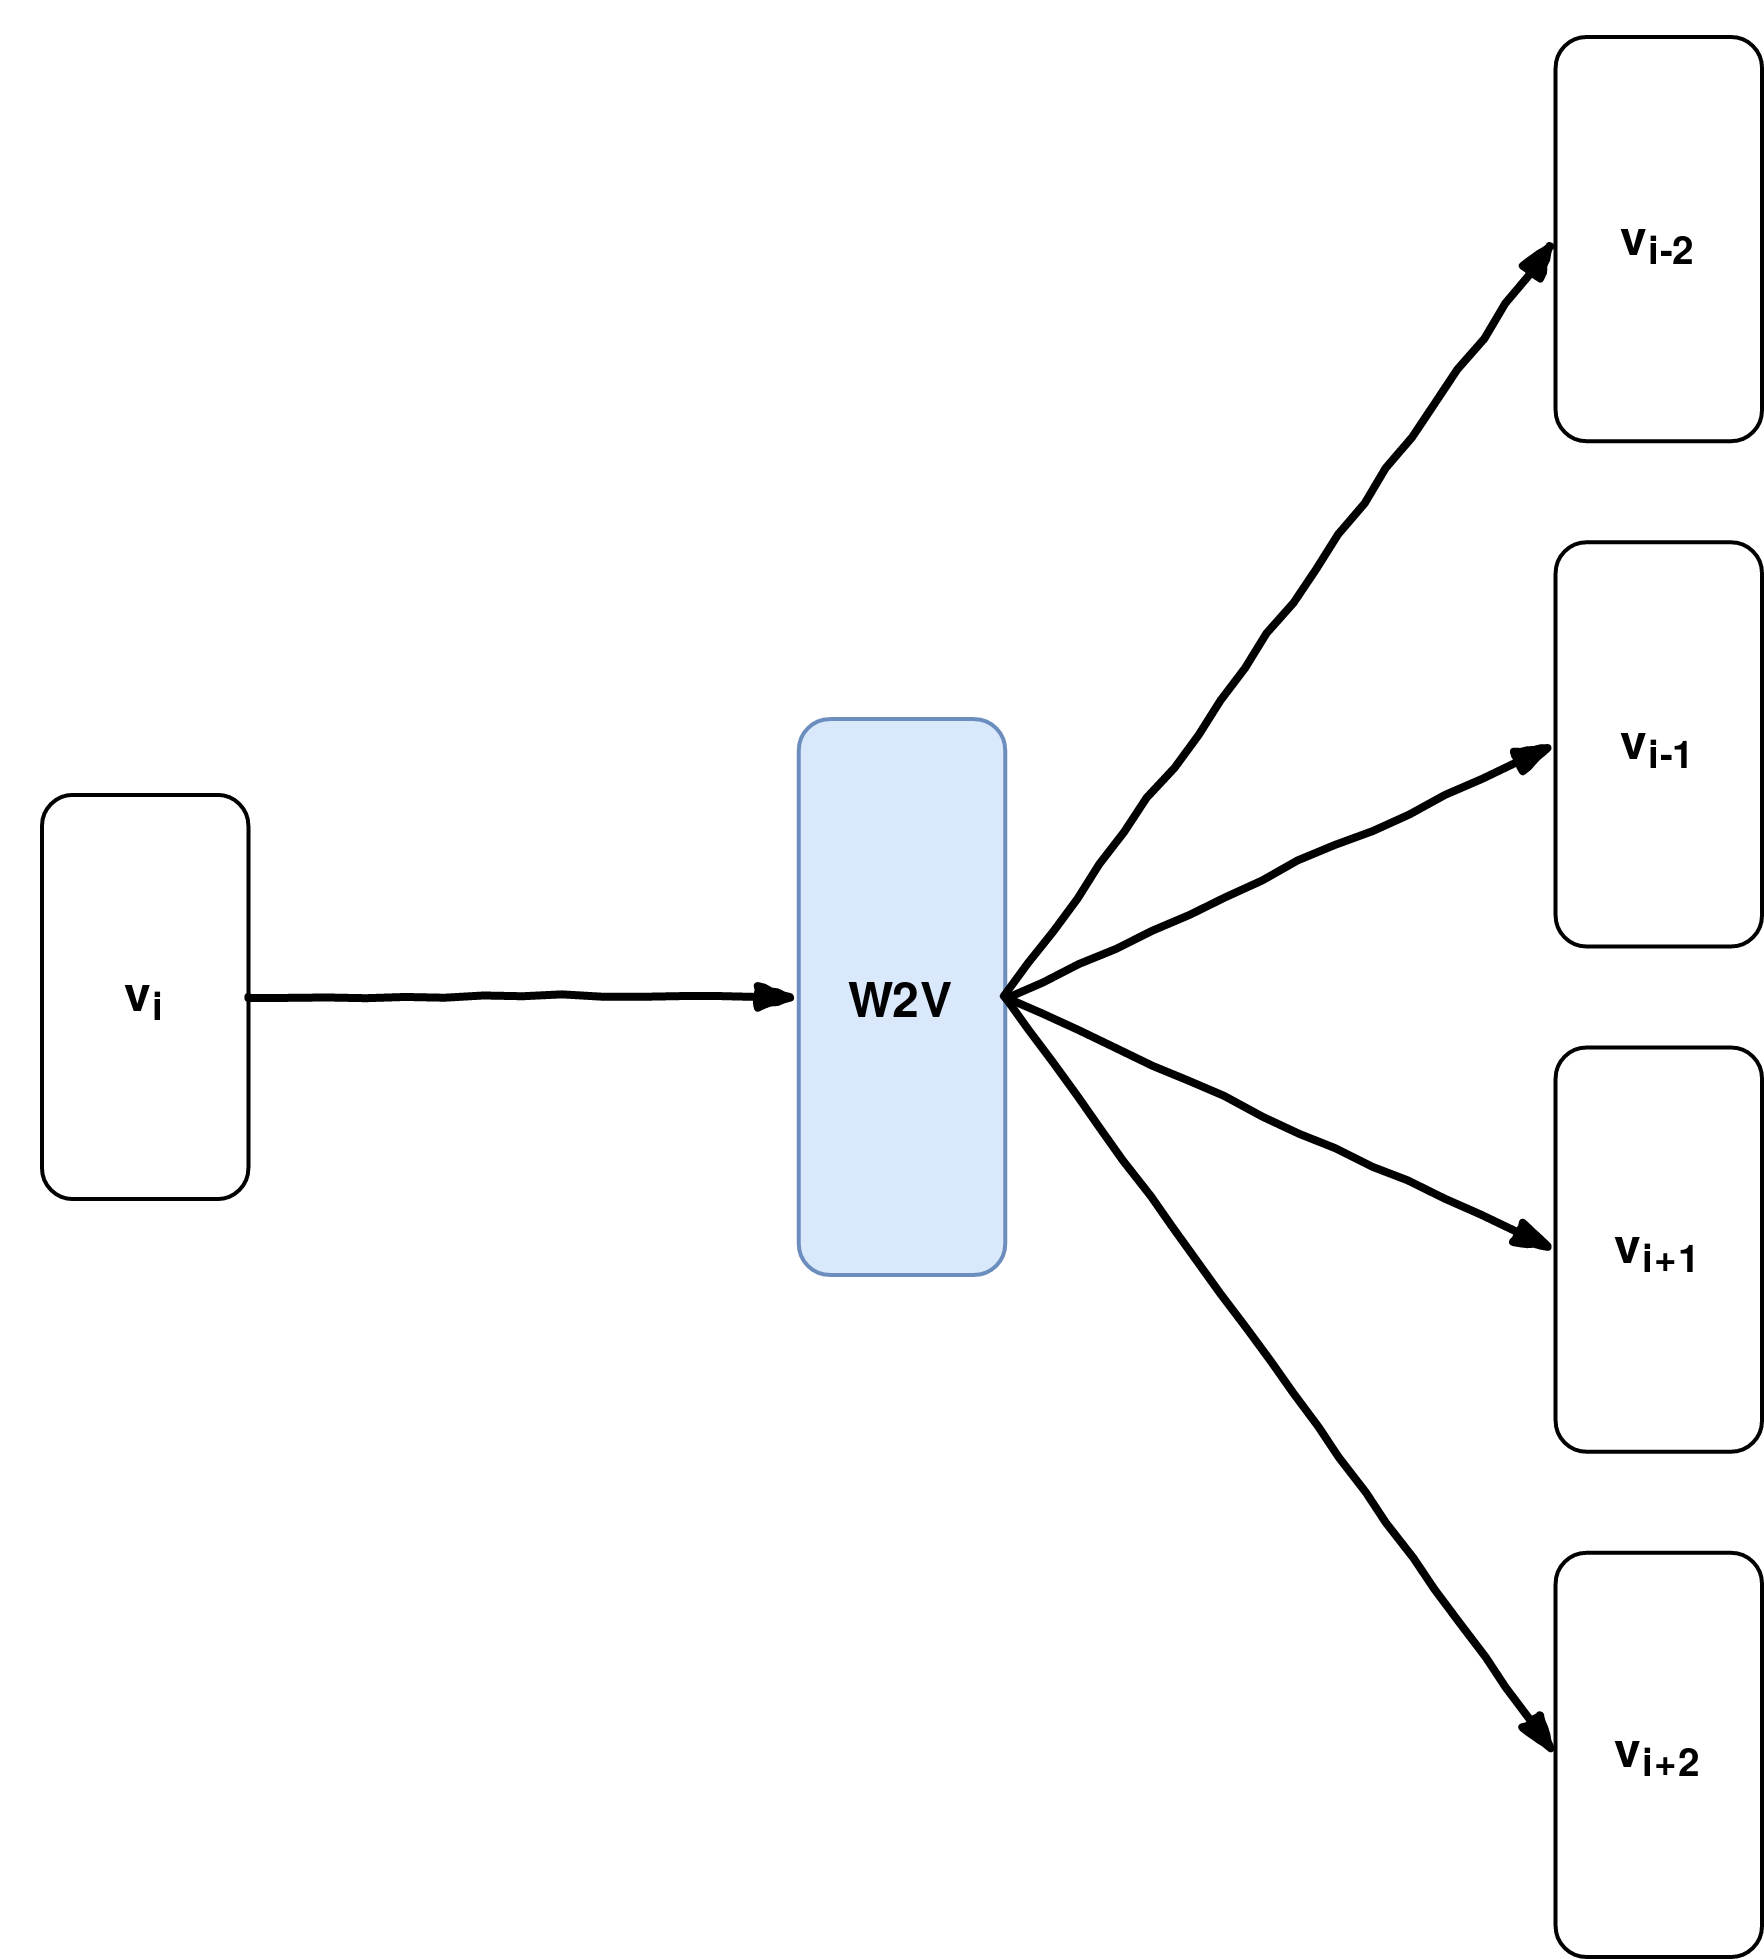
\includegraphics[width=0.5\textwidth,height=150px]{skip-gram}
	\caption{Skip-Gram modell}
\end{figure}

Egy jól tanított Word2Vec modell a hasonló jelentéstartalmú szóvektorokat közel re képezi egymáshoz a vektortérben. 
A teljesítmény növelése érdekében finomhangolhatjuk a tanítási paramétereket. Ilyen beavatkozás lehet ha növeljük a halmaz méretét, amellyel Word2Vec modellünket tanítjuk, vagy emeljük a kontextus ablak méretét és a reprezentációs dimenziót.

\begin{note}
	A Skip-Gram modell a ritka szavak, míg a CBOW modell a gyakori szavak esetén készít pontosabb reprezentációt.
\end{note}


\subsubsection{GloVe}
A Word2Vec bemutatását követő évben újabb nagy lépés történt a szóbeágyazás világában, a \textit{Stanford University} NLP kutatócsoportja publikálta a GloVe módszert.

A GloVe (\textit{Global Vectors}) \cite{pennington2014glove} reprezentációs módszer a Word2Vec-hez képest egy korpusz lokális statisztkáján kívül a globális statisztikáit is figyelembe veszi. 

\begin{definition}
	Adott egy korpusz, melynek elemszáma V. Az $X \in \mathbb{N}^{V \times V}$ mátrixot közös előfordulási mátrixnak nevezzük, ahol $X_{ij}$ az a szám, ahányszor i. szó kontextusában j. szó megjelenik.  
\end{definition}

A GloVe modell tanítása egy korpusz közös előfordulási mátrixának nemnulla elemein történik. A GloVe modell egy log-bilineáris modell, amely feladata, hogy kiszámítsa a következő szó valószínűségét azon kontextusa alapján.

A módszer mögötti intuíció az, hogy a közös előfordulási valószínűségek hányadosa értékes információval szolgálhat a leképezés során. Így a feladat célja, hogy a tanult szóvektorok skaláris szorzata megegyezzen a szavak közös előfordulási valószínűségének logaritmusával. Mivel $\log \left( \frac{A}{B} \right) = \log \left( A \right) - \log \left( B \right)$, így ez a cél összekapcsolja az előfordulási valószínűségek arányszámát a vektorok távolságával.

Ugyan a globális statisztikáknak köszönhetően a GloVe több feladatban is túlteljesíti a Word2Vec-et, a tanításához szükséges közös előfordulási mátrix memóriaigénye magas. Paraméterhangolás esetén újból fel kell építenie a mátrixot, mely költséges művelet.

\subsubsection{ELMo}
A Word2Vec és a GloVe már képes szemantikus információ leképezésére, azonban esetükben az ellentétes szópárok közel kerülnek egymáshoz. Azon feladatoknál, melyeknél az ellentétes szavak kiemelt szerepűek – például a hangulatelemzés – limitációk jelentkezhetnek, továbbá ezen algoritmusok rosszul kezelik az ismeretlen szavakat is.

Míg a Word2Vec és a GloVe csak szavankénti kontextusfüggetlen reprezentáció tanulására képes – azaz nem számít az adott szó környezete, melyre alkalmazzák –, addig az Embeddings from Language Models (ELMo) \cite{elmo} figyelembe veszi a lexémák kontextusát, mondaton belüli elhelyezkedését is. Az ELMo használat közben állítja elő a vektorokat.

A modell tanításához használt neurális háló több réteg kétirányú LSTM (biLSTM) konkatenációja. A különböző rétegek más és más típusú információt képesek eltárolni.

\begin{figure}[H]
	\centering
	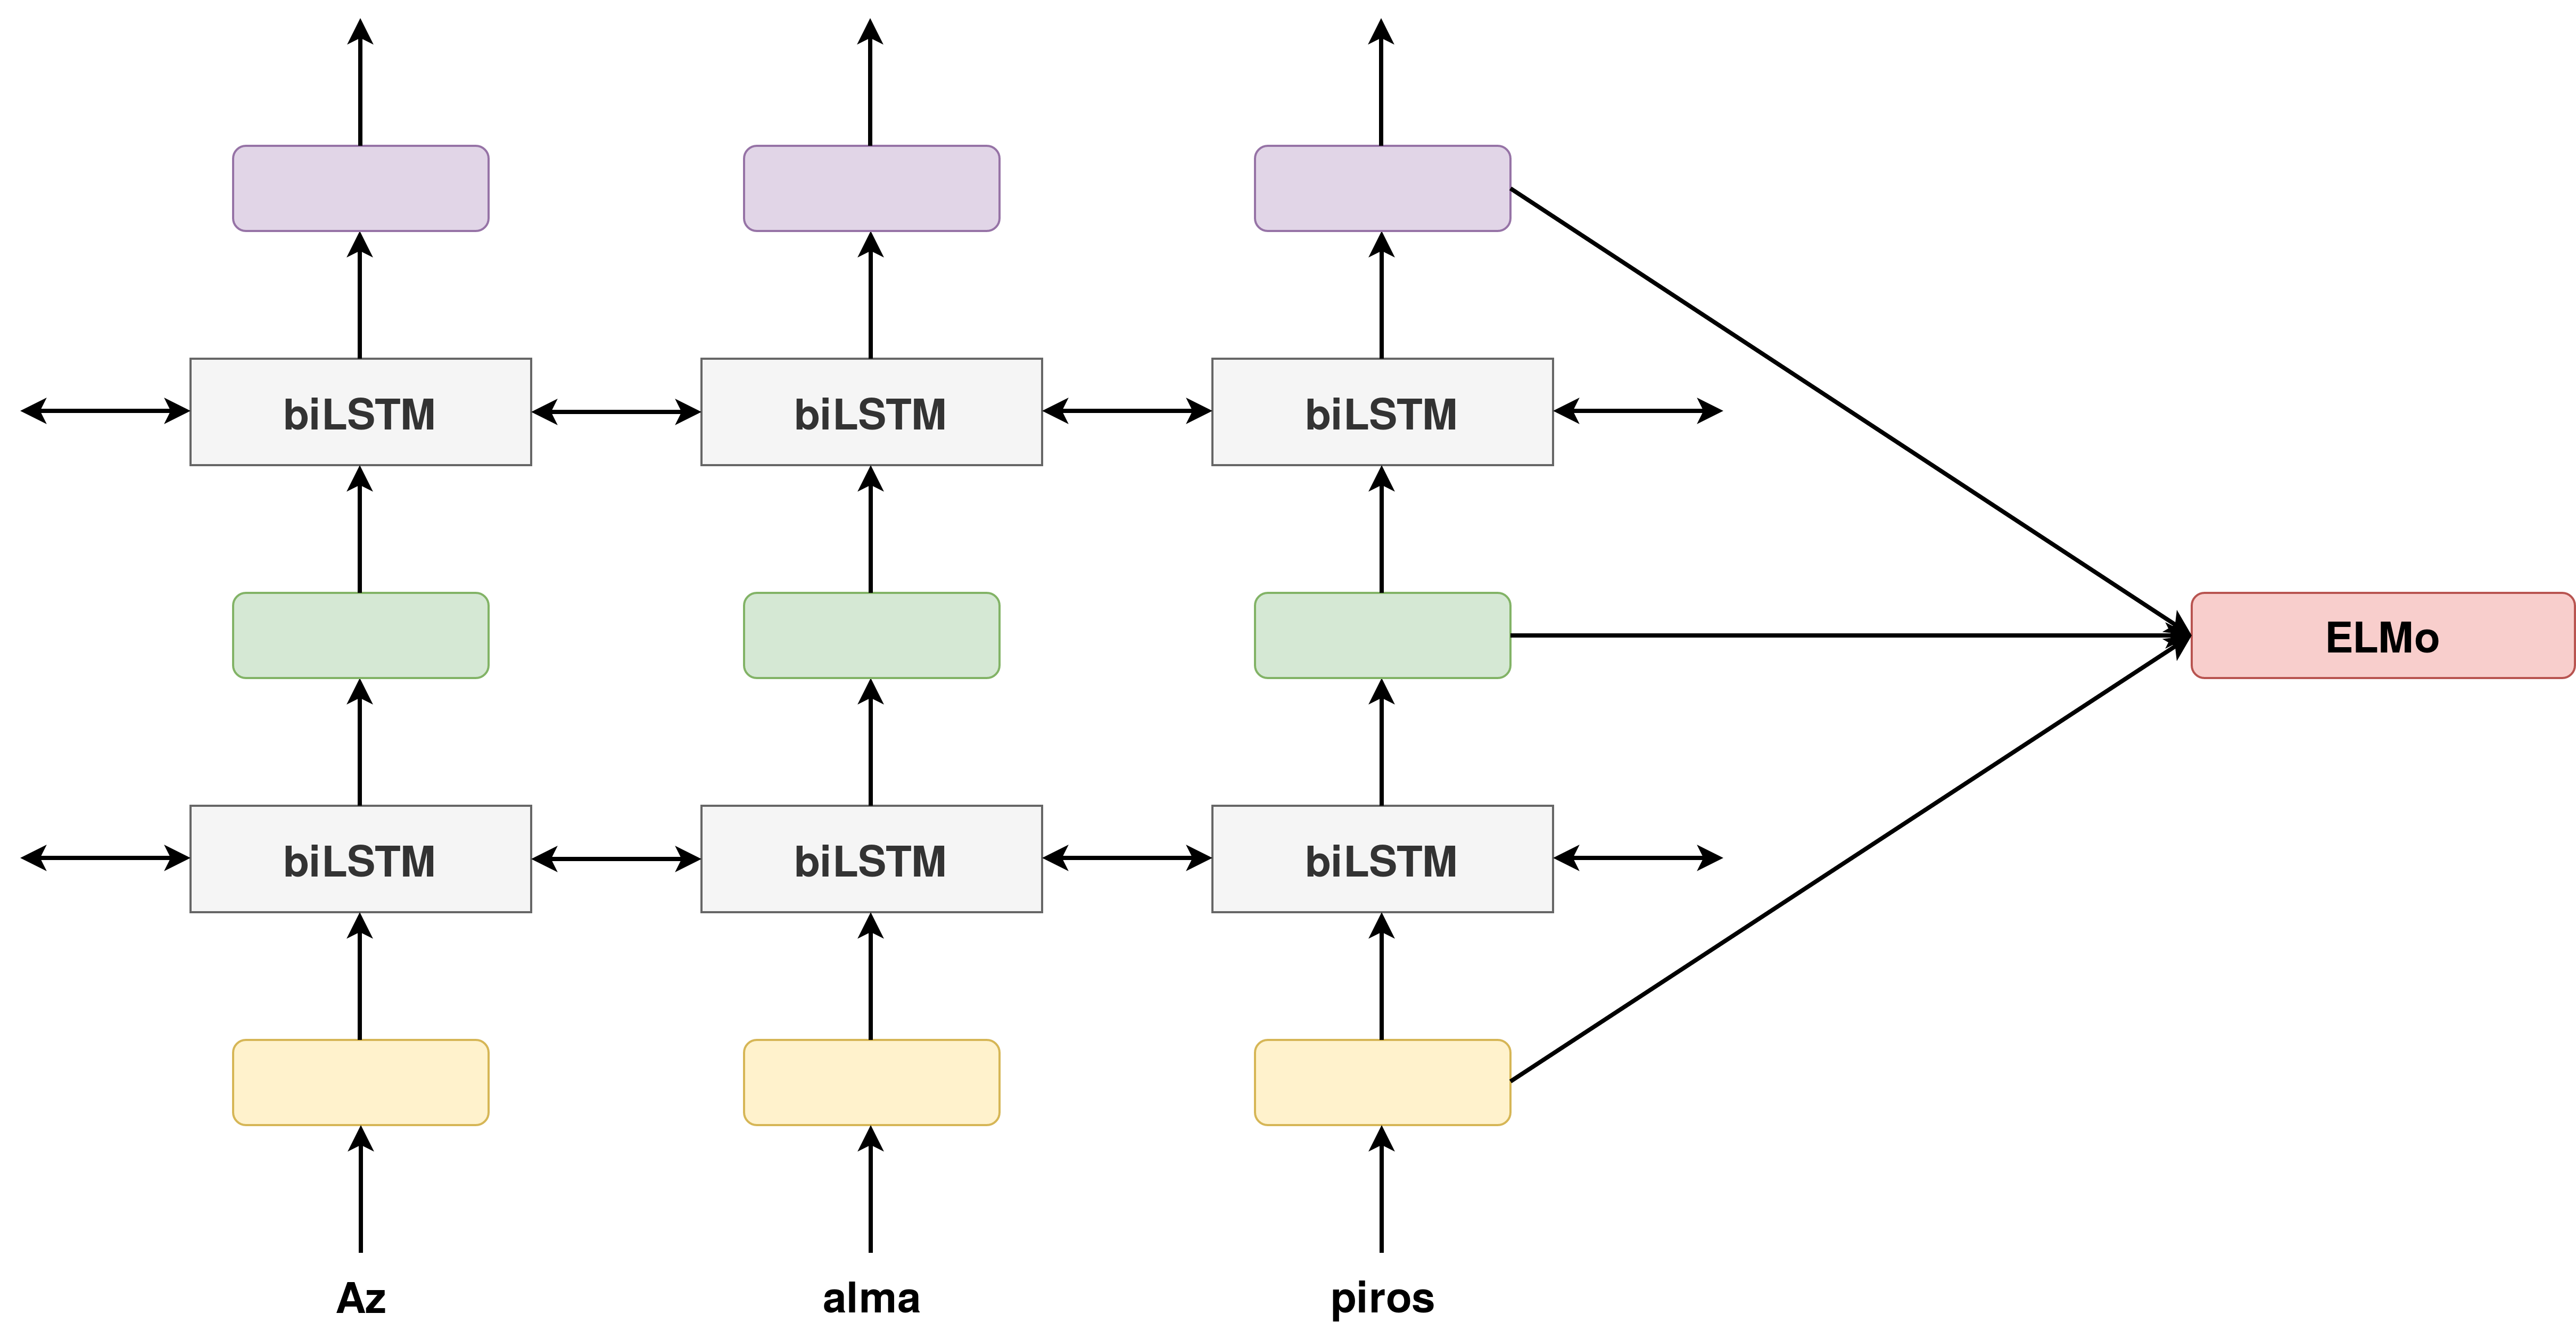
\includegraphics[width=0.8\textwidth,height=200px]{ELMo}
	\caption{ELMo modell}
\end{figure}

Az ELMo a különböző rétegek kimenetének feladatspecifikus kombinációján alapszik. Egy adott NLP feladatra minden BiLSTM réteg egyedi súlyt kap. A végső háló 2 darab BiLSTM rétegből áll, minden LSTM réteg 4096 széles.

Az így kapott sekély kétirányú módszer jelentősen javított a szóvektorok pontosságán.

Bár az ELMo egy karakter (konkatenáció) alapú reprezentációs algoritmus, szavakat ábrázol. Ezen tulajdonsága alapján képes kezelni az addig nem látott szavak problémáját is.


\subsubsection{BERT}
Egy 2018-ban publikált cikk \cite{char} rámutatott arra, hogy a karakteralapú algoritmusok nem teljesítenek olyan jól, mint a szóalapú társaik. A Bidirectional Encoder Representations from Transformers (BERT) \cite{2018arXiv181004805D} egy a Google által kifejlesztett transformer architektúrájú nyelvi modell. Az ELMo-hoz hasonlóan ez is kétirányú, azaz egy szó mindkét oldali kontextusát figyelembe veszi a tanulás alatt. A BERT azonban bemenetként nem szavakat és nem is karaktereket kap, hanem szótöredékeket.

A tanítást a \textit{transfer learning} szerint két fázisra bontották: előtanítás és finomhangolás. 

Az előtanítás két feladatból állt: \textit{következő mondat} és \textit{maszkolás}.
A bemenetben megadták a szótöredék token-eket, a token-ekhez tartozó mondaton belüli helyadatokat és azt, hogy az adott token A vagy B mondat közül melyikhez tartozik.

\begin{figure}[H]
	\centering
	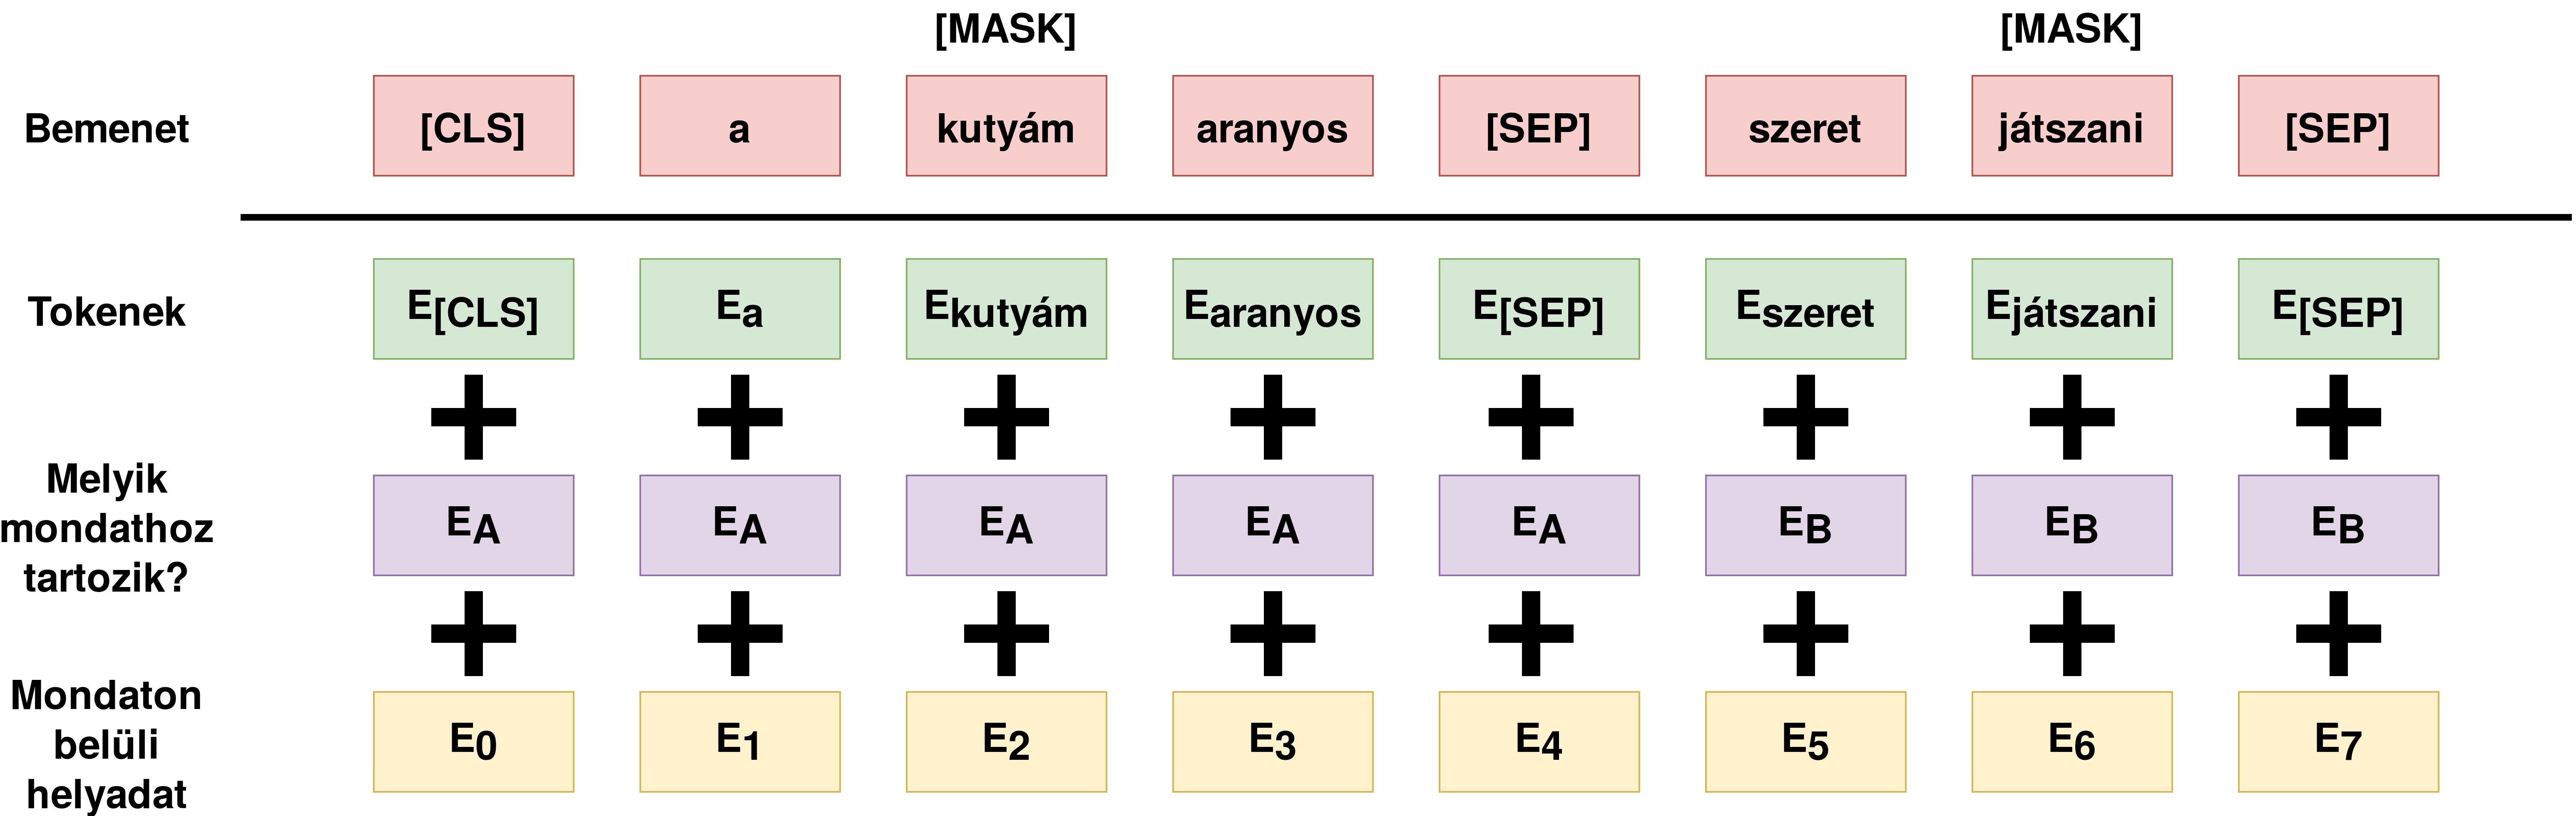
\includegraphics[width=1\textwidth,height=180px]{BERT}
	\caption{A BERT bemenete}
\end{figure}

 A \textit{következő mondat} esetében a mélyháló feladata kitalálni, hogy A[SEP]B input mondatokra B rákövetkezője-e A-nak. A \textit{maszkolás} során véletlenszerűen letakarták a token-eket a mondatokban és a mélyháló megpróbálta kitalálni, hogy eredetileg melyik szó volt a [MASK] token helyén.  A [CLS] token a klasszifikációs feladat alatt a mondatot ábrázolja, a [SEP] a mondatok közötti szeparátor és a [MASK] a letakart szótöredékeket helyettesíti.

A továbbiakban a modell finomhangolása az adott NLP feladat szerint történik.

Míg az ELMo különböző balról-jobbra és jobbról-balra olvasó rétegek konkatenációjaként állítja elő a vektorokat, addig a BERT a valódi mély architektúrájával csak egyszer dolgozza fel a token-eket. A \textit{transformer} architektúra nem igényel vektoriális bemenetet, saját reprezentációt épít a token-ek számára is.

A BERT szótöredék alapú megoldása egyesíti a karakteralapú modellek előnyét a szóalapú modellek előnyével. Képes kezelni az ismeretlen szavakat és performanciája mégis magas marad. A \textit{következő mondat} feladat a szövegben található mondatok közötti relációk, a \textit{maszkolás} pedig a mondatokon belüli szemantikai és szintaktikai információ ábrázolását segíti. Több NLP feladat megoldásában is jelenleg a BERT a \textit{State-of-the-art}.

\section{Reprezentáció a mondatok és magasabb nyelvi elemek szintjén}

Ahogy a lexémák szemantikai tartalmát sem határozza meg az őket alkotó karakterek lánca, úgy a mondatok sem értelmezhetőek pusztán a magukban foglalt szavak halmaza alapján. A mondatok és magasabb nyelvi elemek interpretálása során fontos tényezők lehetnek a bennük lévő szintaktikai viszonyok és a kontextus is.

Néhány NLP feladatnál, mint például a dokumentumok szemantikus keresésénél, vagy szöveg összegzésnél szükség lehet magasabb szintű reprezentációkra.  Ezek a módszerek szavak helyett mondatokat, bekezdéseket, vagy akár egész dokumentumokat tesznek numerikusan értelmezhetővé. 

\subsection{Mondatvektorok}
A szóvektorokhoz hasonlóan úgy kaphatunk mondatvektorokat, ha mondatokat helyezünk el egy vektortérbe. A tanítás során azonban a sorrendiség, az egyes lexémák változó súlya és a szintaktikai viszonyok megnehezíthetik dolgunkat. Szükség van egy technikára, mely segítségével leképezhetjük és szemantikai tartalmuknál fogva összegezhetjük a megfelelő rendezett szóvektorok sorozatát, így hozzájutva az adott mondat reprezentációjához. A módszerünk akkor hatékony, ha az azonos jelentéstartalmú mondatvektorok klaszterekbe tömörülnek a vektortérben.

\subsubsection{Skip-thought vektorok}
A Skip-though \cite{skip} egy 2015-ben bemutatott mondatreprezentációs módszer – a Skip-Gram algoritmus kiterjesztése – , amely a környező mondatokat is figyelembe veszi a tanulás során. 

A szerzők rekurrens enkóder-dekóder architektúrát használtak a tanításhoz. A neurális háló bemenete mondathármasok szavainak Word2Vec vektoraiból állt. A háló feladata $s_i$ mondat esetén $s_{i-1}$ és $s_{i+1}$ mondatok generálása volt.

\begin{figure}[H]
	\centering
	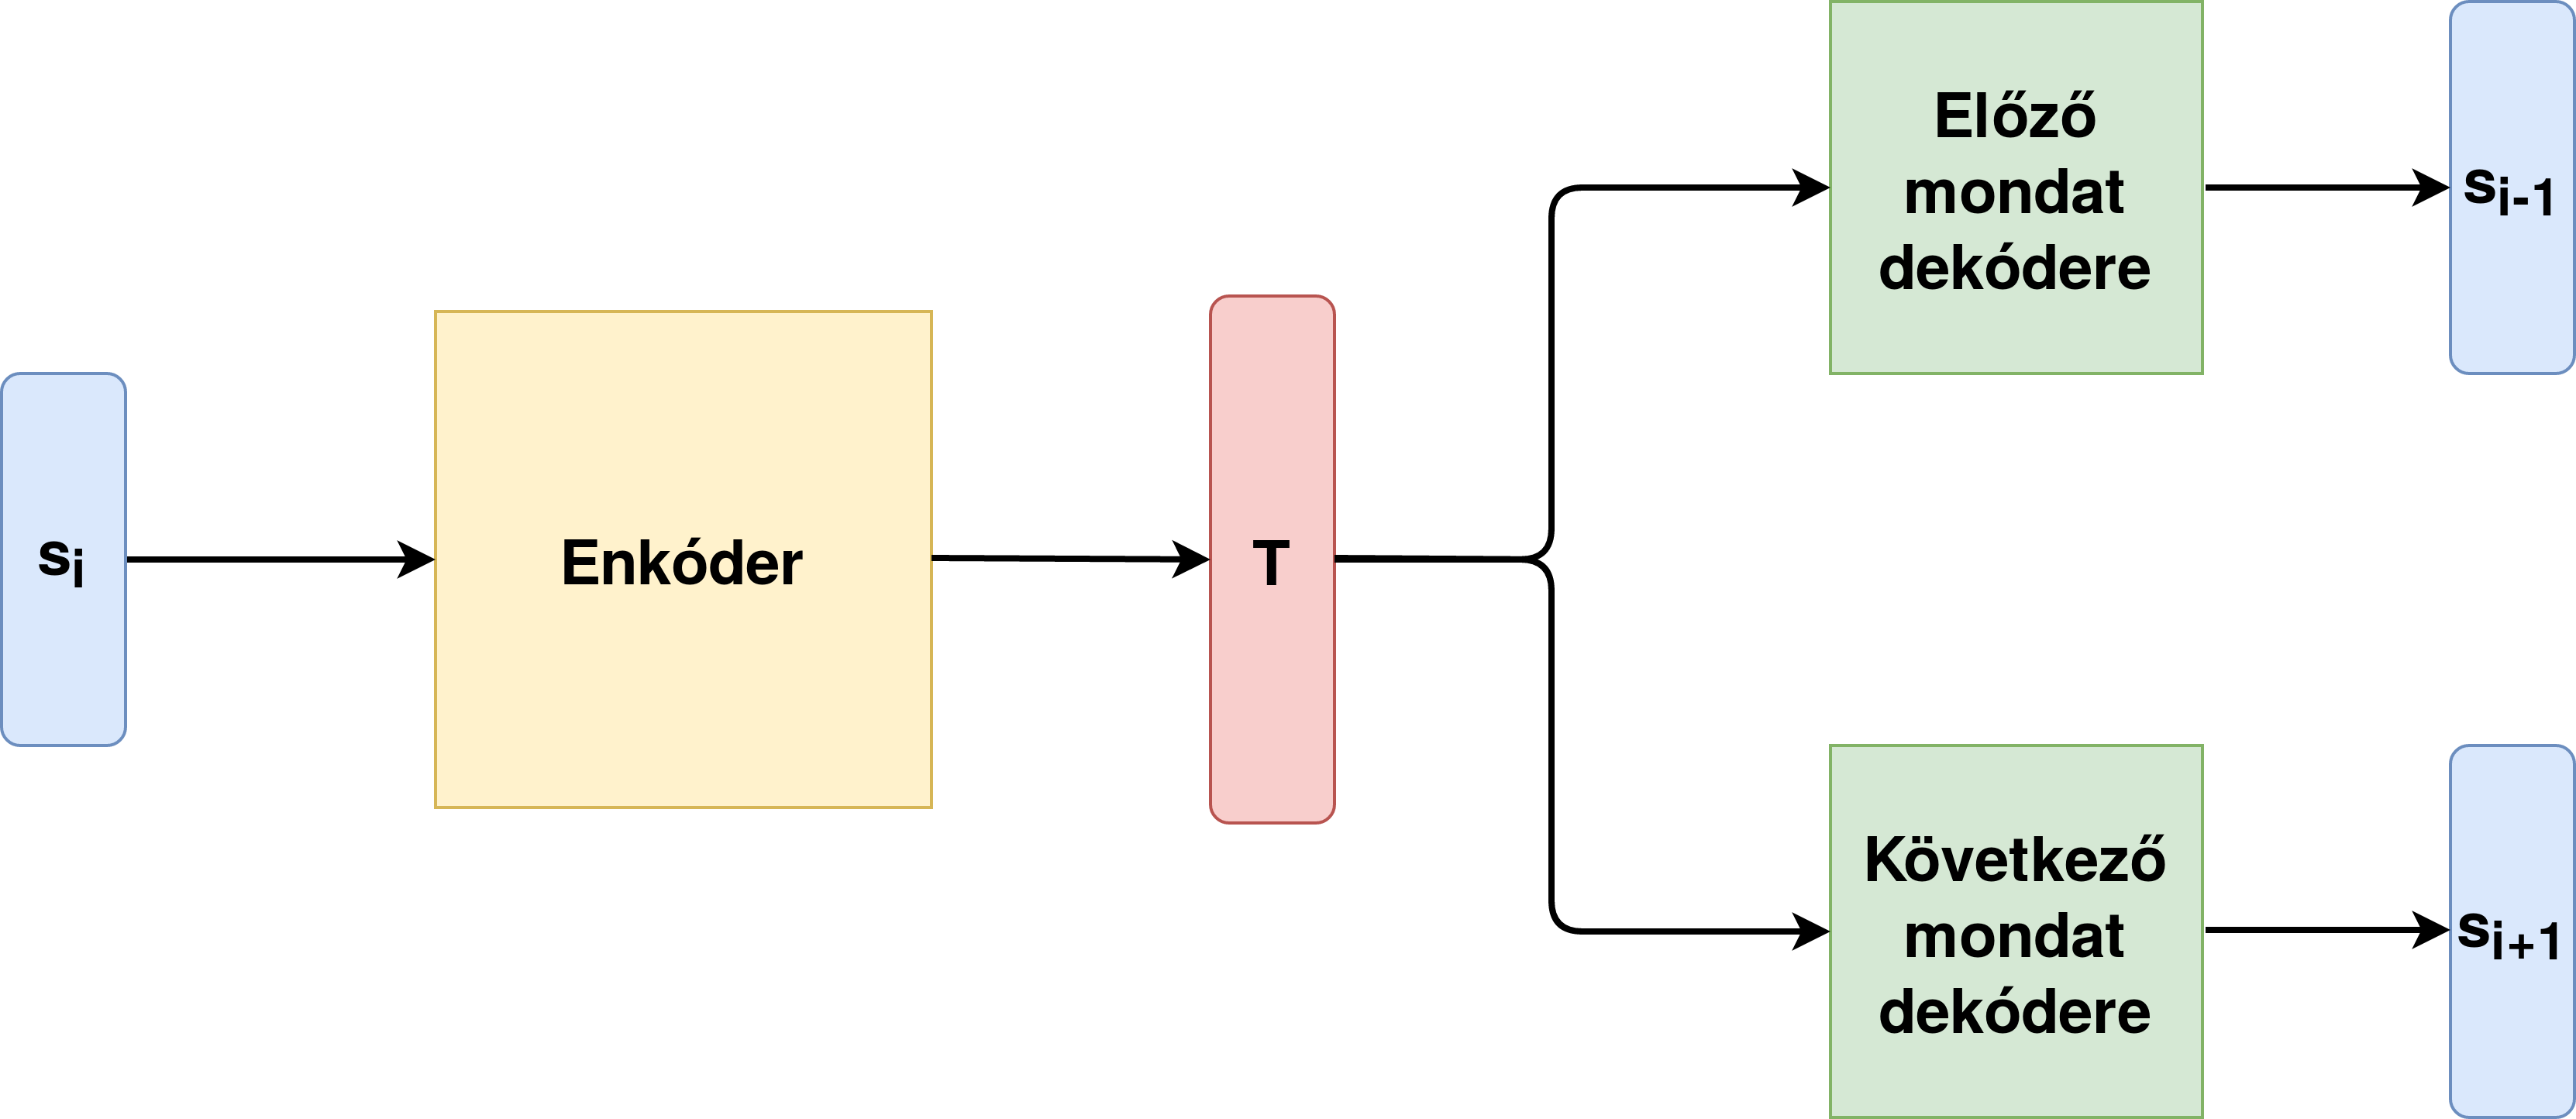
\includegraphics[width=0.6\textwidth,height=130px]{Skip-thought}
	\caption{A Skip-thought enkóder-dekóder architektúrája}
\end{figure}

Az enkóder és dekóder blokkokhoz rekurrens hálót használtak, melyek lehetnek LSTM és GRU rétegek is. Az enkóder célja a legjobb teljesítményével segíteni a dekóder blokkokat, míg a dekóder blokkok célja minimalizálni az előző és a következő mondat rekonstrukciós hibáját.


Olyan szavak esetén, melyeket a háló még nem ismert, tanítottak egy $f:V_{w2v} \rightarrow V_{rnn}$ lineáris leképezést, ahol $V_{w2v}$ és $V_{rnn}$ rendre a Word2Vec és a rekurrens modell szótára. A reprezentáció vektora a rejtett, úgy nevezett \textit{thought} vektor (T).

Bár a \textit{Skip-thought} módszer képes a mondaton belüli és kívüli sorrendiségi információ leképezésére is, csak olyan esetben teljesít megfelelően, ahol az egyes mondatok – melyekre alkalmazzák – megfelelő kontextusban szerepelnek, nem izoláltak.

\subsubsection{InferSent}
2017-ben a Facebook kutatói jelentős áttörést értek el a mondatszintű reprezentációs módszerek terén, a technika neve InferSent \cite{infer}. Hasonló algoritmusokkal ellentétben a szerzők felügyelt tanítást végeztek, melyhez az SNLI adathalmazt vették igénybe. A cikk megmutatta, hogy egy kisebb adathalmazon történő felügyelt tanítás felülmúlhatja a nagyobb adathalmazon nem felügyelt módon tanított modellek teljesítményét.

Az SNLI adathalmaz 570 ezer darab – ember által írt és címkézett – mondatpárból áll. A címkék a következők: következmény, ellentmondás és semleges.

Négyféle neurális architektúrát összemérve a legpontosabb eredményt a BiLSTM + max pooling mutatta. 

\begin{figure}[H]
	\centering
	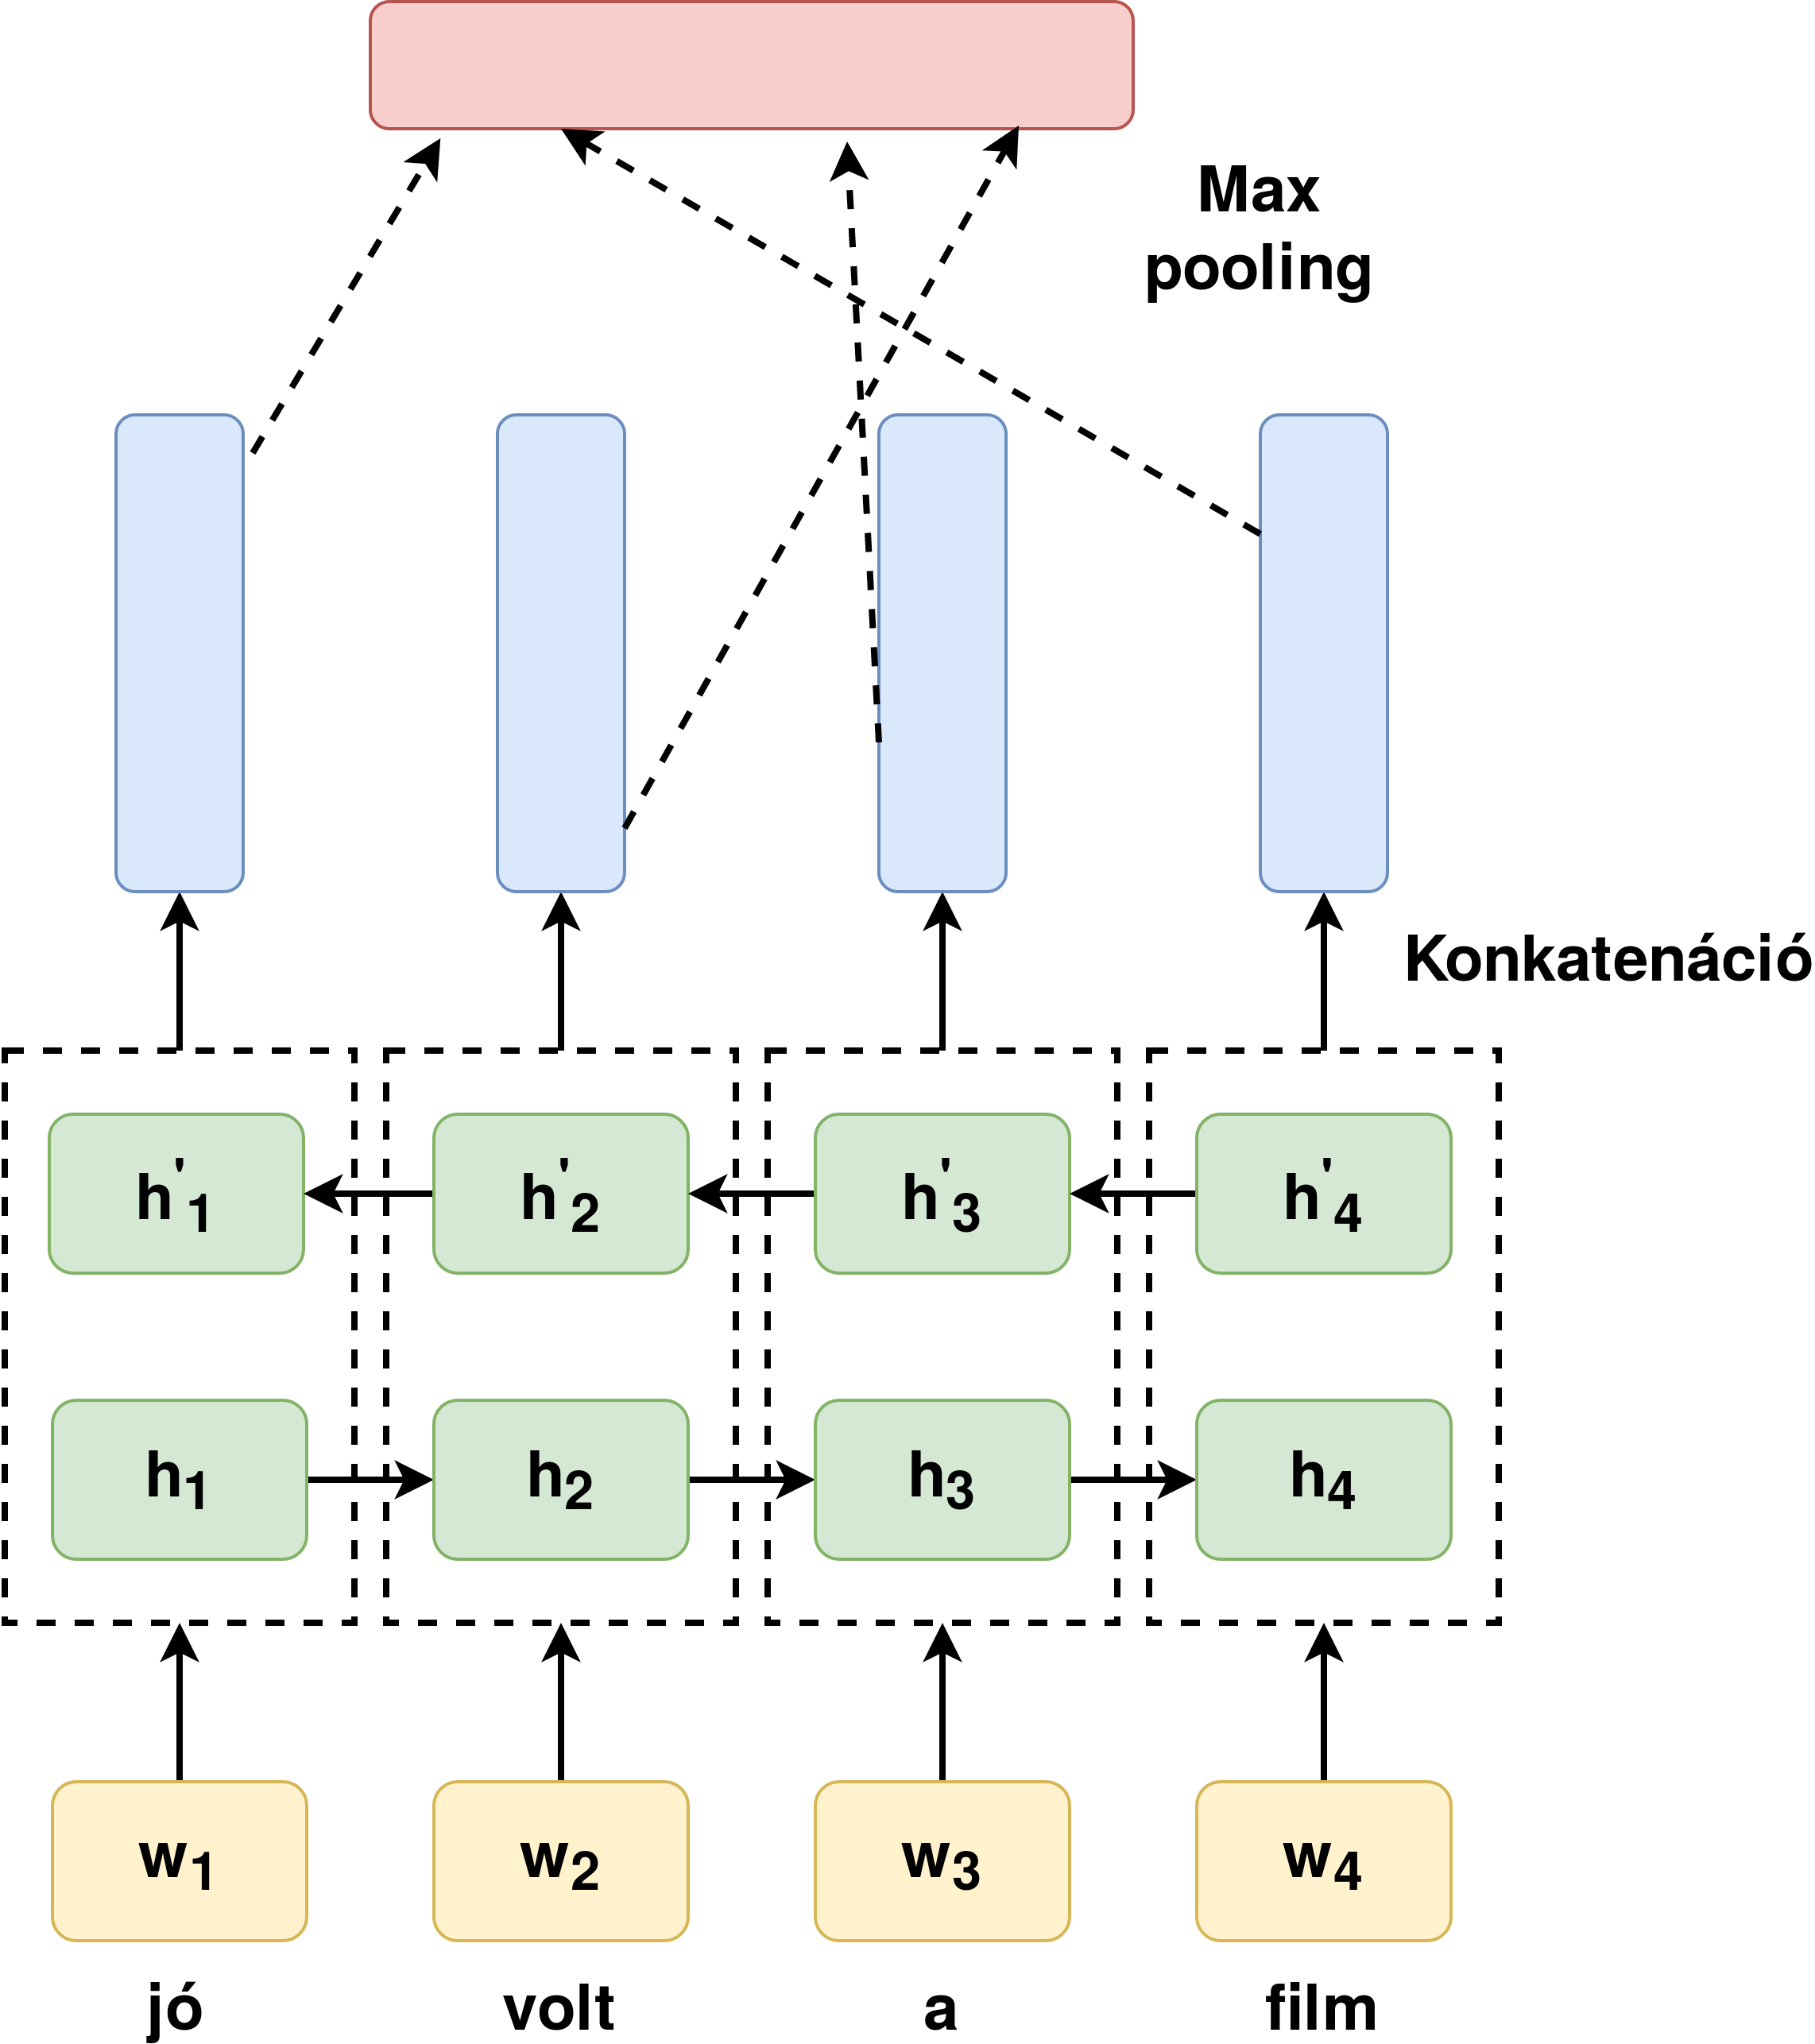
\includegraphics[width=0.5\textwidth,height=200px]{biLSTM-max-pooling}
	\caption{A BiLSTM + max pooling architektúra}
\end{figure}

Az SNLI feldolgozásához szükséges NLI feladat speciális szerkezetet igényel. Mivel kontextusfüggetlen reprezentációt akartak előállítani, amely izolált formában is működik, a mondatpárok GloVe vektorait szeparáltan enkódolták.

\begin{figure}[H]
	\centering
	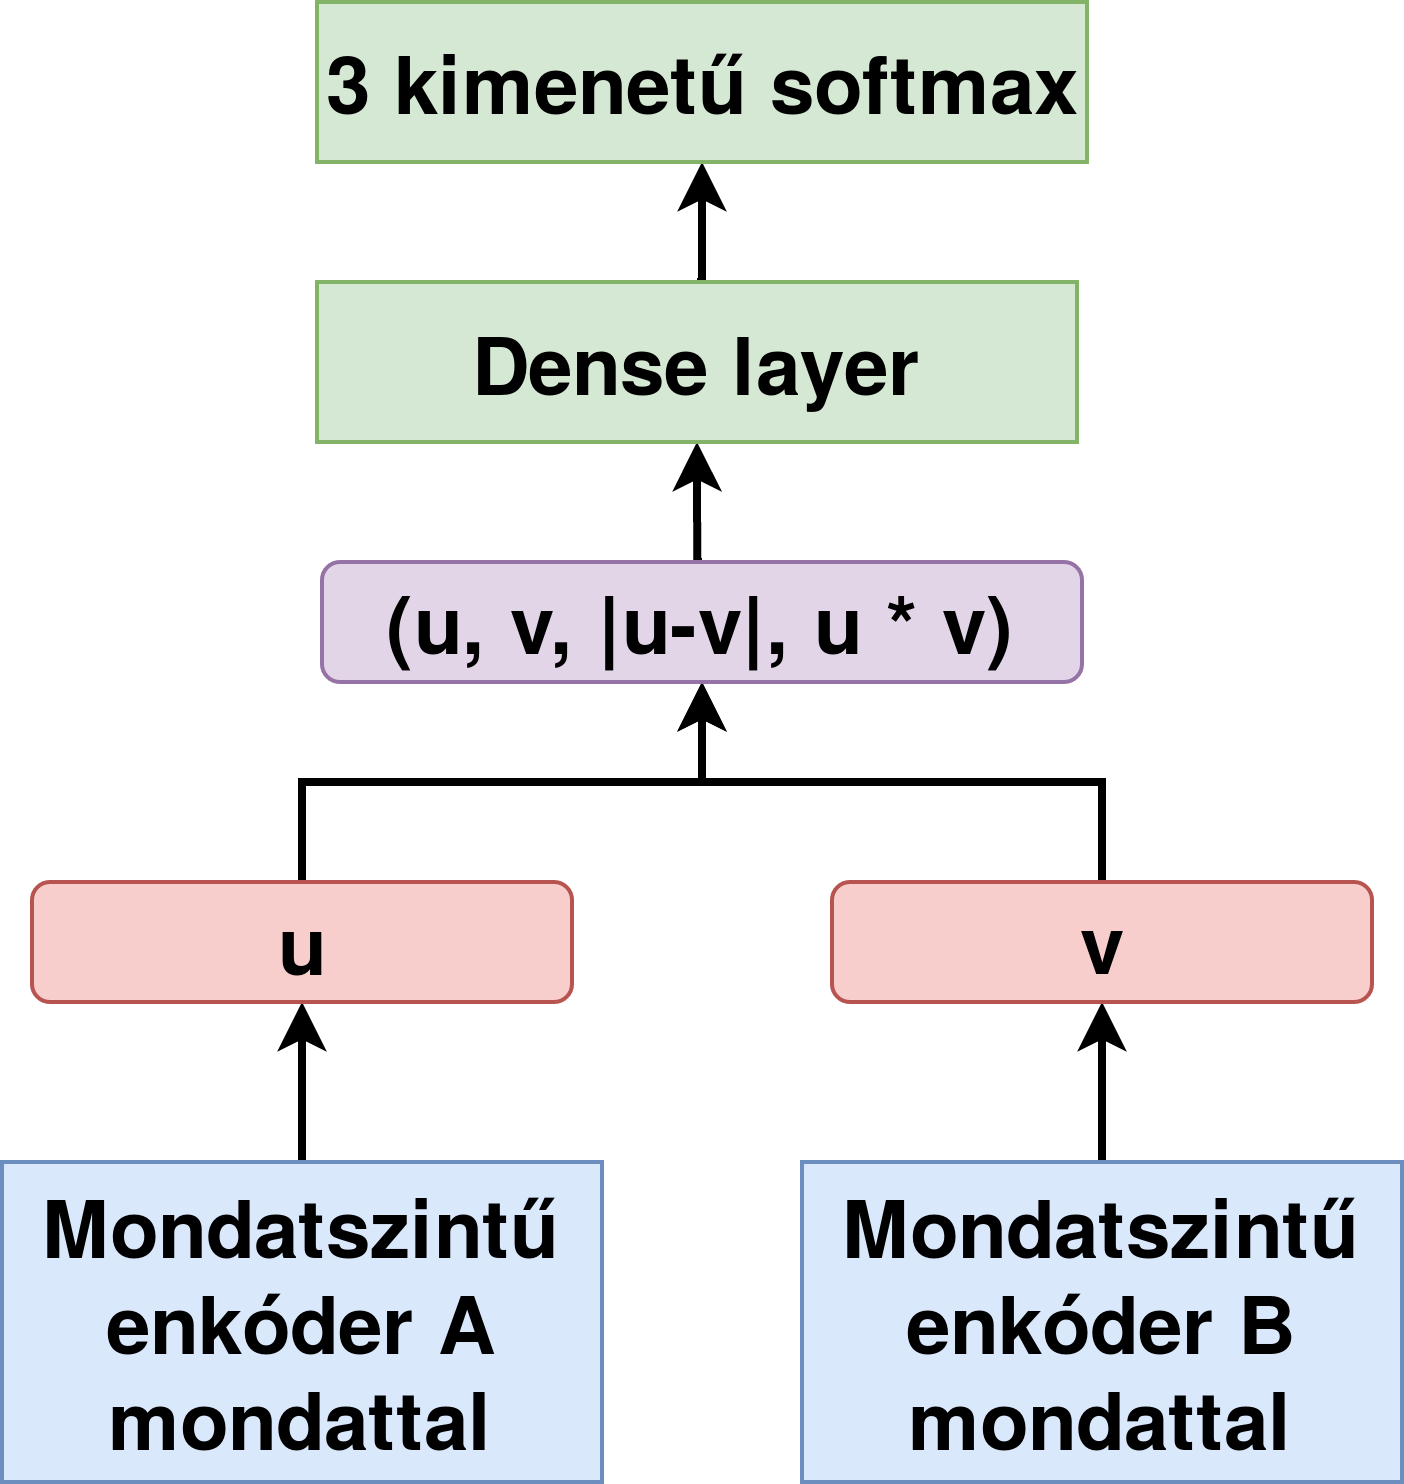
\includegraphics[width=0.5\textwidth,height=150px]{NLI}
	\caption{Az NLI feladat}
\end{figure}

Az így készült u és v vektorokból egy speciális reprezentáció készült: u, v, $\left| u - v \right|$ és $u \ast v$ (vektoriális szorzat) konkatenációjával, melyet végül egy 3 osztályú klasszifikáló hálóba vezettek.

A szerzők a reprezentációs vektorméret növelésével pontosabb eredményt kaptak, de a vektorok memóriaigénye emelkedett. Az InferSent megoldja a kontextusfüggőség problémáját, így a módszer már szövegrészletekre is alkalmazható.

\begin{note}
	Az InferSent napjaink egyik legjobb teljesítményű szemantikus reprezentációs algoritmusa.
\end{note}

\subsubsection{USE}
Az InferSent bemutatását követő évben a Google Research csapata a modern reprezentációs módszereket vizsgálta a \textit{transfer learning} aspektusából. A Universal Sentence Encoder (USE) \cite{use} egy mondatszintű  algoritmus, mely célja, hogy a használója könnyedén igényeire tudja formálni, annak érdekében, hogy pontosabb leképezést kapjon. A szerzők két architektúrát használtak: a BERT-ben említett \textit{transformer}-t és a DAN-t (\textit{Deep Averaging Network}). 

\begin{figure}[H]
	\centering
	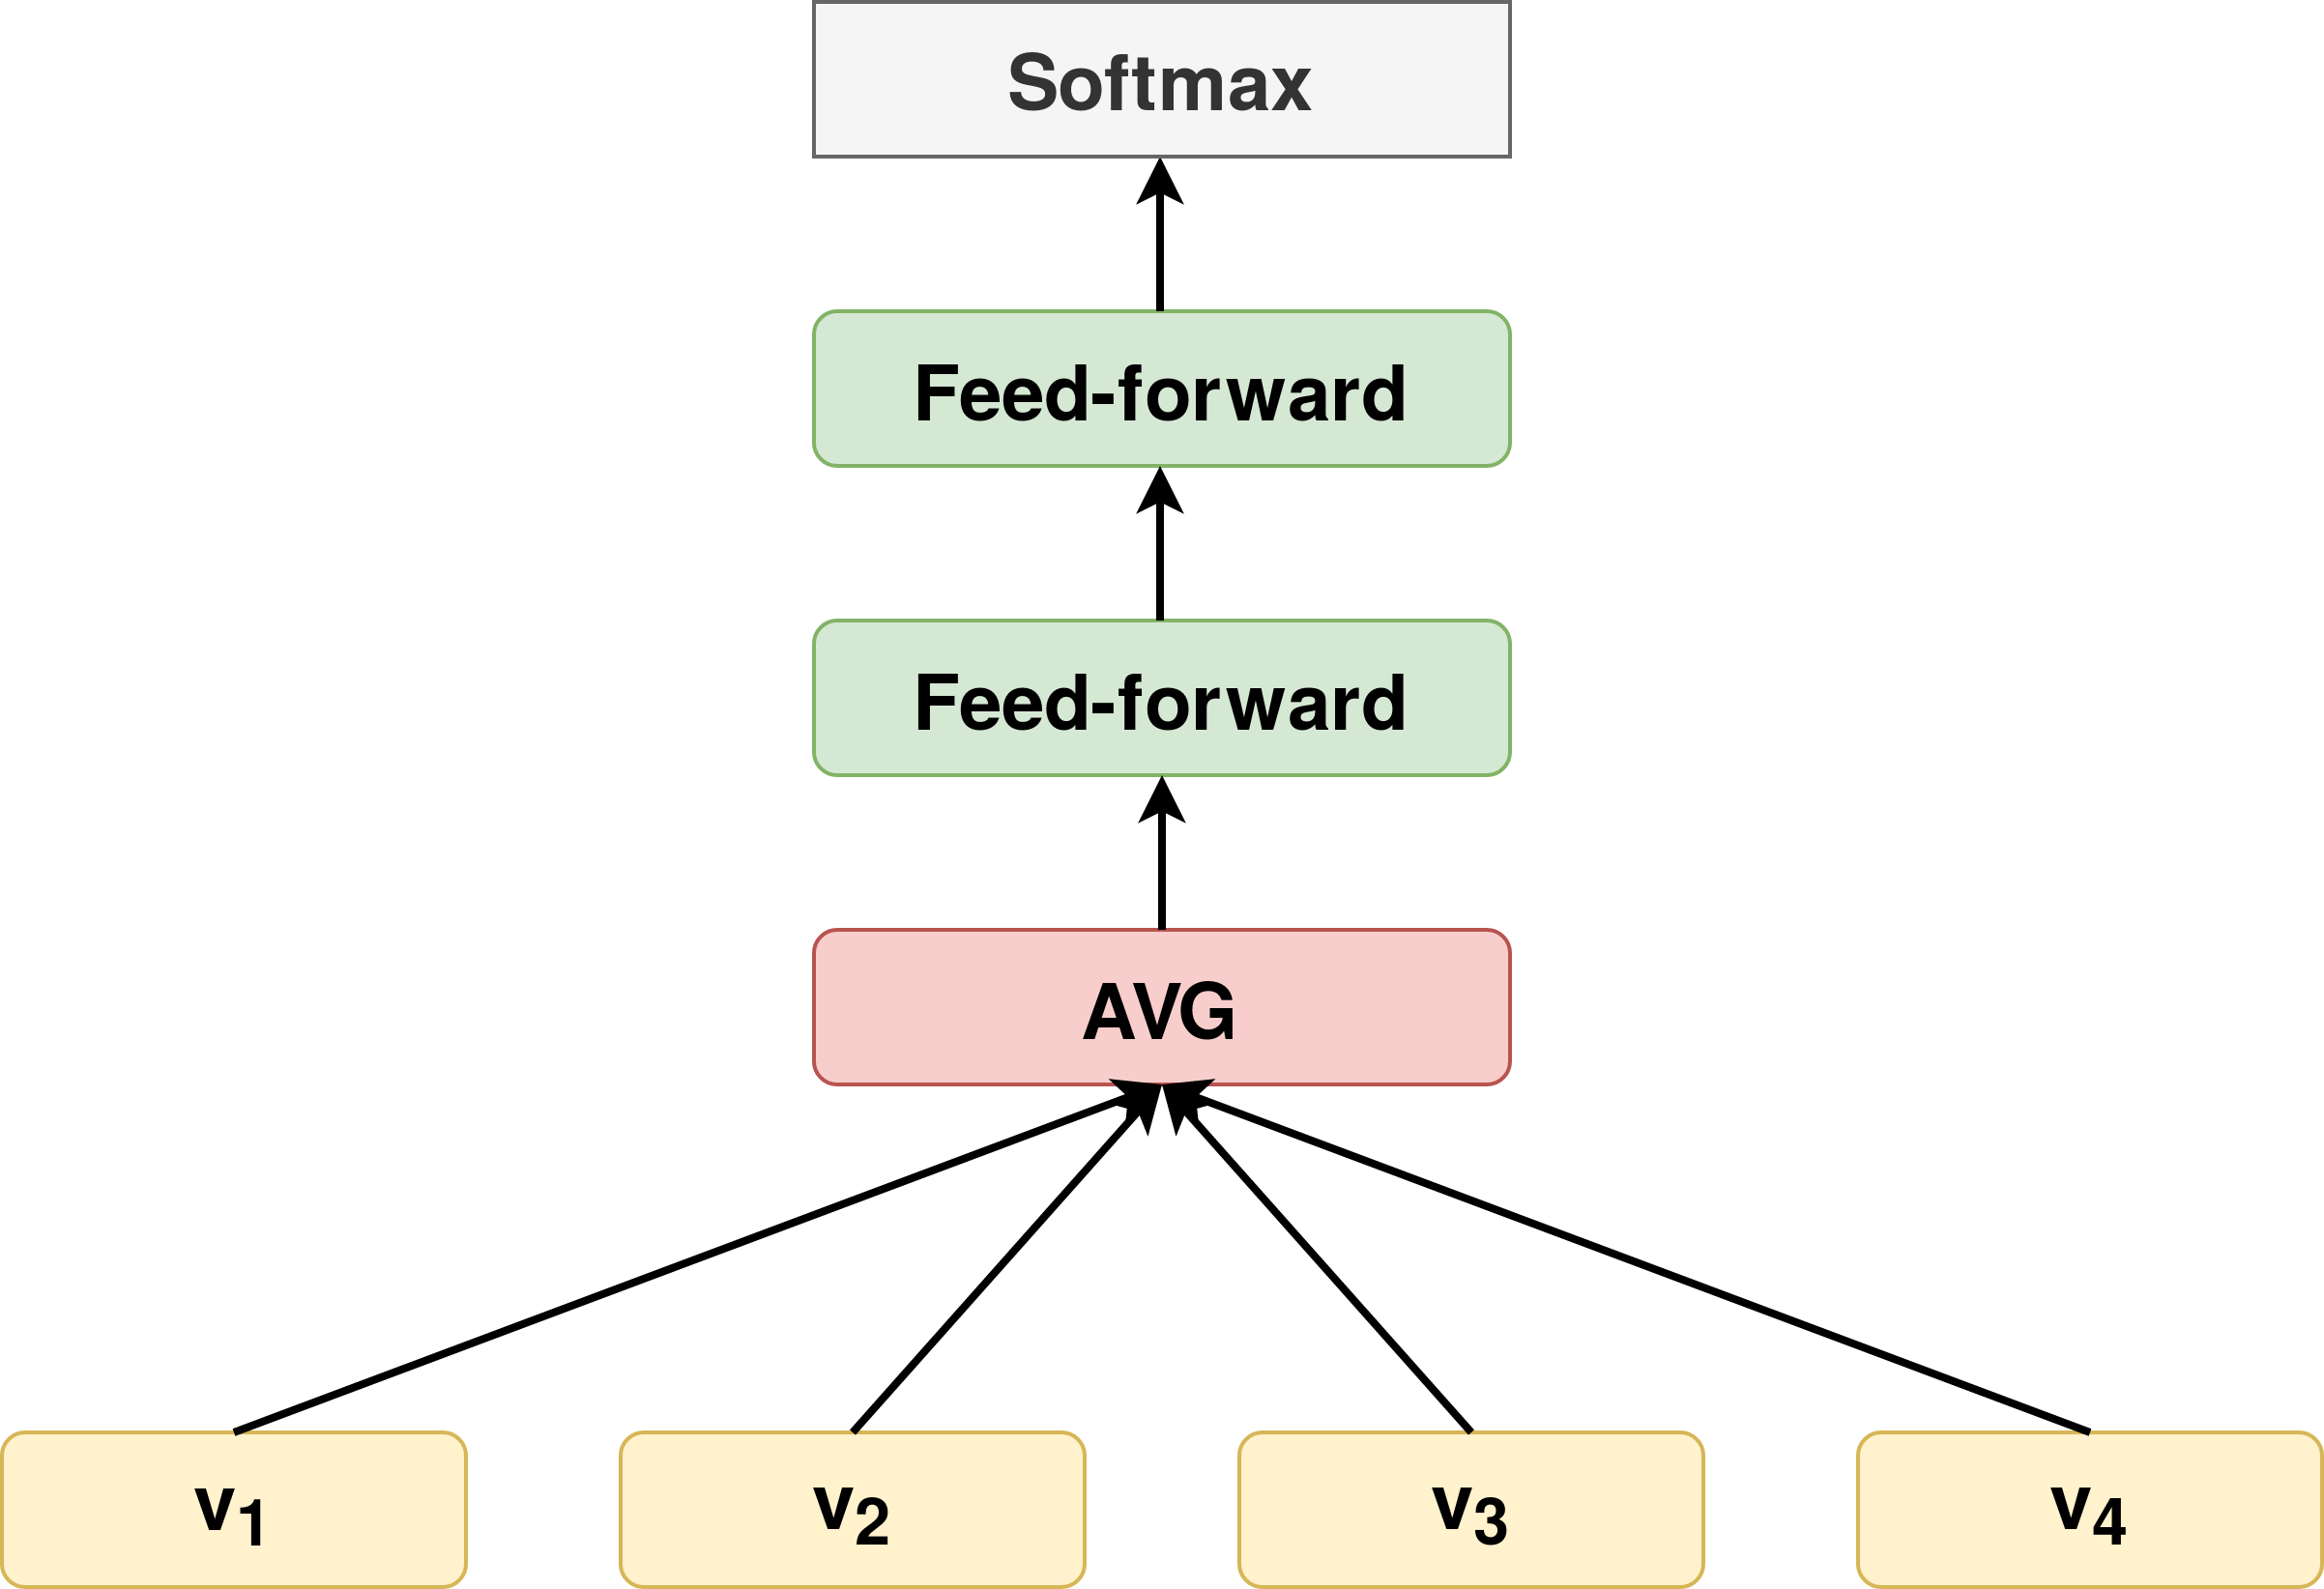
\includegraphics[width=0.6\textwidth,height=150px]{DAN}
	\caption{DAN architektúra}
\end{figure}

A \textit{transformer} modell egyik algráfja a mondatokban lévő szavak kontextusfüggő reprezentációját állítja elő. A folyamat során figyelembe veszi az egyes lexémák sorrendi és egyéni információit is, majd összegzi őket, így megkapja a végső mondatszintű reprezentációt.
A \textit{DAN} modell az input tokenek vektorait először átlagolja, majd \textit{feed forward} rétegek segítségével előállítja a mondatvektorokat. A USE szavakból, mondatokból, vagy akár rövidebb bekezdésekből is képes 512 méretű vektorokat generálni.

A neurális hálók tanítását két részre bontották, bemenetként angol nyelvű karakterláncokat kaptak. Az első rész a \textit{Skip-thought}-hoz hasonló módon, dialógusokból vett mondat-válasz párokkal, illetve felügyelt módon a \textit{Stanford Natural Language Inference} (SNLI) korpuszon történt.

A cikk során kiemelt szerepet kapott a tanítás második fázisa. Számos módon finomhangolták a modelleket és mérték a teljesítményüket. A feladatok közé tartozott, hogy filmes értékelések szövege alapján ki kellett találnia a neurális hálóknak az értékelések pontszámát 1 és 5 között. Továbbá vásárlói értékelések hangulati töltetét kellett prediktálniuk.

 Az algoritmusokat kipróbálták a szavak szintjén, a mondatok szintjén és a kettő módszer konkatenációjaként is. A legjobb teljesítményt a mondatszintű reprezentációk mutatták. A transformer architektúra pontosabb eredményt hozott, mint a DAN alapú modell, de a transformer modell $\mathcal{O}(n^2)$, míg a DAN modell $\mathcal{O}(n)$ időkomplexitású a bemeneti hossz függvényében. Továbbá memóriahasználatban is kedvezőbb választás a DAN.

A \textit{GloVe}-hoz hasonlóan a USE is képes asszociációkra, de jóval gyengébb ezen képessége az olyan kényes témák esetében, mint a szexizmus és a rasszizmus. Ez a tény alkalmassá teheti a USE-t az ipari használatra is.

A szerzők rávilágítottak arra, hogy kevés adat esetén jó választás lehet a \textit{transfer learning} módszere, és a magasabb szintű reprezentációk pontosabb eredményt érhetnek el a legtöbb feladat esetében.

\subsection{Dokumentumszintű reprezentáció}
Ahogy a technológia fejlődik, úgy növekszik a világon az egységnyi idő alatt előállított információ mennyisége is. Gyakori eset, hogy ez írott formában, dokumentumokban jelenik meg. Dokumentumnak tekinthetünk minden, a mondatnál hosszabb emberi nyelven írott szöveget.

Bár a magasabb nyelvi egységek értelmezése és feldolgozása sok területen előkerülő feladat, mégsem triviális. Nagy kihívást jelent a szemantikai szimilaritás mérése, az olyan gyakorlati problémákat nem is említve, mint a duplikációk kiszűrése a fórumokról, vagy a szociális média analízis.

2014-ben a Word2Vec szerzői előálltak egy dokumentumszintű reprezentációs algoritmussal. A Doc2Vec \cite{le2014distributed} módszer a Word2Vec modell kiterjesztése a dokumentumok szintjére. Mivel a dokumentumokat nem lehet a szavakhoz hasonló logikai struktúrába rendezni, ezért a megszokott \textit{CBOW} modell bemeneti vektorai mellé egy speciális, a magasabb nyelvi elem azonosítóját jelölő vektort konkatenáltak. Az algoritmus neve PV-DM. A modell tanítása végén a speciális vektor reprezentációja képviseli a dokumentumot.

\begin{figure}[H]
	\centering
	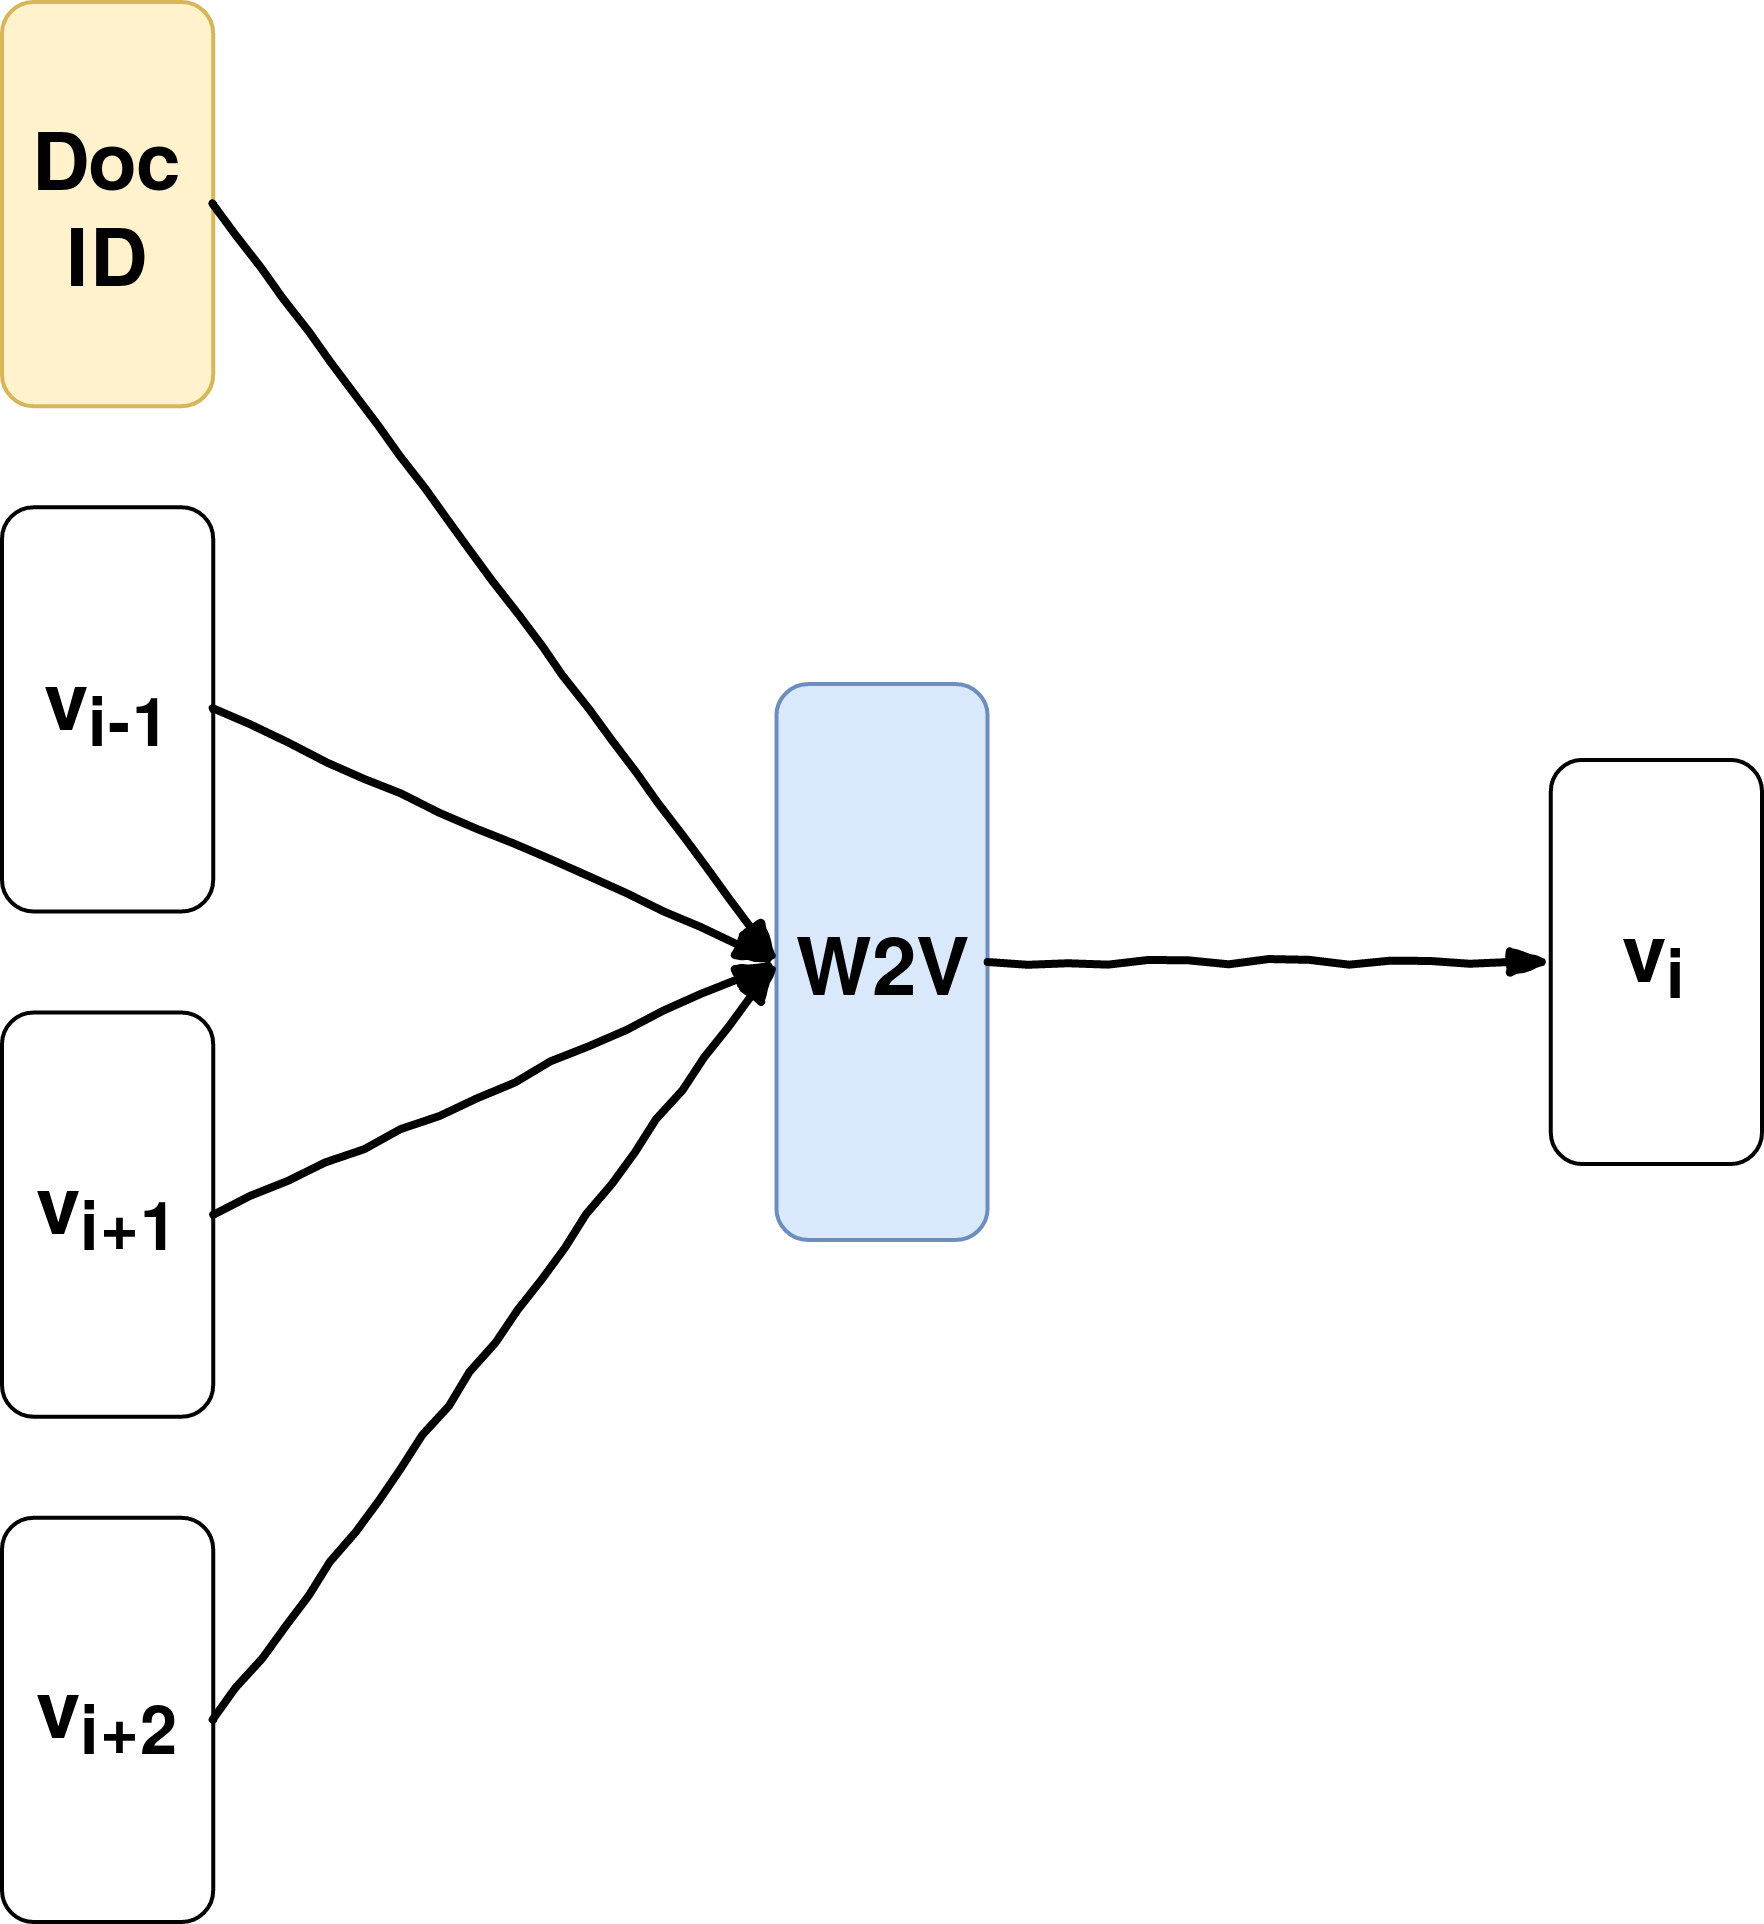
\includegraphics[width=0.5\textwidth,height=150px]{Doc2Vec}
	\caption{Doc2Vec PV-DM architektúra}
\end{figure}

A Word2Vec-hez hasonlóan a Doc2Vec-nek is létezik \textit{Skip-Gram} alternatívája, ez a PV-DBOW. A PV-DBOW modell gyorsabb és memóriahasználat szempontjából is gazdaságosabb a PV-DM-hez képest.

Mivel relatíve kevés algoritmus képes dokumentumszintű modellezésre és azok teljesítménye is limitált, a Doc2Vec egy jó választás lehet. A modell egyszerre mutat jó teljesítményt és a használata is könnyű.

\section{Transfer learning}

A modern szemantikus reprezentációs algoritmusok tanítása összetett folyamat. A feladatok során egyszerre kell több szempontra figyelni, melyek befolyásolhatják a modellünk pontosságát. Példának okáért mondatszintű reprezentációnknak képesnek kell lennie értelmezni a lexémák egymáshoz fűződő viszonyait és a mondatok közötti kohéziót is. A \textit{transfer learning} egy kiváló eszköz arra, hogy modellünket tanítsuk több aspektus szerint.

A \textit{transfer learning} napjainkban közkedvelt tanítási módszer, melynek ötletét az NLP ágazata a számítógépes látás eszközkészletéből merítette. A folyamatot két fázisra lehet bontani: előtanítás és a finomhangolás. Az előtanítás általában nagy mennyiségű adaton történik. A finomhangolás az előtanítás után kapott modell – adott NLP feladathoz szükséges – speciális feladatokon való tanítását jelenti, amely szignifikánsan kevesebb adatot igényel.

\begin{definition}
	Jelölje $D_s$ a forrástartományt, $D_t$ a céltartományt, $T_s$ a forrástartományhoz tartozó feladatot, továbbá $X_t$ és $Y_t$ rendre a $T_t$ célfeladathoz tartozó inputváltozók és  címkék halmazát. A \textbf{transfer learning} célja megtanulni $P(Y_t|X_t)$ feltételes eloszlást $D_t$-ben $D_s$ által gyűjtött információ alapján úgy, hogy $D_s \neq D_t$ vagy $T_s \neq T_t$.	 
\end{definition}

\begin{figure}[H]
	\centering
	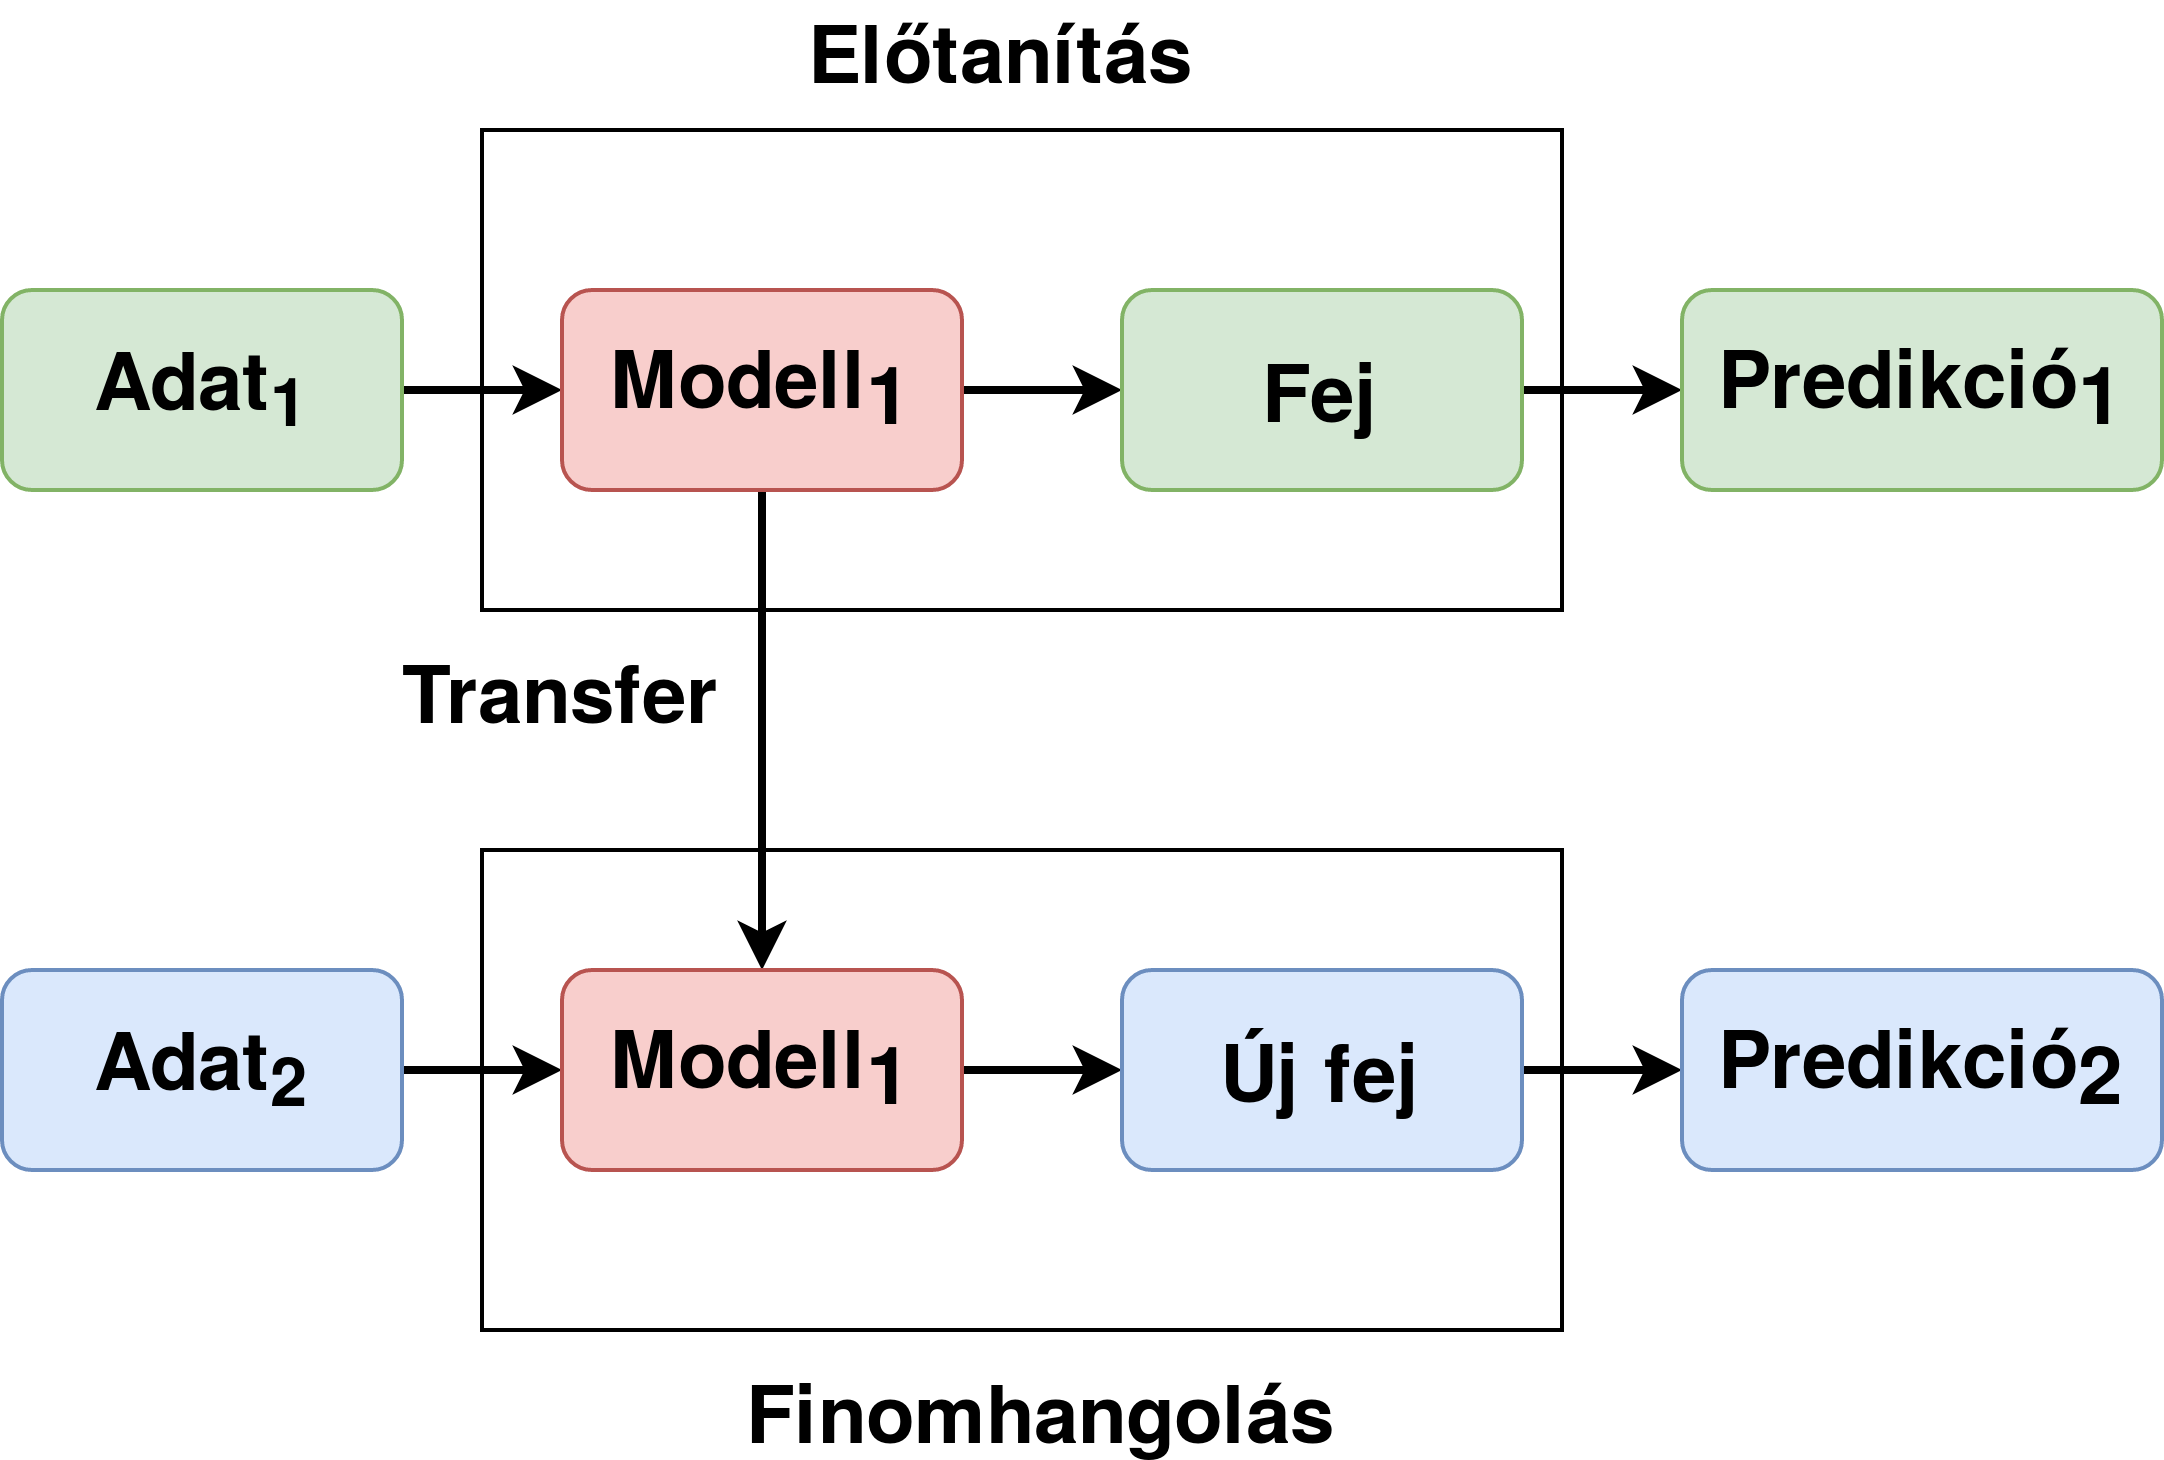
\includegraphics[width=0.6\textwidth,height=170px]{transfer}
	\caption{Transfer learning}
\end{figure}

Az előtanítási szakasz olyan feladattal kezdődik, mely kellőképpen generalizál és a neurális hálónk sok, hasznos és általános információhoz tud jutni. A folyamathoz használt adathalmaz általában nagy mennyiségű annotálatlan adatot tartalmaz, de vannak kivételek, például az InferSent esetében.

A finomhangolási fázis alatt használt feladatok az előtanítás után kapott modell súlyait alkalmazzák, de a bemeneti adatok és a feladatok végrehajtásához szükséges fej lehet eltérő is. Ezen szakasz állhat feladatok sorozatából is, ekkor a súlyokat inkrementálisan használják azok. A sikeres végrehajtást követően modellünk képes lesz komplexebb összefüggések felismerésére és pontosabb eredmény elérésére.

A jelenlegi trendek szerint a reprezentációs módszerek tanítási módja nagyobb hangsúlyt kap, mint maga a neurális háló szerkezete. A \textit{transfer learning} használata a numerikus ábrázolás során még kiaknázatlan terület, mely rendkívül sok eredményt hozhat a jövőben.








\cleardoublepage

\chapter{Az adathamazok és az előkészítés}
\label{ch:datasets}

Ahogy az előzmények fejezetben is láthattuk, a mai modern szemantikus reprezentációs modellek neurális hálók segítségével képezik le a nyelvi elemeket valamely vektortérbe. A neurális modellek a feladatok során felfedezik az adathalmaz rejtett mintáit és megtanulják az halmaz elemeinek eloszlását. Kevés adat esetén nem várhatjuk el a hálónktól a megfelelő pontosságot, mivel az adathalmazunk nem reprezentatív az adott problémára, továbbá a kis tanítóminta a túltanulás miatt is erősen eltérítheti a tanulási folyamatot.

Bár az olyan nyelveken, amelyeken a kutatásokat folytatják és amelyeket széles körben beszélnek előfordulhat ember által annotált adat is – ilyen például az SNLI – , a reprezentációs módszerek tanítását jellemzően auto-annotált adatokon végzik. Auto-annotált adatnak tekintünk minden olyan adatot, amelyek címkézését nem ember hajtotta végre. Az auto-annotált tanítóhalmazok hátulütője, hogy pontosságuk sokszor nem éri el az emberi szintet és jelentős zajt is tartalmazhatnak. A reprezentációs algoritmusok a kevesebb, de humán annotált halmazokon precízebb eredményt érnek el.

A magyar nyelv a kisebb körben használt nyelvek közé tartozik, így bátran vonhatjuk le azt a következtetést, hogy a web és egyéb források által hozzáférhető tartalmak mennyisége is erősen limitált. 
Munkám során fontos tényezőnek tartottam, hogy olyan jellegű adatokkal dolgozzak, melyek könnyen megszerezhetőek. Megfelelő választásnak bizonyultak a többnyelvű, publikus adathalmazok és az olyan profilú online elérhető dokumentumok, melyeket valamely webscraper-el össze lehet gyűjteni. Az így kialakult módszerek alkalmasak lehetnek arra, hogy akár más, kevésbé széleskörűen beszélt nyelvek esetén is alkalmazzák őket.

\subsection{Általános előkészítési lépések}

A nyers szöveg előkészítése elengedhetetlen folyamat az NLP feladatok során, mely nélkül értelmetlen eredményeket kapnánk. A jól elkülöníthető lépések után olyan kimenethez jutunk hozzá, amely lényegesen jobb feltételeket biztosít algoritmusunknak ahhoz, hogy képes legyen a dokumentumokat numerikusan értelmezni.

Az előkészítési szakasz a legtöbb esetben az úgynevezett token-ekre való bontással kezdődik. A \textbf{tokenizáció} a dokumentumok granularitásának növelésére szolgál. A bekezdéseket mondatokra, majd szavakra oszthatjuk, így hozzáférhetünk az olyan relációs információkhoz is, melyeket az alacsonyabb rétegek tárolnak.

Az adathalmaz \textbf{tisztítása}, vagy zaj csökkentése az olyan karakterek és karakterláncok eltávolítását jelenti, amelyek nem elemei a célnyelvnek. Adataink tartalmazhatnak akár speciális karaktereket, írásjeleket, HTML tag-eket, számokat és túl rövid – például 1 karakter hosszú – token-eket is, melyek megzavarhatják modellünk működését. A tisztítás során törölhetjük az adott nyelvben sűrűn előforduló szavakat (\textit{stopword}) is – például névelők – , így csak azok a token-ek maradnak a halmazban, amelyek valódi információtartalommal bírnak.

A szöveg \textbf{normálása} olyan módosításokat jelent, mely során az adathalmazunk token-eit azonos alakra hozzuk. A token-eket kis-, vagy nagybetűssé konvertálhatjuk, illetve a numerikus tartalommal rendelkező szavakat számokká alakíthatjuk. Természetesen ebben az esetben is célszerű törölni a numerikus token-eket, ha a tisztítás során is így jártunk el.

Megkülönböztethetünk két \textbf{szótövezési} formát, a \textit{stemming}-et és a \textit{lemmatization}-t. Mindkét módszernek az a célja, hogy eltávolítsa a ragokat a szótövekről. Míg a \textit{stemming} egy nyers heurisztikákon alapuló módszer, addig a \textit{lemmatization} pontosan próbálja meg szótári alakba konvertálni a szavakat szótár és morfológiai analízis segítségével. A normálás és szótövezés után egy csökkentett elemszámú szótárat kapunk, így az eredeti állapothoz közelítő pontossággal, de szignifikánsan kevesebb számítás- és memóriaigénnyel el tudja végezni az algoritmusunk a feladatát.

Az előkészítés végső lépése lehet az \textbf{n-gram}-ok bevezetése az adathalmazunkba. Az n-gram kifejezés egy n hosszú token szekvenciára utal, tehát a "New York" kifejezés 2-gram (bigram) lesz. Az n-gramok építése az n-gram modell feladata. A dokumentumhalmazunkon tanított n-gram modell az adott token prediktálását végzi el az előző $n-1$ token függvényében. Vegyük példának az előbbi bigram-ot:

\begin{equation}
\label{eq:n-grams}
P(\text{New York bigram}) = \frac{P(\text{A szám, ahányszor New és York egyszerre szerepelt})}{P(\text{A szám, ahányszor New szerepelt})}
\end{equation}

N-gram modellünk minden n hosszú token szekvencia esetén elvégzi a számítást, majd a legmagasabb előfordulási valószínűségű szópárokat "\_" jellel konkatenálja, tehát "New York" esetén New\_York-ot kapunk. Egy jól működő bigram modell elegendő lehet a feladatra, általában nincs szükség magasabb szintű összevonásra. A bigramok megkönnyíthetik nyelvi modellünk munkáját azzal, hogy a vélhetően összetett fogalmak különálló token-eit konkatenálják, így a tanítás során az algoritmusunk egy token-ként kezelheti a népszerű kifejezéseket.

Korábbi tapasztalataim azt mutatják, hogy a fenti technikák együttes alkalmazása lényegesen javíthatja az NLP feladatok megfelelő pontossággal való megoldásának esélyeit, ennél fogva a munkám során használt adathalmazok mindegyike maradéktalanul átesett az egyes előkészítési lépéseken.

A szótövezés során két \textit{lemmatizer} teljesítményét hasonlítottam össze, ezek a BSI beépített \textit{lemmatizer}-e és a HungarianSpacy. Az adathalmazok előkészítése alatt úgy tűnt, hogy a HungarianSpacy kevésbé mohó módszerrel vágja le a ragokat, ezért úgy döntöttem, hogy a továbbiakban azt használom, ugyanakkor nem vetem el annak a lehetőségét sem, hogy az erősebb szótövezés pontosabb végeredményt hozhat. 

Az implementációt Python nyelven végeztem, továbbá a Spacy és az NLTK nevű könyvtárakat használtam segítségül.

\subsection{Magyar wikipédia}
A Wikipédia a világ egyik legnagyobb többnyelvű, szabadon szerkesztett online enciklopédiája. Több, mint 6 000 000 dokumentumot tartalmaz, melyek egy-egy témakört, vagy fogalmat írnak le.

A szemantikus reprezentációs algoritmusok tanítása Wikipédia cikkeken nem új keletű ötlet. Számos nyelvi modell alapszik ezen az adathalmazon, többek között a BERT is.

Az online enciklopédia jól dokumentált alkalmazásprogramozási interfésszel rendelkezik, így tudtam én is hozzájutni a magyar nyelvű oldalak szövegéhez.

A letöltött nyers adathalmaz mérete összesen 2.4 GB, melynek a wiki-hu nevet adtam. A wiki-hu 459 286 darab magyar nyelven írt Wikipédia cikket, 16 301 289 sort és 150 333 446 token-t tartalmaz. 

A tanításhoz szükséges előkészítés után az adathalmaz mérete 2 GB-ra, a sorok száma 12 592 489-re a token-ek száma pedig 86 605 435-re csökkent.

A hozzáfűzött reményekkel ellentétben a magyar nyelvű cikkek relatíve elenyésző mennyiségben szerepelnek a Wikipédia adatbázisban. Következésképp a tanítóhalmaz nem bizonyult elegendőnek, így a továbbiakban csak a különböző technikák tesztelésére tudtam használni.


\subsection{OSCAR}

Az OSCAR (\textit{Open Super-large Crawled ALMAnaCH coRpus}) egy nyelvi klasszifikáló algoritmussal készült adathalmaz, melyet a szerzők a Common Crawl szétválogatásából és szűréséből kaptak, majd a sorait összekeverték. A Common Crawl egy 2011 óta gyűjtött publikus webarchívum. Az OSCAR magyar nyelvű szegmensének teljes mérete összesen 40 GB. 

Az előkészítési szakasz előtt szétválasztottam az adathalmazt két egyenlő részre, így két darab 20 GB-os szeletet kaptam. A továbbiakban az eredeti adatmennyiség első felével folytattam tovább az előkészületeket, melynek az oscar\_hu nevet adtam.

Az oscar\_hu nyers változata 127 654 271 darab sort és 5 168 152 283 darab token-t tartalmaz. Az előkészítési procedúra után 15 GB-ra csökkent a méret, 63 692 408 darab sor és 1 626 357 463 darab token maradt.

Ugyan az oscar\_hu nem tartotta meg a sorok közti relációkat, azonban az így kapott adatsokaság a mennyiségénél és annál a ténynél fogva, hogy a Word2Vec csak lokális információkkal dolgozik alkalmasnak bizonyult a szóbeágyazás tanítására.

\subsection{Hungarian Webcorpus}

A Hungarian Webcorpus a legnagyobb mai magyar nyelvű korpusz, melyet a Budapesti Műszaki Egyetem Média Oktató és Kutató Központja gyűjtött 2003-ban a SzóSzablya projekt keretein belül.

A korpusz 18 millió .hu domain-al rendelkező weboldal szövegéből áll, melyekből eltávolították a duplikált tartalmakat és az értelmetlen sorokat. Az így kapott dokumentumokra helyesírás ellenőrző szoftvert is futtattak. A publikált dokumentumok szavainak csupán 4\%-a volt felismerhetetlen a helyesírás ellenőrző szerint, így a végeredményben szereplő dokumentumok kevesebb nyelvtani hibát tartalmaznak, mint egy átlagos nyomtatott dokumentum. Az így kapott korpusz 589 millió szót tartalmaz, melyet 1221 millió magyar nyelvű weboldalról töltöttek le.

A letölthető fájlok ISO Latin-2 formátumban voltak, így az előkészítési folyamat előtt átkonvertáltam őket UTF-8 formátumba. Ez az átalakítás további megoldandó karakterproblémákhoz vezetett. A Hungarian Webcorpus mérete 18 GB volt, mely a tisztítási lépés után 7.8 GB-ra csökkent. A jelentős méretváltozás az XML tag-ek törlésére vezethető vissza. A token-izált változatban a méret tovább zsugorodott, így a végeredmény egy 6.6 GB-os adathalmaz lett.

A 1 221 405 darab fájl a tisztítás után összesen 127 711 725 darab sort és 589 209 017 darab token-t tartalmaz.

\subsection{Árukereső vélemények}
Az Árukereső a legnagyobb magyar online áruösszehasonlító oldal, melyen több mint 16 millió termék és 3 500 partner részletes adata szerepel. A felhasználóknak lehetőségük van anoním módon szövegesen véleményezni az adott kereskedőt, vagy árucikket, továbbá 1-től 5 csillagig osztályozni annak minőségét.

A weboldalon található adatokhoz egy saját kezűleg fejlesztett \textit{webscraper} segítségével jutottam hozzá. A halmaz mérete összesen 943 MB, amely 141 064 termék és 2209 áruház véleményeit tartalmazza. 

Az összesen 2 006 369 darab vélemény eloszlása a csillagok száma szerint a következő:

\begin{figure}[H]
	\centering
	\subfigure[Összes]{
		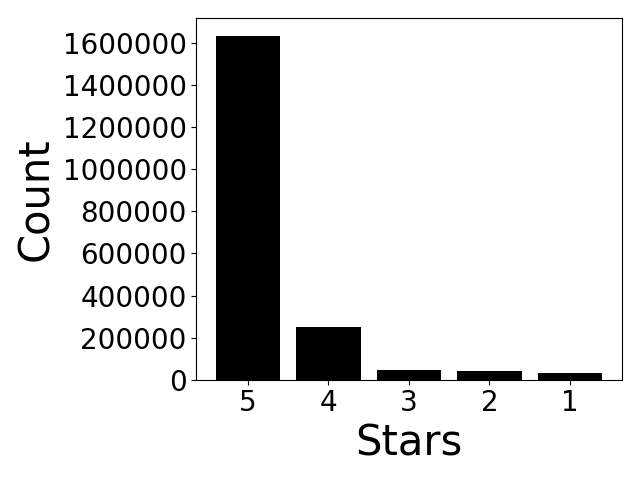
\includegraphics[width=0.45\linewidth]{arukereso}}
	\hspace{5pt}
	\subfigure[Legalább 10 hosszú]{
		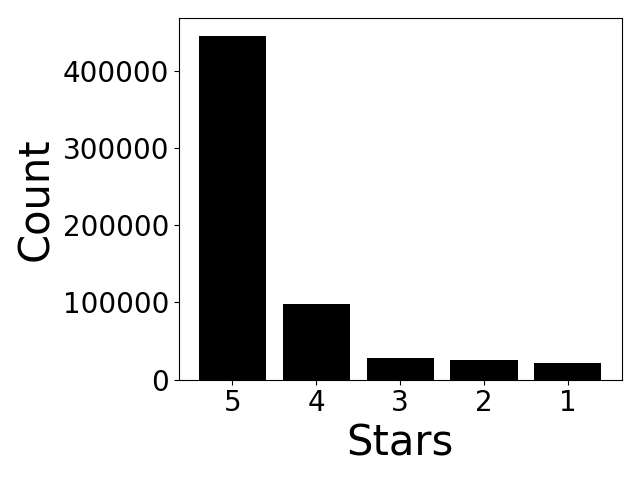
\includegraphics[width=0.45\linewidth]{arukereso10}}
	\caption{Vélemények eloszlása}
	\label{fig:example-2}
\end{figure}

A túl rövid vélemények kevés információval szolgálnak, így eltávolítottam az eredeti adathalmazból a 10 token-nál rövidebb véleményeket. A leghosszabb vélemény 842 token-ből áll.
\cleardoublepage

\chapter{A módszer leírása}
\label{ch:method}

A szemantikus reprenzentációs módszerek kutatása intenzíven felgyorsult az elmúlt évtizedben. Bár a szélesebb körben beszélt nyelvek esetében – például angol, kínai – számos technika és adathalmaz is elérhető, a kis és közepes nyelveknek egyelőre nélkülözniük kell ezeket. A probléma feltehetőleg részben a kutatási terület újszerű jellegéből, részben pedig a nagy tömegek igényeinek hiányából fakad. 

Ismereteim szerint magyar nyelven a tárgyalt kategóriák közül kizárólag szóbeágyazási modellek léteznek – mint a FastTex, Word2Vec és az ELMo – , továbbá a lehetséges tanítási feladatok is korlátozottak, így többnyire csak felügyelet nélküli tanítás elvégzése lehetséges. A diplomamunkám során megoldandó feladat egy mondat/paragrafus szintű nyelvi modell elkészítése, amely alapjául az előzményekben megismert módszerek szolgálnak. Továbbá olyan humán és autoannotált adathalmazok létrehozása, majd vizsgálata, melyeket a tanítási folyamathoz használok fel. Az így kapott előre tanított nyelvi modell reményeim szerint alkalmas lesz a későbbi NLP feladatokhoz szükséges finomhangolásra, továbbá a létrehozott adathalmazok és a tanításhoz használt algoritmusok más munkák segítségére is lehetnek.

A feladat megoldására szolgáló módszer alapvetően három részből áll: a bemeneti rétegből, a reprezentáció létrehozásához használt neurális hálóból és a modell tanításához definiált feladatokból, az ehhez alkalmazott fejekből. Mivel a szóalapú megoldások általában pontosabb eredményt mutatnak, mint a karakter, vagy szótöredék alapú modellek, így ebben az esetben is szavak kerülnek feldolgozásra.

\begin{figure}[H]
	\centering
	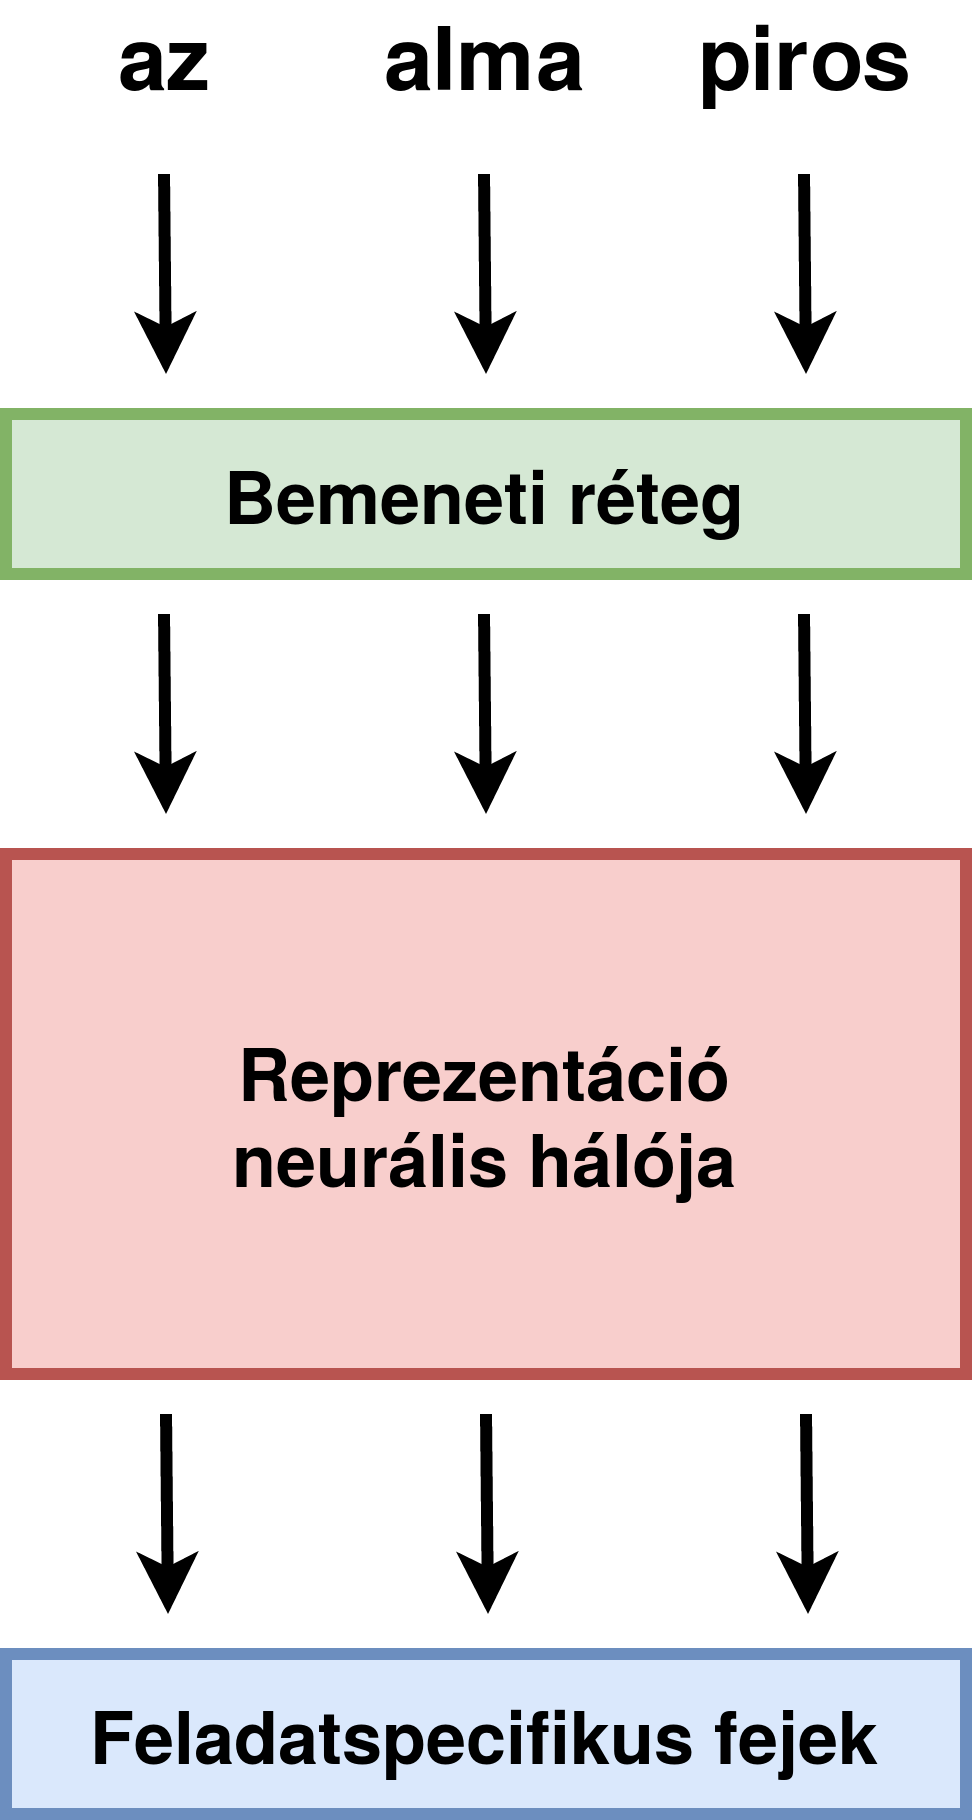
\includegraphics[width=0.3\textwidth,height=220px]{architecture}
	\caption{A módszer magasszintű architektúrája}
\end{figure}

Az implementációt Python nyelven végeztem a Tensorflow \cite{tensorflow} nevű könyvtár segítségével.

\section{Bemeneti réteg}

Ahogyan több módszer esetén is láthattuk, előfordulhat, hogy a neurális hálók bemenetére már eleve vektorizált formában érkeznek a token-ek. A feladat megoldásához használt architektúrában az input koordinálását egy bemeneti réteg végzi. Ezen réteg a felhasználó által konfigurálható attól függően, hogy az inputra a token-ek enkódolt formában érkeznek, vagy az algoritmus a számára megadható szóbeágyazási modellt használja. Ha a token-ek nem vektor formájában kerülnek a bemenetre, akkor a bemeneti réteg a token-ekhez rendelt egyedi azonosító számok szekvenciáját fogadja.

A tanítás során minden esetben a mélyháló számára megadott Word2Vec - CBOW szóbeágyazási modelleket használtam, melyek 300 dimenziós szóvektorokat tartalmaznak. A szóbeágyazások tanítóalgoritmusa 5 token széles ablakot alkalmazott. Az előtanítás során átadott reprezentációs mátrixot a GPU a memóriában tárolja és műveleteket is végez vele, ezért a nagyobb, oscar\_hu halmazon tanított modell rendkívül memóriaigényesnek, továbbá a wiki\_hu tanítóhalmaz – a Word2Vec tanításához – túl kisméretűnek bizonyult. Így a végső választás az oscar\_sm modellre esett, ami az oscar modell kisebb méretű szótárral rendelkező változata. A wiki\_hu 658 129, az oscar modell 2 335 673, az oscar\_sm pedig 645 136 darab vektorból áll.

\begin{figure}[H]
	\centering
	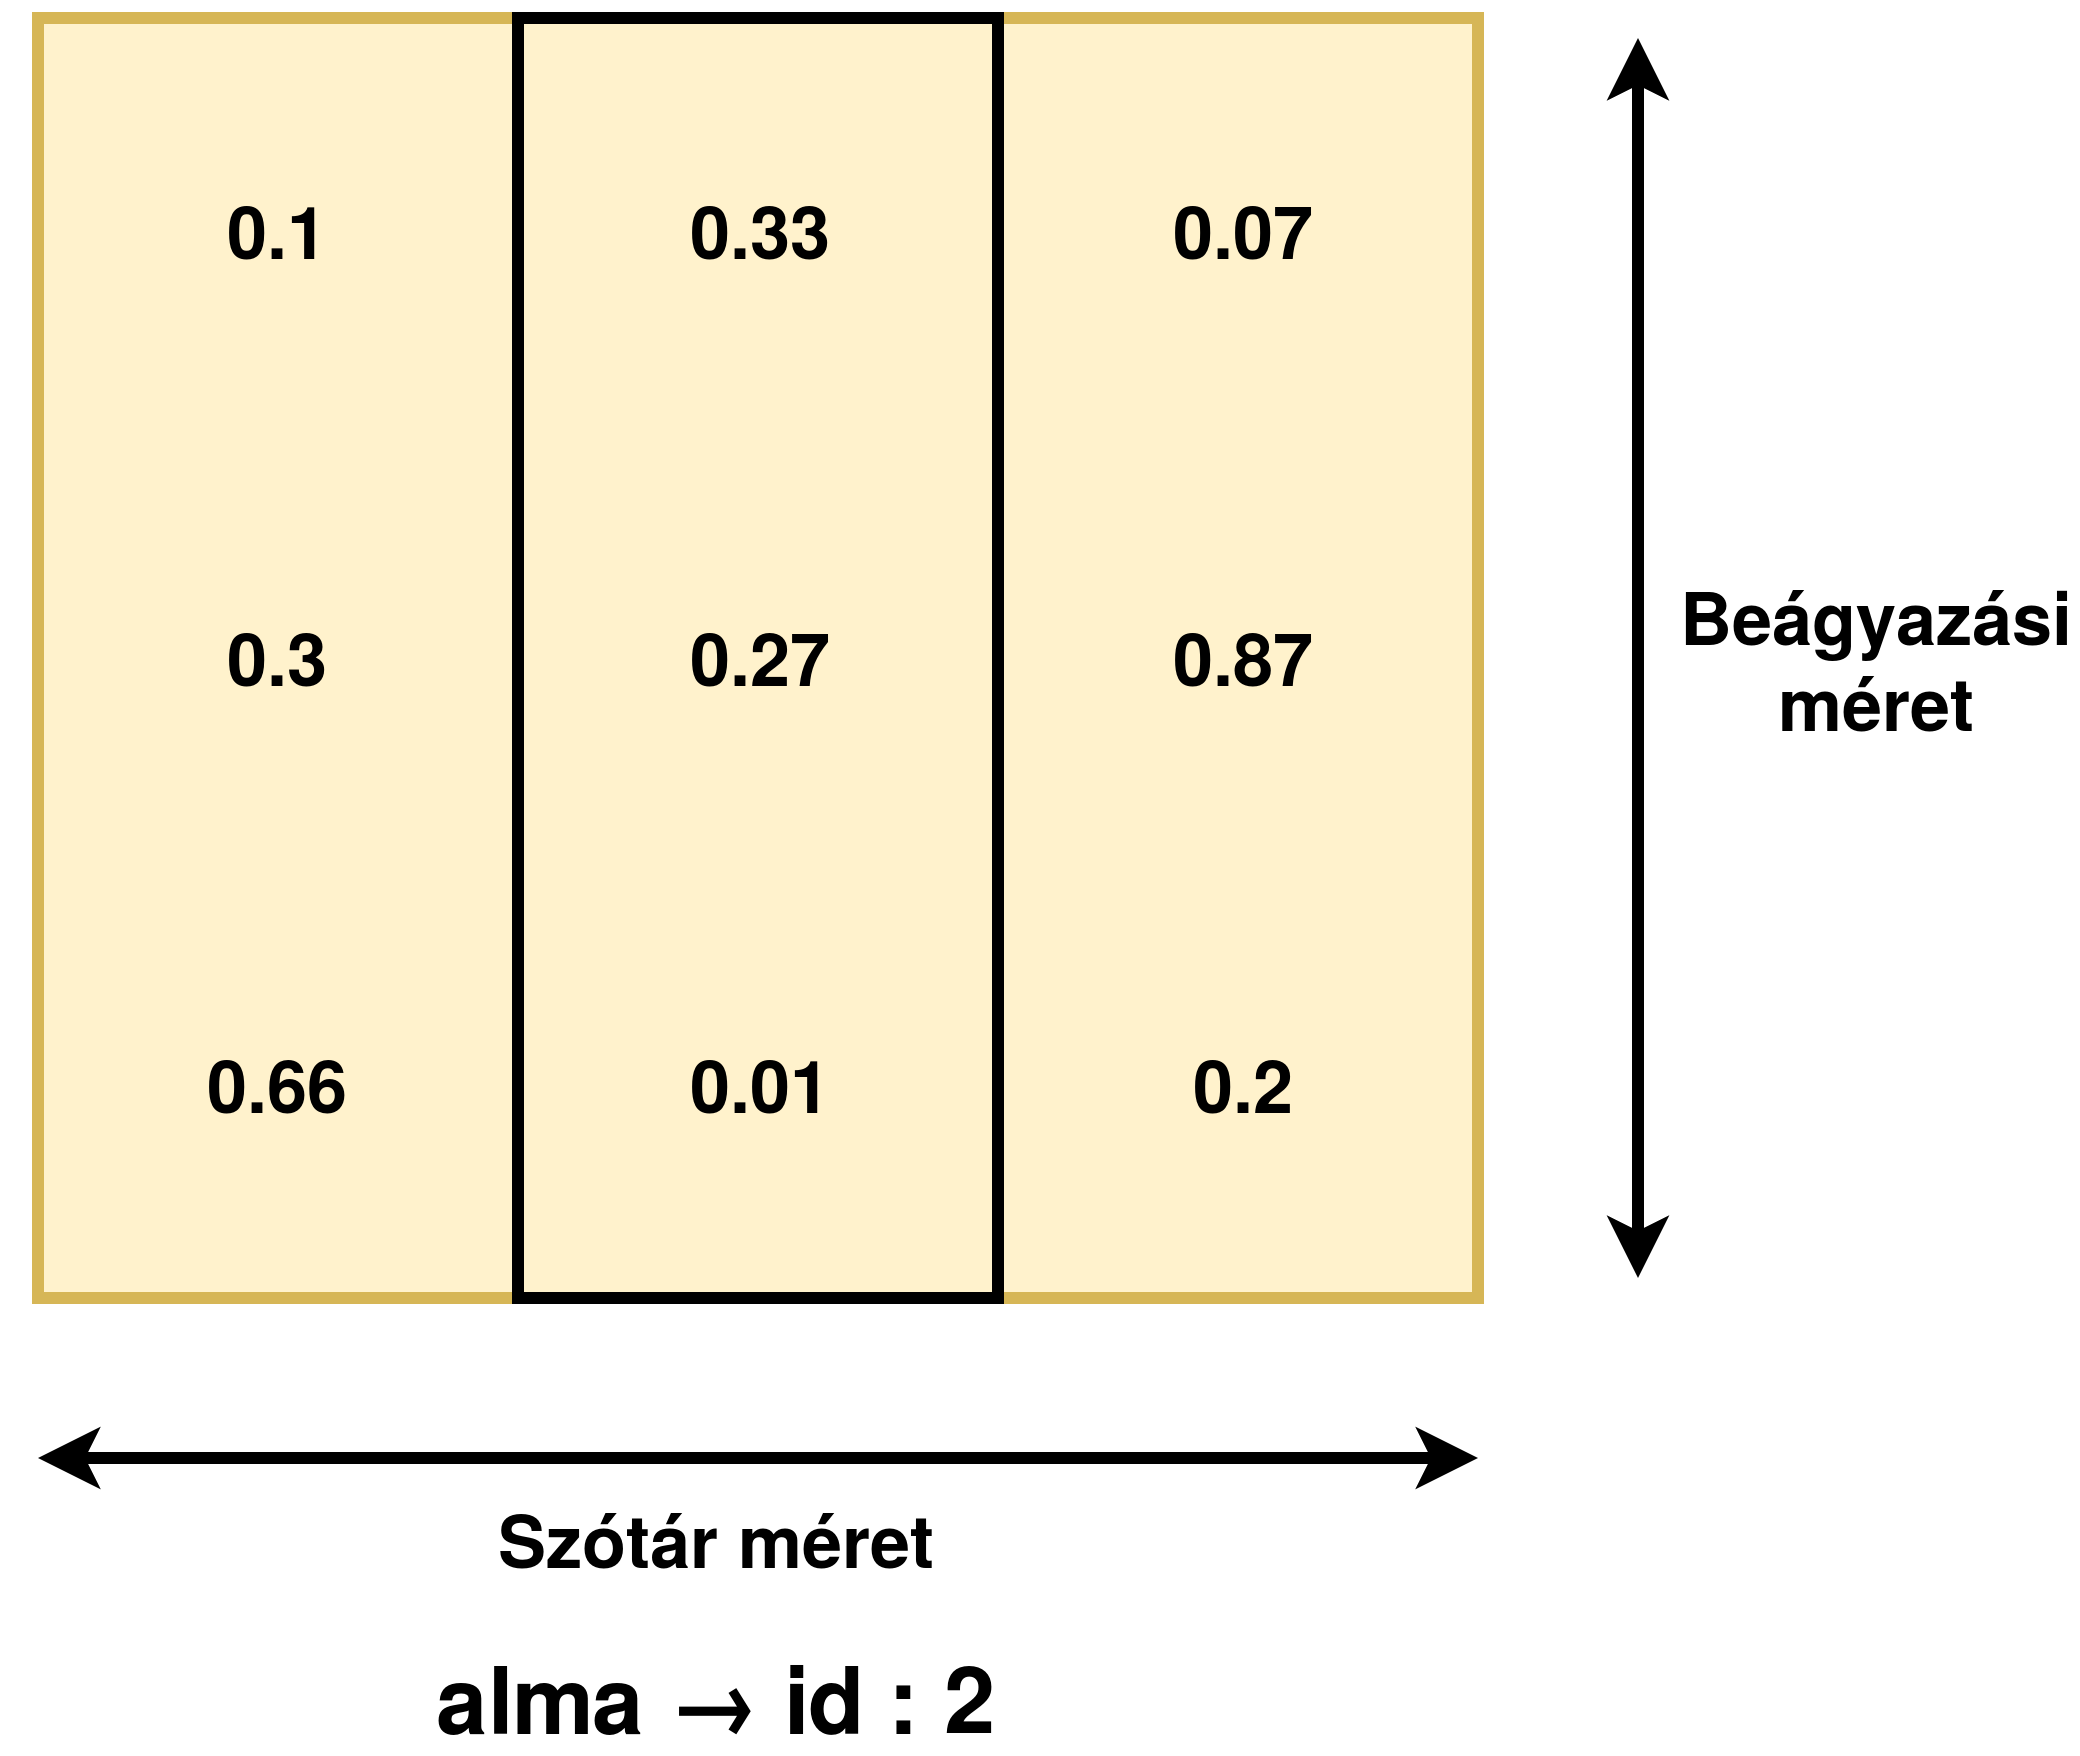
\includegraphics[width=0.6\textwidth,height=220px]{embedding}
	\caption{Az embedding lookup}
\end{figure}

A bemeneti réteg fix súlyokkal rendelkezik, tehát a tanulási folyamat során nem változtatja azokat. A mélyháló a számára átadott beágyazási mátrix elemei közül kikeresi az azonosítóknak megfelelő elemeket, majd továbbítja őket a kimenetre. Ezt a folyamatot \textit{embedding lookup}-nak nevezzük.

\section{A reprezentáció neurális hálója}

A rekurrens neurális hálók (RNN) használata a szemantikus reprezentációs modellek esetén gyakori technika. Míg a mesterséges neurális hálók (ANN) csak önálló bemenet fogadására képesek, addig a rekurrens neurális hálók alkalmasak szekvenciális input feldolgozására is. Ilyen szekvencia például az idősori, vagy a szöveges adat is. A szekvenciális bemenetet az a tulajdonság különbözteti meg önálló bemenettől, hogy az input elemei függenek egymástól, hatással lehetnek a szomszédaikra, több önálló input esetén ez a reláció nem érvényes.

A rekurrens neurális hálók képesek megtanulni az adatsor elemei közötti kapcsolatokat. Az RNN a tanulási folyamat során "emlékszik" az előző elemektől gyűjtött információkra, majd azok segítségével generálja a kimenetet/kimeneteket. A számítás során használt vektorokat nem csak az input súlyai befolyásolják, hanem a rekurrens háló rejtett állapotvektorai is. A rejtett állapot megtanulja a folytonos bemenet elemei közti függőségeket, majd minden tanítási lépés során frissül. Ennélfogva minden egyes bemeneti elem más és más műveleten esik át.

\begin{figure}[H]
	\centering
	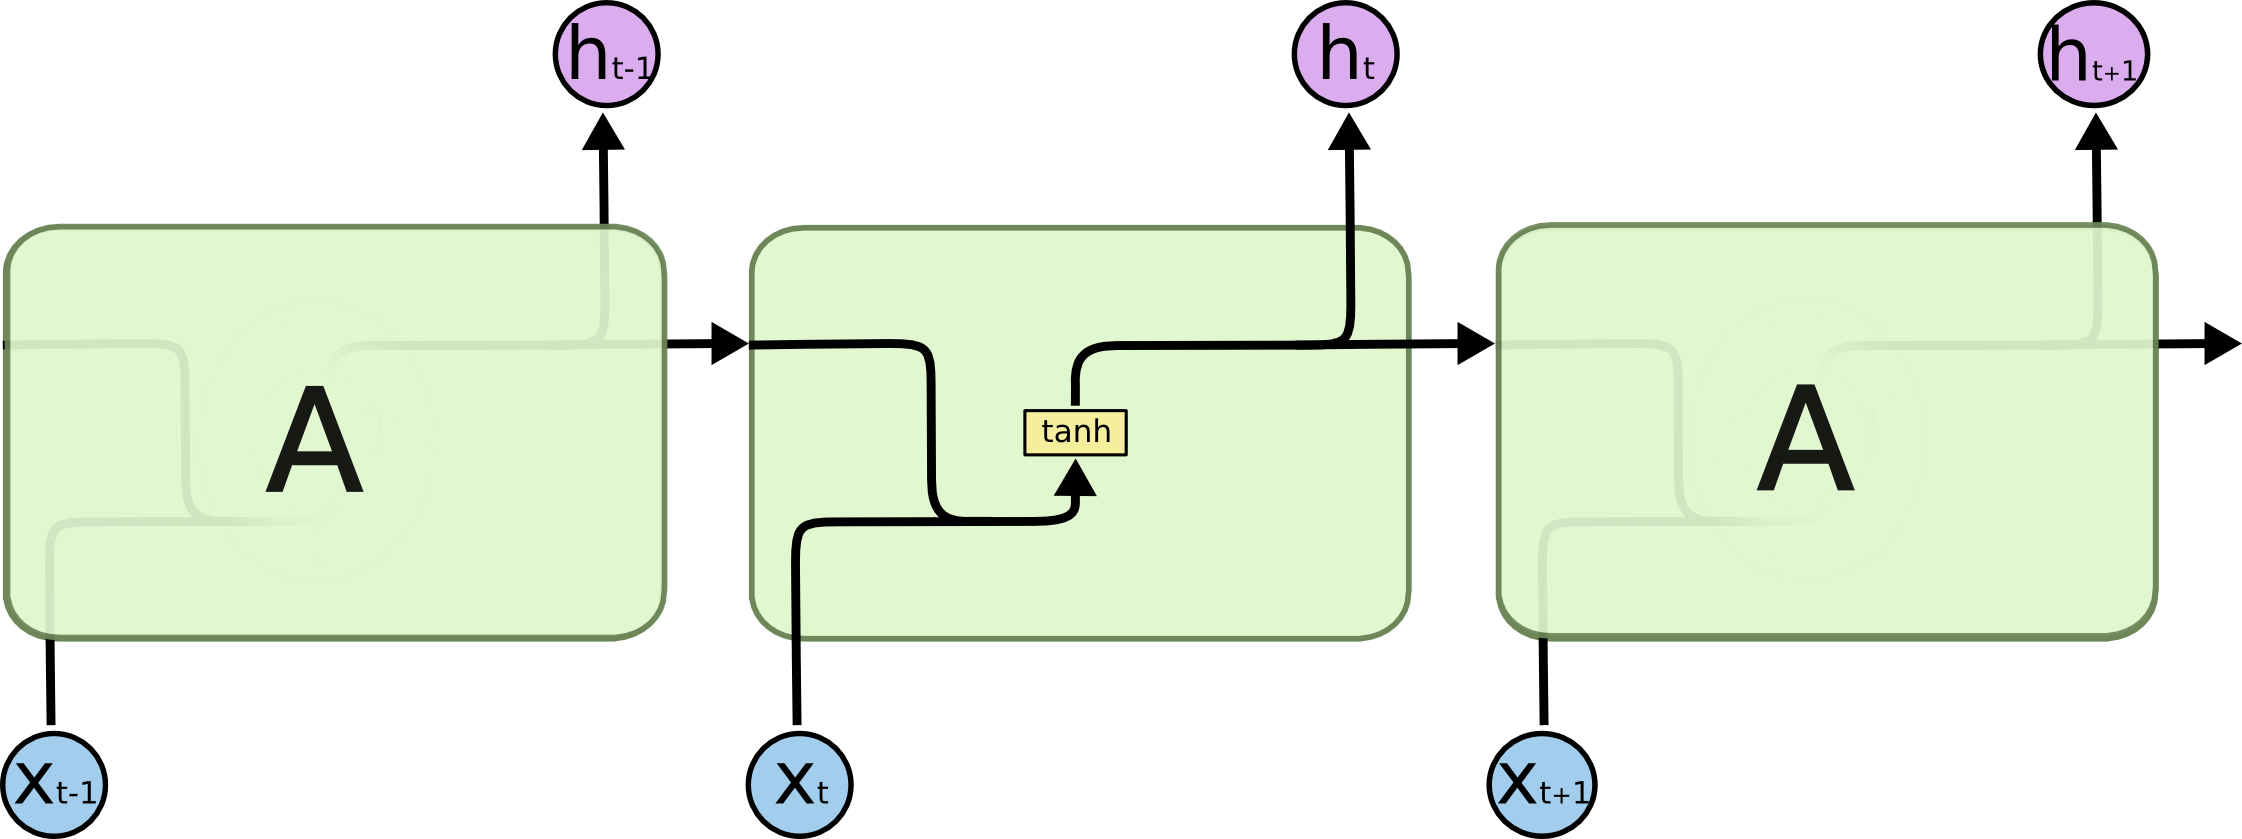
\includegraphics[width=0.55\textwidth,height=100px]{rnn}
	\caption{Az RNN cella \cite{rnn}}
\end{figure}

Bizonyos esetekben, ahol a múltból származó információ elegendő lehet a háló számára – például következő token generálása az előzőek függvényében – , az egyszerű RNN jó opció lehet. Azonban olyan feladatok során, melyeknél fontos a bemeneti adatok kontextusa – például a nyelvi modellek – , más megoldásra van szükség. A BiRNN architektúra lényege, hogy az inputot két, egymással ellentétes irányú rekurrens háló olvassa. Az így kapott kimeneti vektorok páronkénti konkatenációja lesz a BiRNN output-ja.

\begin{figure}[H]
	\centering
	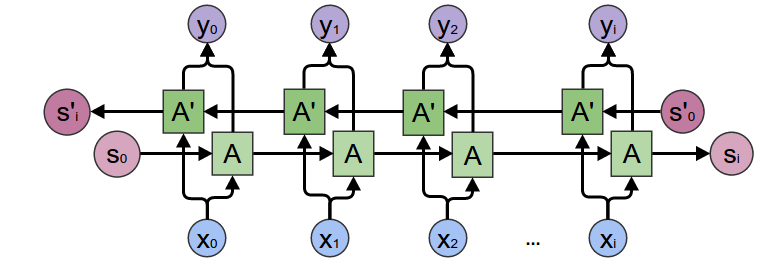
\includegraphics[width=0.7\textwidth,height=120px]{birnn}
	\caption{A BiRNN architektúra \cite{birnn}}
\end{figure}

Az RNN-ek legegyszerűbb formájának (\textit{Vanilla RNN}) azonban van egy nagy gyengesége, ami a hosszútávú információkat illeti. Gradiensnek hívjuk azokat az értékeket, melyeket a háló a súlyai frissítésére használ. Vanilla RNN esetén a visszaterjesztési művelet (\textit{backpropagation}) alatt annyira lecsökkenhetnek az eleve túl kicsi gradiensek, hogy a hozzá tartozó rétegek megállnak a tanulásban. Ezt a problémát a \textit{vanishing gradients} problémának hívjuk.

Az LSTM (\textit{Long short-term memory}) architektúra megoldást nyújt a \textit{vanishing gradient} problémára. Az LSTM a megszokott hosszútávú memória mellé bevezeti a rövidtávú memóriát is. Olyan belső műveletei vannak, melyek képesek szabályozni az adott cellán belüli információáramlást. Ezen műveleteket kapuknak nevezzük. A kapuk eldönthetik, hogy mely információ lesz fontos a továbbiakban és melyiket lehet törölni. Így a módszer csak releváns információt enged a hosszútávú memóriába.

\begin{figure}[H]
	\centering
	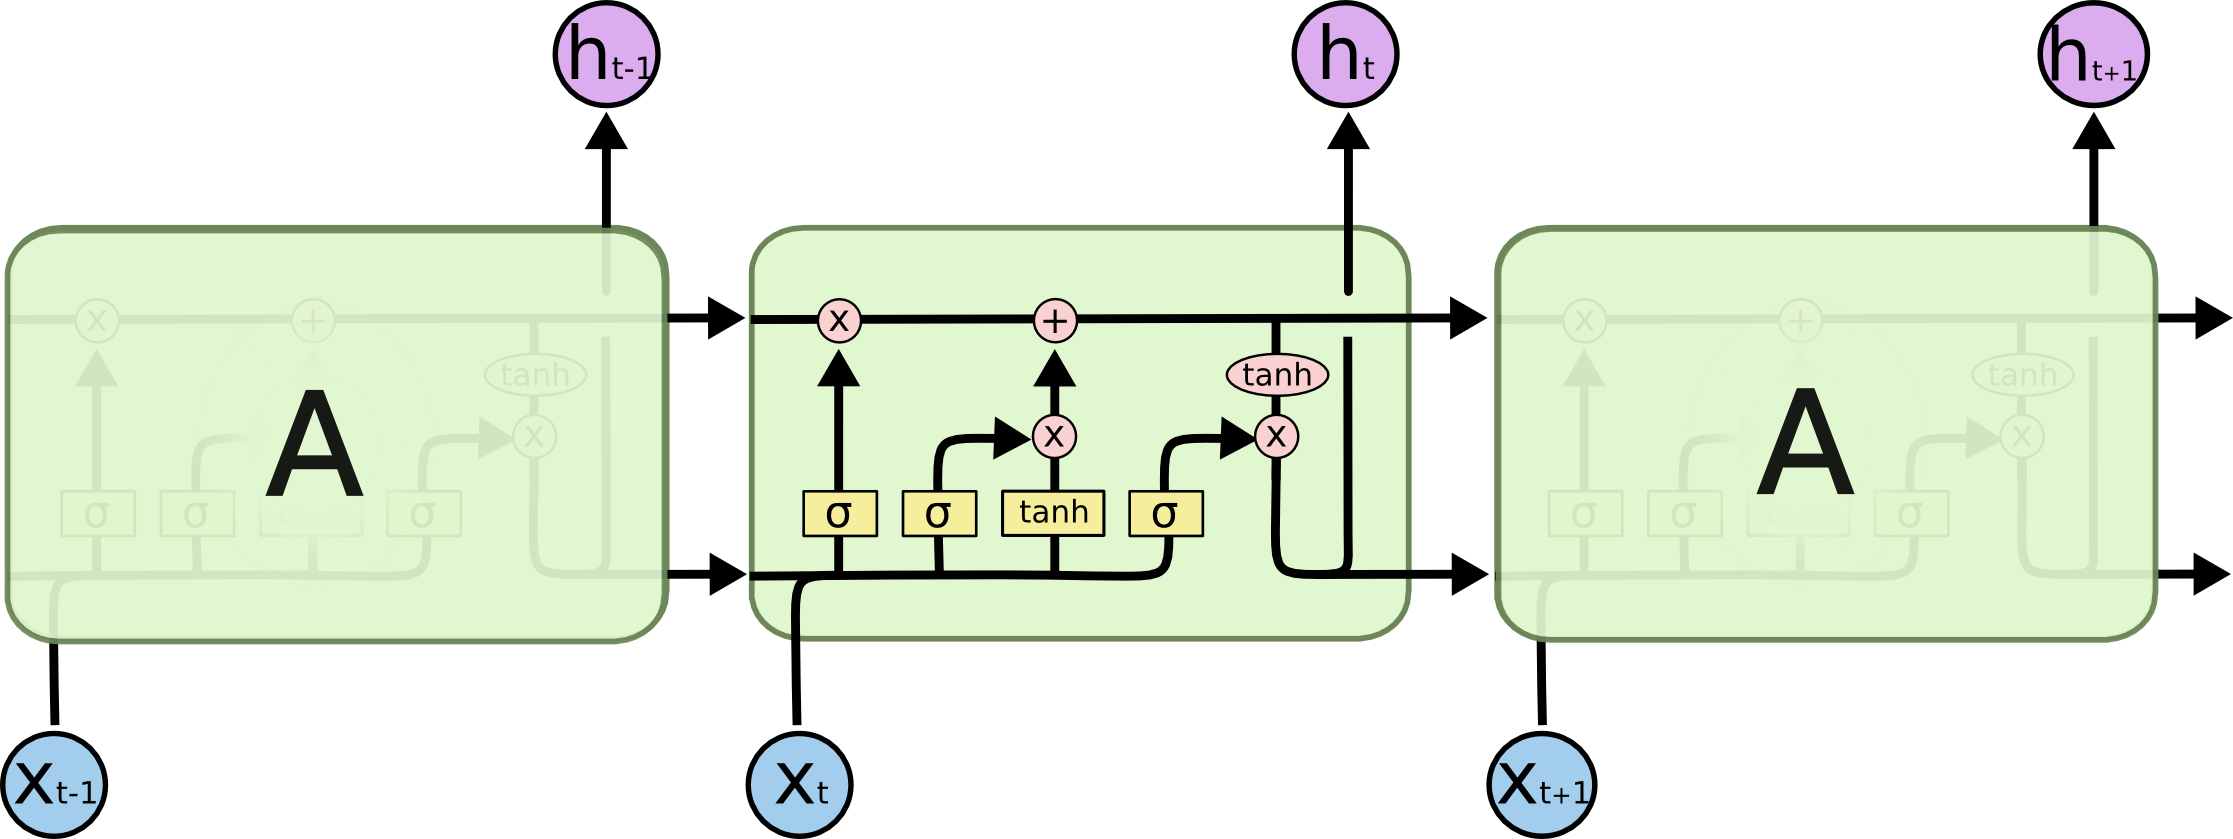
\includegraphics[width=0.55\textwidth,height=100px]{lstm}
	\caption{Az LSTM cella \cite{rnn}}
\end{figure}

Az általam a feladat megoldására választott architektúra az InferSent-ben kiváló eredményeket prezentáló BiLSTM + Max Pooling.

\subsection{A BiLSTM}
A BiLSTM egy kétirányú rekurrens neurális háló (BiRNN), amely LSTM cellákat használ. Az NLP feladatok természetes nyelven írott szöveggel operálnak, így a rekurrens neurális háló az egyik alternatíva a változó hosszúságú szekvenciális adat feldolgozására. A kétirányú modell figyelembe veszi a feldolgozandó token kontextusát a tanulás során és eltárolja a sorrendi információkat is. Az LSTM cellák alkalmazása széles körben elterjedt technika, amely amellett, hogy képes kezelni az RNN gyengeségeit, a jelenlegi egyik legpontosabb megoldásnak bizonyul.

\begin{figure}[H]
	\centering
	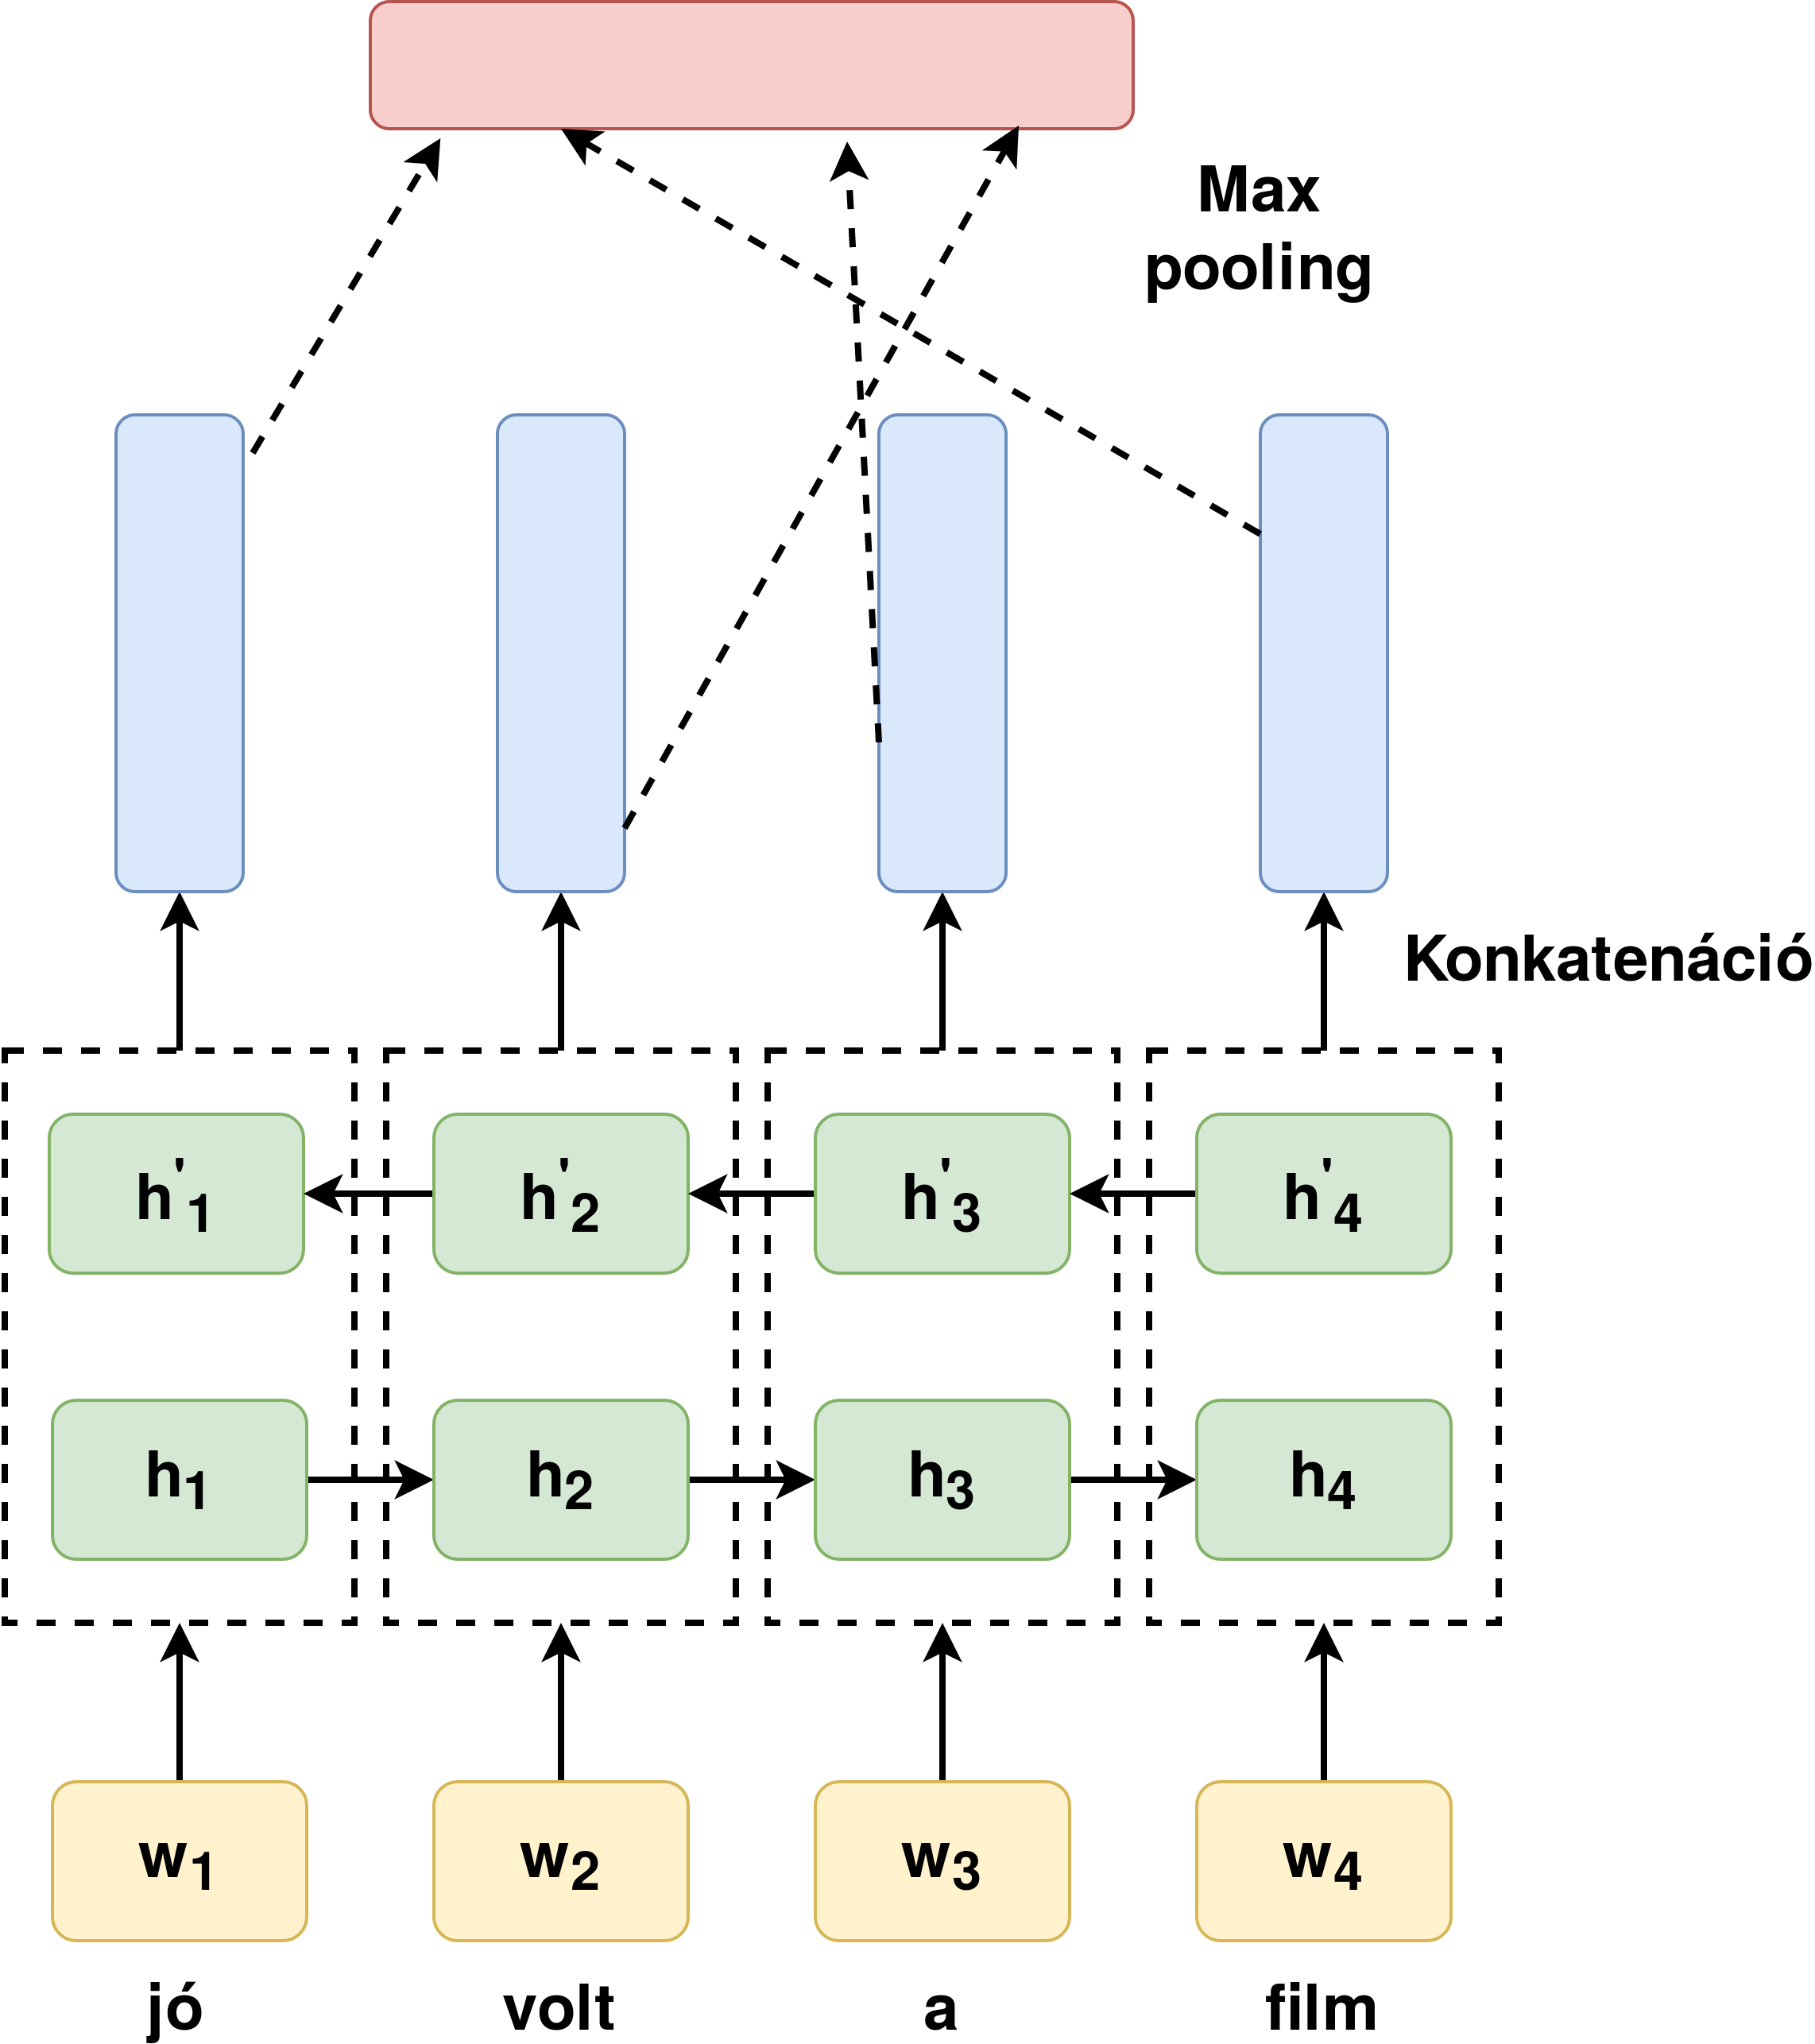
\includegraphics[width=0.45\textwidth,height=180px]{biLSTM-max-pooling}
	\caption{A BiLSTM + max pooling architektúra}
\end{figure}

A sűrű rétegek tanítása közben az egyes neuronok között kialakulhatnak keresztfüggőségek, így túltanulhat a modellünk az adott adathalmazra. A \textit{dropout} egy olyan regularizációs technika, amely kikényszeríti, hogy az egyes neuronok önállóan tanuljanak, így véd a túltanulás ellen és a neurális háló is jobban fog generalizálni. A tanítási fázis során az összes iteráció, összes batch-e esetén minden neuron és hozzá tartozó aktiváció $1-p$ valószínűséggel véletlenszerűen kidobásra kerül. A teszt fázis alatt az összes neuron cselekvőképes, de az aktivációkat a helyes működés miatt $p$ állandóval szorozni kell. Bár a tanítási idő minden \textit{epoch} során kevesebb lesz, a \textit{dropout} körülbelül duplázza a konvergációhoz szükséges iterációk számát. A reprezentáció tanulására szolgáló neurális háló mindkét LSTM rétegére konfigurálható \textit{dropout}-ot alkalmaztam.

\begin{figure}[H]
	\centering
	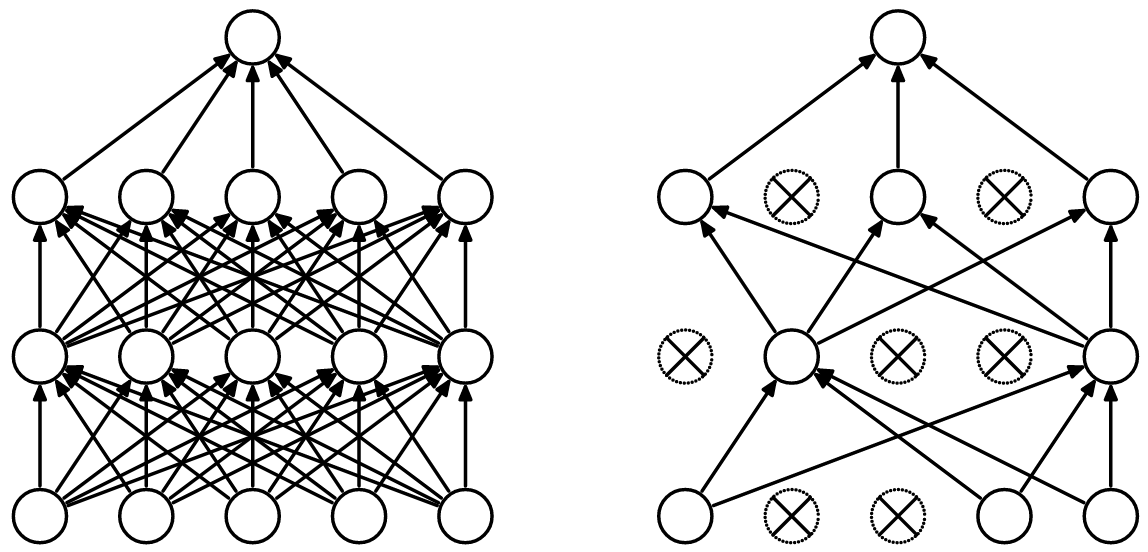
\includegraphics[width=0.6\textwidth,height=140px]{dropout}
	\caption{A dropout vizualizációja \cite{dropout}}
\end{figure}

A BiLSTM réteg által generált szekvenciális kimenet egy \textit{pooling} rétegbe vezet.

\subsection{Pooling réteg}

A \textit{pooling} ötletét szintén a számítógépes képfeldolgozás ágazatától kölcsönözte az NLP. Míg a konvolúciós rétegek esetén a \textit{feature map}-ek kisebb szegmensein elvégzendő a \textit{pooling} művelet, addig az NLP-ben vektorokra értendő.
A \textit{max pooling} réteg a kapott bemenet megadott tengelyei mentén választja ki a legnagyobb értékeket. Analóg módon a \textit{mean pooling} az átlagot veszi alapul.

A BiLSTM-ben található rejtett rétegek kimeneteinek páronkénti konkatenációján végzett pooling művelet képes kiválasztani a hasznos információkat az egyes token-eket/részszekvenciákat reprezentáló vektorokból. Az így kapott sorvektor lesz a szöveges bemenet végső reprezentációja.

A nyelvi modell neurális hálójának implementációja egy konfigurálható \textit{pooling} réteget tartalmaz, így a megoldás \textit{max} és \textit{mean pooling}-gal, továbbá pooling nélkül is képes dolgozni.

\subsection{Paraméterek és konfigurálhatóság}

A módszer neurális hálójának implementációja során törekedtem a minél széleskörűbb konfigurálhatóságra, így elősegítve a könnyebb testreszabhatóságot és az újrafelhasználhatóságot. 

A felhasználó által állítható, modellre vonatkozó paraméterek a következők:
\begin{itemize}
	\item \textit{use\_embedding\_layer} : Alkalmazzon a háló bemeneti réteget, vagy vektorizált az input.
	\item \textit{word\_embedding\_dim} : A bemeneti szóbeágyazási vektorok mérete.
	\item \textit{num\_hidden} : A végső reprezentáció mérete, a rejtett LSTM rétegek méretének kétszerese.
	\item \textit{dropout\_keep\_prob} : Dropout valószínűség.
	\item \textit{pooling} : \textit{Pooling} fajtája. (Max, Mean)	
\end{itemize}

A neurális háló paraméterezhetősége lehetőséget biztosít arra, hogy az architektúra más típusú bemenettel, más célra is felhasználható legyen. Ezen konfigurációkon felül több, a tanítási folyamathoz kapcsolódó érték is állítható.

\section{Tanítás}

Bár az alkalmazott architektúra teljesítménye jelentősen hozzájárul a szemantikus reprezentációs modellek pontosságához, az elmúlt néhány év során mégis inkább a tanítóhalmazok és a tanítási módszerek felé irányult a figyelem.

A neurális hálóknak a korábbi hagyományos, feladatspecifikus tanítás alatt egyszerre kellett megérteni a dokumentumhalmaz nyelvét és megtanulni az adott feladathoz szükséges ismereteket. A \textit{transfer learning} technika segítségével ez a két folyamat különválasztható. Az előtanulás során feldolgozott nagy mennyiségű adat hatására a háló megragadja a dokumentumok nyelvi sajátosságait, így a finomhangolás alatt a modell koncentrálhat csak az adott feladatra. Az eredmény legtöbbször egy jobban működő reprezentáció.

Az előtanítási feladatok olyan jellegű kihívások elé állítják a reprezentáció neurális hálóját, amelyek során egy erős, általános tudást képes megszerezni. A probléma megoldására implementált feladat a BERT előtanításához hasonló \textit{multi-task learning}. 

A \textit{multi-task learning} egyszerre több feladaton történő tanulást jelent, ami jobb generalizációra készteti a hálót. Az egyik feladat a \textbf{maszkolás}, amely az egyes szavak közötti szemantikai és szintaktikai relációk ábrázolását támogatja. A másik feladat a \textbf{következő mondat}, mely a mondatok közötti kohézió reprezentációját segíti.

Mivel az említett feladatok számára tanítóadatot bármely célnyelvű korpuszból könnyedén lehet generálni, ezért elméletileg az előtanítás a végtelenségig skálázható. Az input előállítása során a \textit{hungarianWebcorpus} nevű adathalmazzal dolgoztam, mivel az jelentős mennyiségű szöveges adatból áll, és a mondatok az \textit{oscar\_hu} adathalmazzal ellentétben sorrendtartóak.

A generálás során az algoritmus rögzített token-számú szekvenciákra osztotta a korpuszt. Olyan esetben, mikor nem volt elég token a szekvencia kitöltésére – például rövid dokumentumok, dokumentumvégek – , "[PAD]" speciális helykitöltő \textit{padding} token-eket konkatenált a dokumentum szavaihoz. 
 
A maszkolás a BERT-ben alkalmazott technika alapján történt: az algoritmus az előállított token-szekvenciák elemeinek 15\%-át véletlenszerűen kiválasztotta. 
\begin{itemize}
	\item A kiválasztott token-ek 80\%-át a "[MASK]" speciális token-nel helyettesítette. 
	\item 10\%-át a szótárból választott véletlenszerű szóra cserélte.
	\item A maradék 10\% esetében maradt az eredeti token.
\end{itemize}

A BERT szerzője szerint, ha a maszkolt token-ek 100\%-át prediktálná a rendszer, akkor nem feltétlen lenne képes megfelelő minőségű reprezentációt generálni a nem maszkolt szavaknak. Ha a kiválasztott token-ek 90\%-át maszkolná és 10\%-ot random választott szóval helyettesítene, az arra késztetné a modellt, hogy úgy gondolja, az adott szó soha nem helyes. Ha pedig a kiválasztott token-ek 90\%-át maszkolná és 10\% maradna az eredeti szó, a modell lemásolná a nem kontextusfüggő beágyazásokat. \cite{bertappendix}

A \textit{következő mondat} feladathoz szükséges "mondatpárokat" az így előállított tokenszekvenciákon végigiterálva generálta az algoritmus. $S$ szekvenciát $0.5$ valószínűséggel $S$ után következő szekvenciával, $0.5$ valószínűséggel a korpuszból választott véletlenszerű szekvenciával konkatenálta. A két szekvencia közé egy speciális "[SEP]" mondathatárt jelző token-t illesztett. A végső adathalmaz az így kapott A[SEP]B alakú maszkolt, fix méretű szekvenciákból álló halmaz, mely mérete $13.3$ GB.

\begin{note}
A "mondat" szó ebben az esetben token-ek tetszőleges méretű sorozatát jelenti.
\end{note}
 
A bemenet előállításához szükség volt arra az információra, hogy maximum hány token hosszúságú szekvenciákra darabolja az algoritmus a dokumentumokat és mi a minimális soronkénti token-szám, amelyet még elfogadjon. 

\begin{figure}[H]
	\centering
	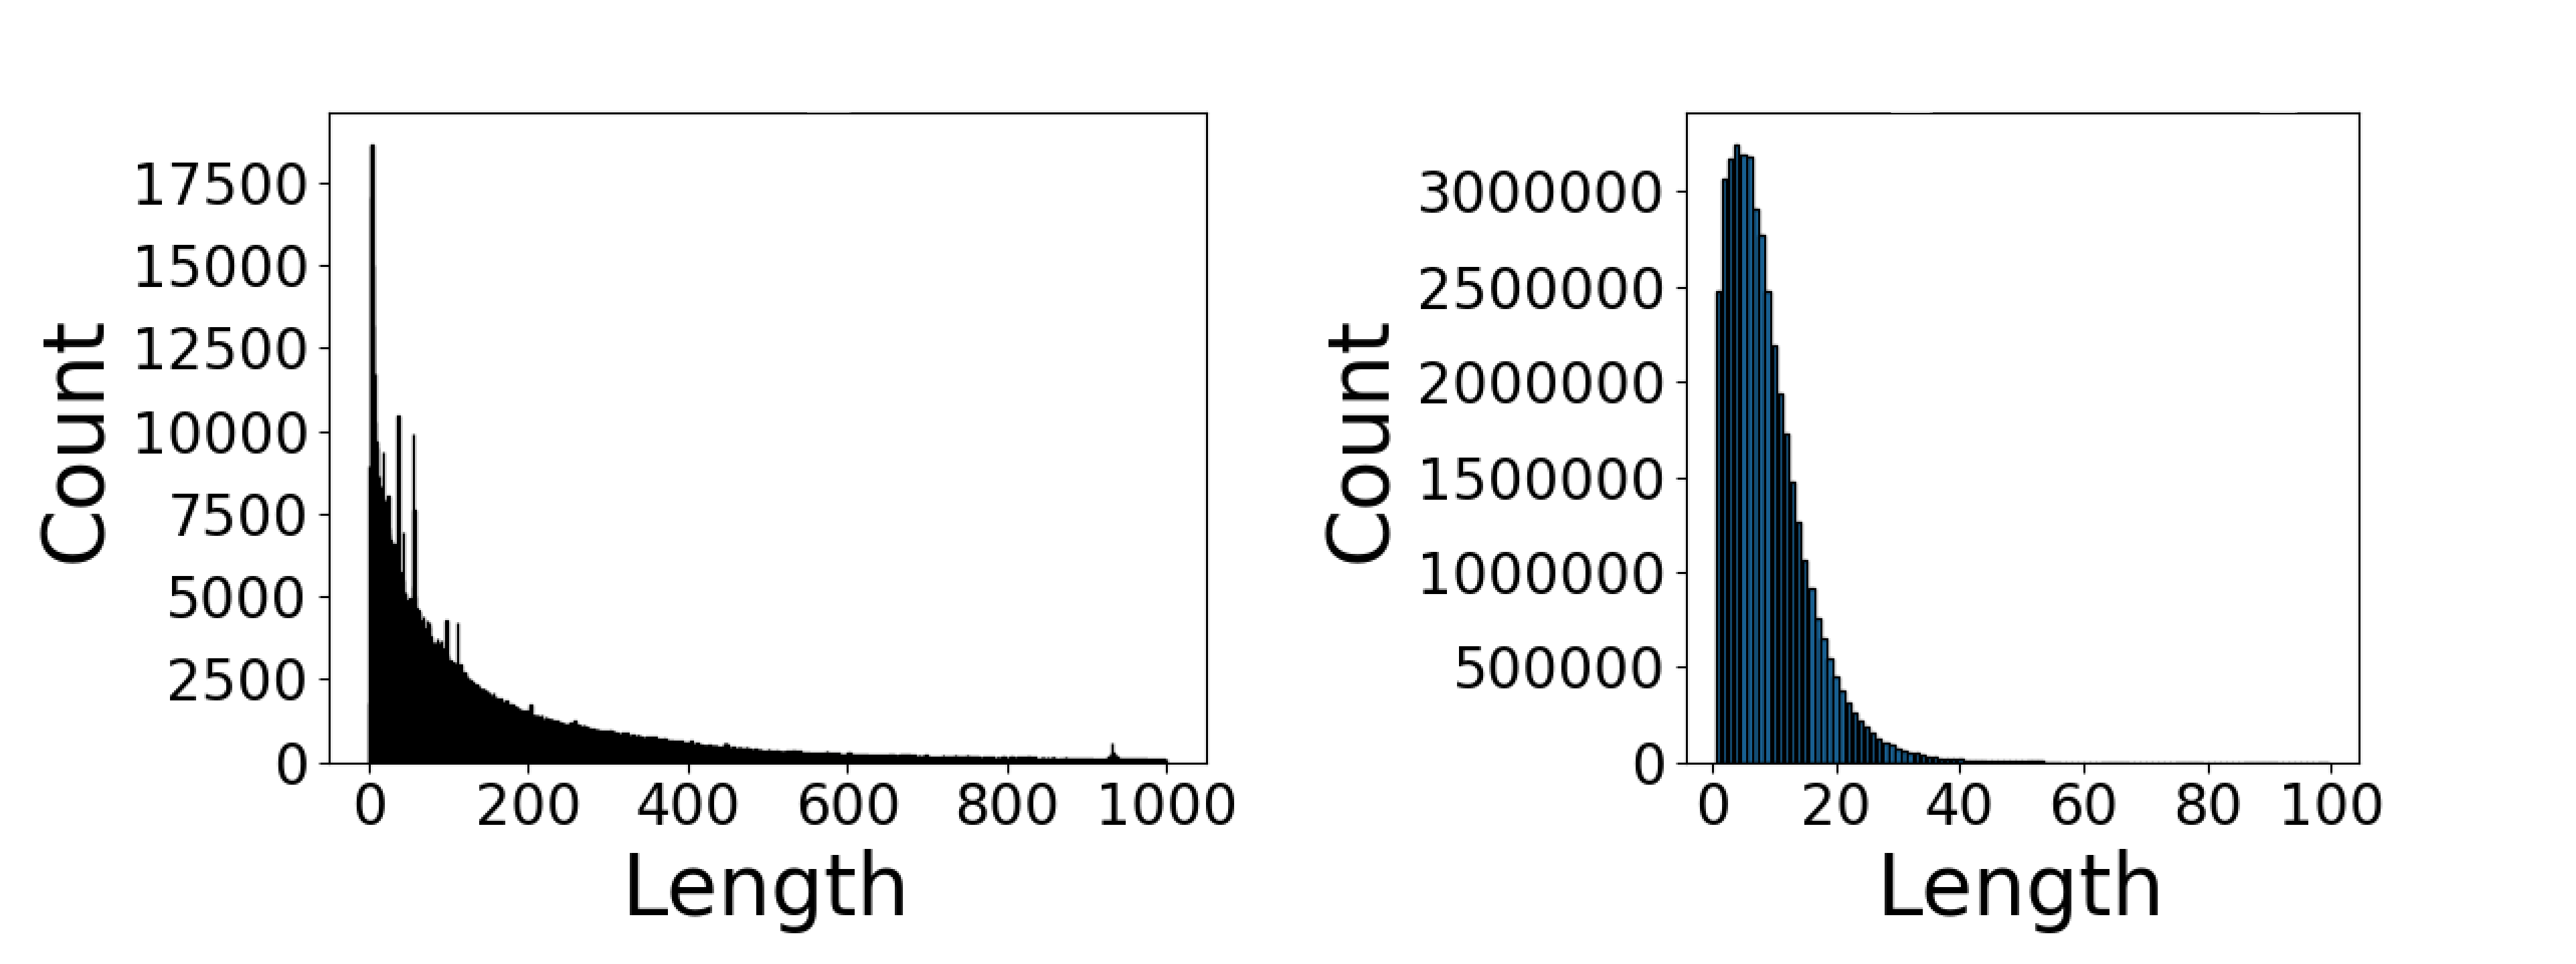
\includegraphics[width=1\textwidth,height=180px]{docLengths}
	\caption{Az 1000 token alatti dokumentumok száma (balra); A 100 token alatti dokumentumok száma (jobbra)}
\end{figure}

\begin{figure}[H]
	\centering
	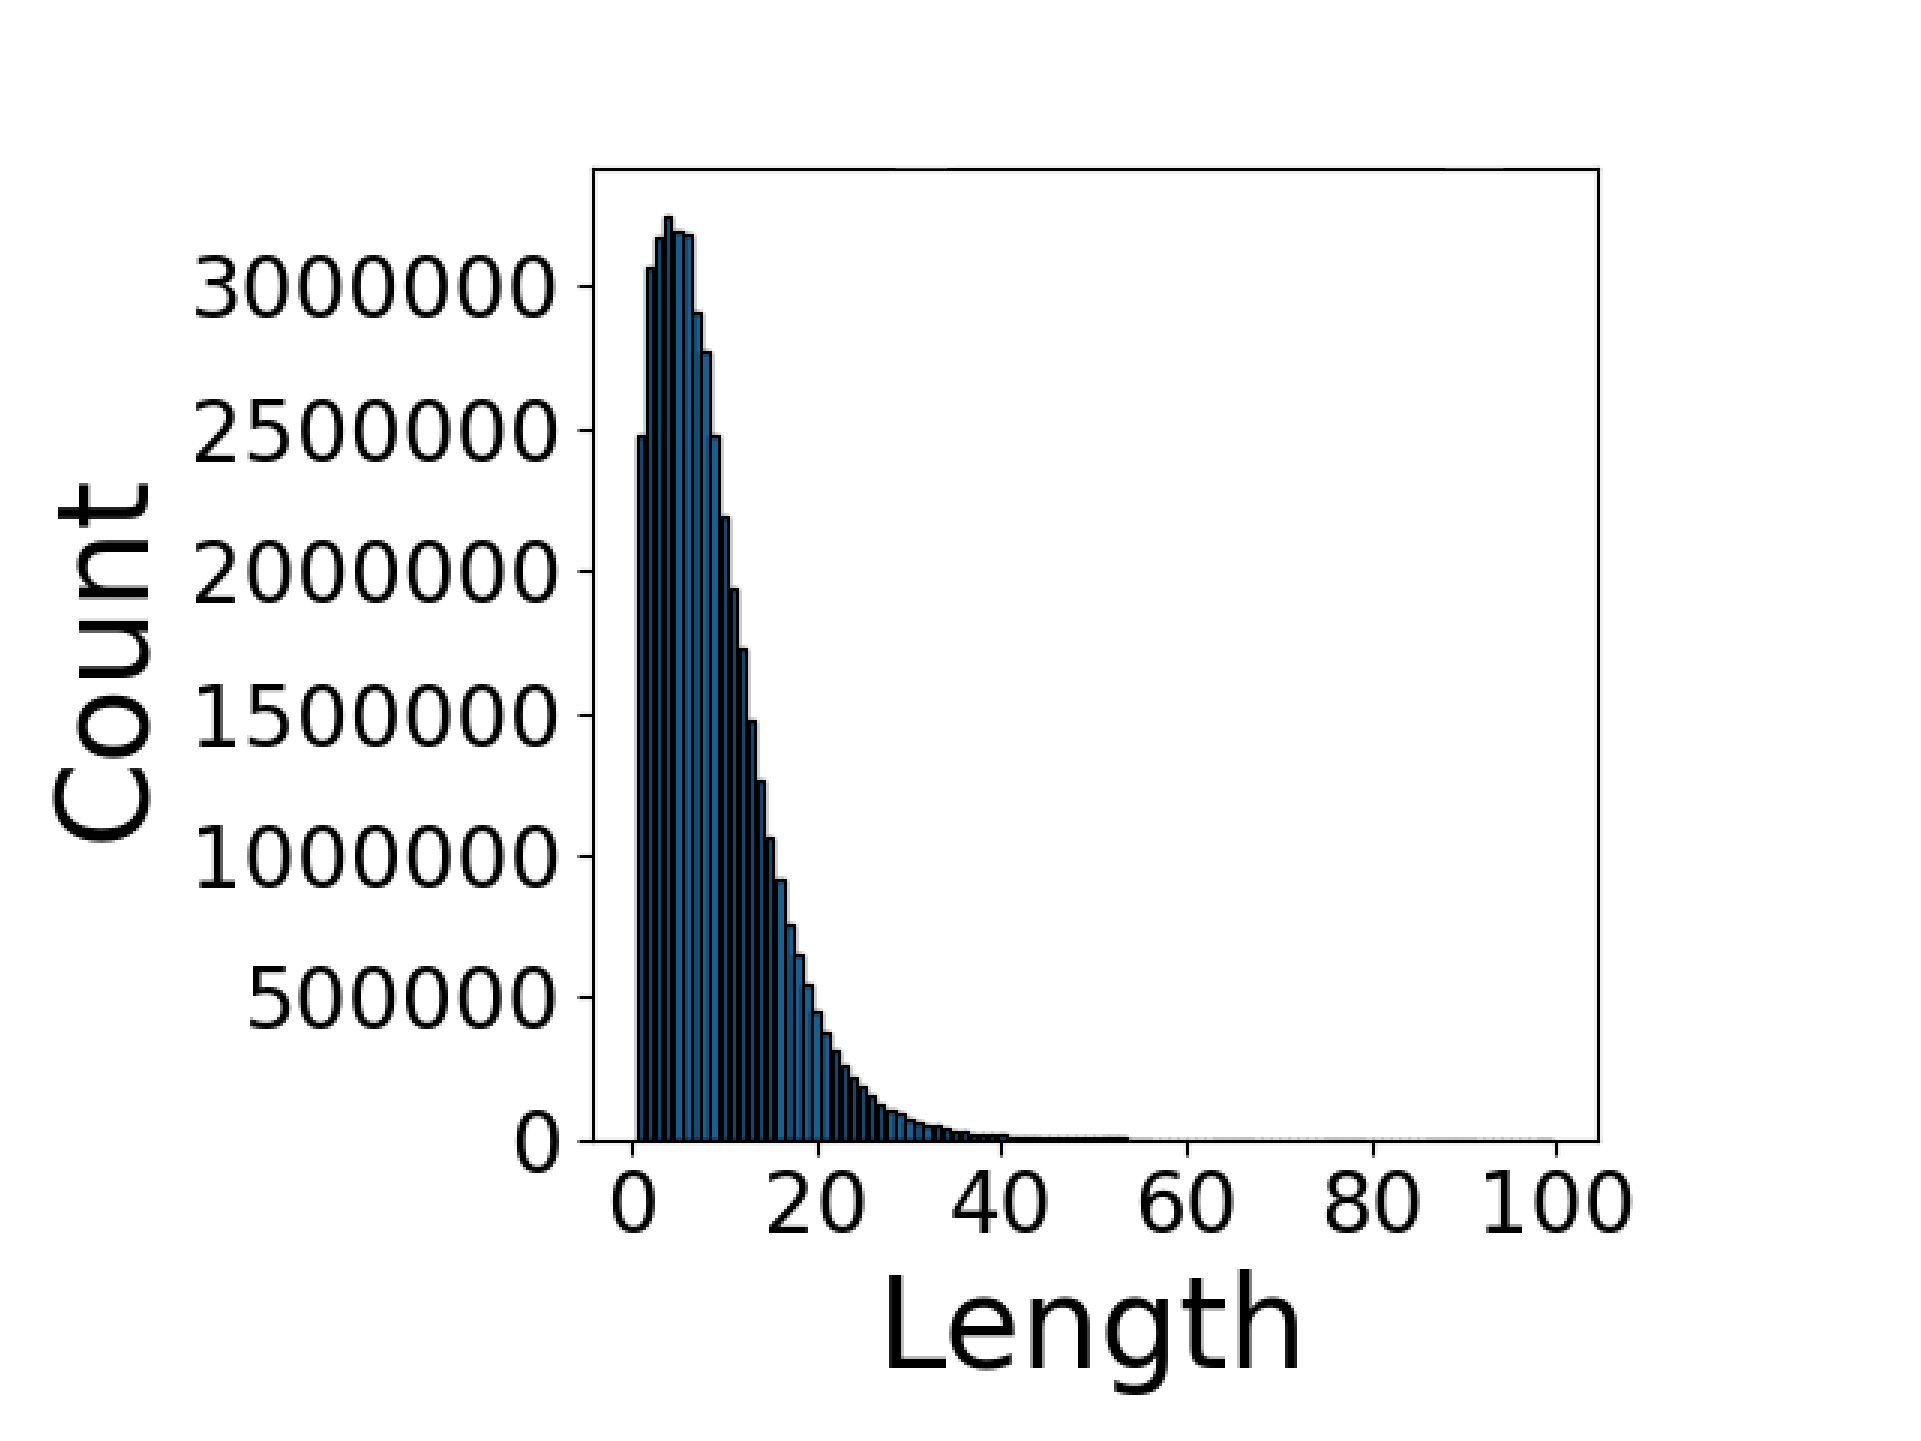
\includegraphics[width=0.6\textwidth,height=180px]{lineLengths}
	\caption{Az 50 token hosszúság alatti mondatok}
\end{figure}

A dokumentumokra és a dokumentumok soraira vonatkozó mérések alapján minimális token-számnak 10-et, maximális szekvenciahossznak 100-at határoztam meg. A cél az volt, hogy a lehető legtöbb információt sikerüljön kinyerni a dokumentumokból és csak relatíve kevés esetben kelljen \textit{padding}-et alkalmazni, továbbá ne legyen a konfigurációnak teljesíthetetlen memóriaigénye. A végső bemeneti hossz így 201 lett.

Bemeneti réteg használata esetén a neurális háló inputjára a mondatpárok token-jeinek Word2Vec azonosítója kerül. Az \textit{embedding lookup} művelet ezen azonosítók segítségével választja ki a réteg számára átadott beágyazási mátrixból az adott token-ekhez tartozó szóvektorokat. Felmerülhet a kérdés, hogy mi történik a speciális token-ekkel ebben az esetben. A speciális token-eket a Word2Vec modell nem ismeri, így azok nem kerültek be a beágyazási mátrixba sem. A probléma megoldására bevezettem a meglévő Word2Vec dimenziók mellé minden egyes speciális token számára egy saját dimenziót és a hozzá tartozó azonosítókat. Ezen token-eket reprezentáló vektorok kiterjedése a saját dimenziójukban 1, az összes többi dimenzióban 0. Így a speciális vektorok merőlegesek a többi vektorra. Ennek okán a speciális token-ek elméletileg nem befolyásolják a tanulás során a szemantikai információkat. A bemeneti rétegnek átadott beágyazási mátrix mérete – az [UNK], Word2Vec modell által nem ismert szavakat jelölő token-nel együtt – $(\text{word\_embedding\_dim} + 4) \times \text{szótár méret} $ lesz.

Bár a \textit{maszkolás} és a \textit{következő mondat} feladatok a \textit{multitask learning} során megosztják egymással a bemeneti réteget és a modellt, a feladatok megoldásához használt fejek és a feladatspecifikus bemenetek különböznek.

\subsection{Maszkolás feladat}

A maszkolási feladat alatt a fej célja kitalálni, milyen token-ek voltak a [MASK] token-ek helyén. A feladat abszolválásához a fejnek szüksége van a mondatpárok generálása során létrejött egyéb információra is. Ilyen információ a maszkolt token-ek szekvencián belüli pozíciója, Word2Vec azonosítója és súlya. Mivel a [MASK] token-ek megfelelő eloszlása érdekében az algoritmus a [PAD] token-eket is letakarja, ezért fontos tényező a súlyok bevezetése. Egy maszkolt token súlya 0 lesz, ha a token eredetileg [PAD] token volt, egyébként 1. 

A fej a BiLSTM háló \textit{pooling} nélküli, szekvenciális kimenetével dolgozik. A kimenetből kiválasztja a maszkolt szavak reprezentációit. Az így kapott \textit{num\_hidden} hosszú vektorokat egy sűrűn kapcsolt, GELU aktivációval \cite{gelu} ellátott rétegen vezeti át, melynek kimeneti mérete megegyezik a kibővített Word2Vec modell beágyazási dimenziójával. Majd a sűrű rétegtől kapott kimenetet megszorozza a beágyazási mátrixszal, annak érdekében, hogy az egyes vektorok a szótár dimenziójába kerüljenek, továbbá \textit{log softmax} aktivációt alkalmaz, hozzájutva a maszkolt token-ekre vonatkozó valószínűségek logaritmusához a teljes szótárra nézve. A feladat tanítási \textit{loss} függvénye az egyes eredeti token-ekre vonatkozó logaritmusok összegének ellentettjének átlaga.


\subsection{Következő mondat feladat}

A \textit{következő mondat} feladat során a fejnek ki kell találnia, hogy A[SEP]B bemenet esetén B szekvencia A rákövetkezője-e. A tanítás során a fej számára biztosítani kell a szekvenciákhoz tartozó címkéket. Ezen címkéket a bemeneti adathalmazt előállító algoritmus generálja. Előfordulhat olyan eset, mikor az algoritmus nem tud az adott dokumentumból A mondat mellé B mondatot választani, mert a dokumentum túl rövid, vagy éppen dokumentumhatárra ért. Ekkor értelemszerűen minden esetben hamis lesz a címkéje az adott bemeneti szekvenciának. Ez a működés kiegyensúlyozatlansági problémához vezethet, melyet az algoritmusban alkalmazott számláló hatékonyan ki tud védeni. Ha többségbe kerül a negatív esetek száma, az algoritmus 1 valószínűséggel pozitív eseteket generál. 

\begin{note}
	A jobb megértés érdekében a dolgozathoz mellékeltem egy példa bemenetet. [\ref{appx:input}]
\end{note}

A fej a BiLSTM háló \textit{max pooling} utáni vektoriális kimenetével, tehát a mondatokat reprezentáló vektorokkal dolgozik. A mondatvektorokra klasszikus bináris klasszifikációt alkalmaz, azaz egy sűrűn kapcsolt rétegen vezeti át őket, melynek kimenete 2 széles és az aktivációs függvénye a \textit{log softmax}. A feladat tanítási \textit{loss} függvénye az így kapott logaritmusok összegének ellentettjének átlaga lesz.

\subsection*{Tanítás - folytatás}
A \textit{multitask learning} során a neurális háló egyszerre két feladatot próbál megoldani, így jobban generalizál. A háló az SGD (\textit{Stochastic Gradient Descent}) nevű algoritmus segítségével minimalizálja a globális \textit{loss} függvényt, amely a két feladat \textit{loss} függvényének összege.
Az SGD számára implementáltam egy konfigurálható \textit{decay} algoritmust. A \textit{learning rate decay} a \textit{loss} függvény értékének \textit{epoch}-onkénti túl lassú csökkenése esetén öttel osztja a \textit{learning rate}-et, így elérve a jobb konvergációs képességet. Az algoritmus minden \textit{epoch} során menti a \textit{transfer} számára szükséges súlyokat és a tanítás aktuális állapotát is.

A jól paraméterezhető tanítás érdekében az implementáció során törekedtem a minél széleskörűbb konfigurálhatóságra. A következő tanításra vonatkozó értékeket állíthatja a felhasználó:
\begin{itemize}
	\item \textit{batch\_size} : A tanításhoz használt \textit{minibatch}-ek mérete.
	\item \textit{num\_inputs} : Az input vektorok mérete.
	\item \textit{num\_time\_steps} : A bemenet szélessége.
	\item \textit{min\_sentence\_length} : A legkisebb token-szám amit az algoritmusnak figyelembe kell vennie.
	\item \textit{max\_sentence\_length} : Az egyes mondatok \textit{padding} utáni hossza.
	\item \textit{masked\_lm\_prob} : A token-ek maszkolási valószínűsége.
	\item \textit{max\_predictions\_per\_seq} : A legnagyobb maszkolható tokenszám egy mondatpár esetén.
	
	\item \textit{learning\_rate\_start} : A \textit{learning rate} kezdőértéke.
	\item \textit{lr\_decay} : \textit{Learning rate decay} ki/be.
	\item \textit{lr\_decay\_threshold} : Az előző és az aktuális \textit{epoch loss} érték mekkora különbsége estén ossza le a \textit{learning rate}-et öttel. Az alapérték 0, tehát ha magasabb, vagy ugyan akkora az aktuális \textit{epoch loss} érték, mint az előző.
	\item \textit{epochs} : Az adathalmazon történő iterációk száma.
	\item \textit{mask\_padding} : Maszkolja-e a \textit{padding} karaktereket.
\end{itemize}

A futtatáshoz használt szervergép konfigurációja a következő: 2 x Intel\textregistered Xeon\textregistered  Processor E5-2640 v4 25M Cache 2.40GHz (10 mag) CPU, 2 x NVIDIA GeForce GTX 1080 Ti GPU, 4 x 32 GB DDR4 RAM.

A neurális modellek kezdeti, teljes adathalmazon történő tanítása \textit{epoch}-onként 4 napot vett volna igénybe, így a generált halmaz méretét a negyedére csökkentettem. Minden modell tanítása esetén 32 méretű \textit{batch}-et és 0.1 kezdeti \textit{learning rate}-et használtam. 

%5 epoch

\section{Vektorok generálása}

A szemantikus reprezentációs vektorok felhasználási területe igen széleskörű. Többek között alkalmazhatóak írott szöveg összegzésére, dokumentumok keresésére, chatbot-ok implementálására, dokumentumok szemantikus hasonlóságának mérésére és szemantikai tartalom szerinti ajánlásra is.

Egy eleve betanított modell mentett súlyainak használata nem igényel komoly erőforrásokat és tárhelyet. A vektorok generálása egy egyszerű folyamat, mely során a reprezentáció fej nélküli neurális hálója – azaz a BiLSTM max pooling – ezen súlyok szerint inicializálásra kerül. Ezt követően a bemenetet a tanításéhoz hasonló módon az input-ra juttatva a neurális modell előállítja a szövegrészletet reprezentáló vektort. A művelet során a háló súlyai nem változnak, azaz képtelen a további tanulásra.

A műveletek elvégzésére elegendő lehet egy CPU is, így a kellő pontosságot elérve a módszer akár ipari rendszerekbe is építhető, vagy különböző webes alkalmazások esetén felhasználói élmény fokozására is felhasználható.


%két kép kicserélése
\cleardoublepage

\chapter{A módszer kiértékelése}
\label{ch:eval}

A modern szemantikus reprezentációs algoritmusok célja, olyan univerzális és általános modellek előállítása, amelyek bármely rendszerben képesek igazodni az adott kihívásokhoz és megfelelő pontossággal teljesíteni az eléjük tűzött feladatokat.

A nyelvi modellek teljesítményének mérése nem triviális feladat. Bár a publikációk során a szerzők többnyire saját módszerrel mérnek, vannak már meglévő komplex kiértékelési keretrendszerek – például SentEval \cite{senteval}, GLUE \cite{glue} – és az igény is egyre nagyobb ezekre. A teljesítmény mérésére szolgáló rendszerek segítségével egységes képet kaphatunk a módszerünk pontosságáról, illetve a csalás lehetősége is korlátozott. A kiértékelés közben a reprezentációs modelleknek olyan feladatok sorozatát kell megoldaniuk, mint a vélemény-polaritás, bináris érzelmi analízis, következtetés vizsgálat, szemantikus hasonlóság.

Mivel a munkám során tanított modellek mindegyike magyar nyelvű, így nem használhattam ezen megoldásokat. Szükségem volt egy saját kiértékelési feladat implementálására.

\section{Árukereső kommentek bináris érzelmi analízise}

Az általam létrehozott modellek pontosságának mérésére használt feladatnak több szempont szerint is meg kellett felelni. Jó kiértékelési feladat az, amelyik kellőképpen "nehéz", így a modellek közti teljesítménybeli különbségek jól interpretálhatóak. Továbbá a feladathoz tartozó adathalmaznak elég elemet kell tartalmaznia ahhoz, hogy a feladat elkerülje a túltanulás problémáját és hiteles eredményt kapjunk végeredményül. Az \textit{arukereso}-nek nevezett adathalmaz bináris osztályozása a kommentek érzelmi tartalma alapján megfelelő kihívásnak minősült ahhoz, hogy az általam tanított modellek pontosságát meg tudjam határozni.

A mérés során az annotált tanítóhalmaz elemeit – azaz pozitív vagy negatív osztályba tartozó kommenteket – a meglévő modellek segítségével vektortérbe képeztem. Majd az így kapott vektor-címke párokkal tanítottam különféle osztályozó algoritmusokat. Ezen algoritmusok teszthalmazon történő kiértékelésének kimenete adta meg az adott szemantikus modell pontosságát.

Szükségem volt egy olyan viszonyítási alapra, amely a már létező magyar nyelvű módszerek teljesítményét szimbolizálja. Erre a célra a kommentek szavait az előre betanított \textit{oscar} és \textit{oscar\_sm} Word2Vec modellekkel leképezve, majd átlagolva megkaptam az adott kommentet reprezentáló 300 hosszú vektorokat.

Mivel a vélemények változó méretűek, továbbá legalább 10 token-ből állnak, a BiLSTM esetén csak az első 201 token került a bemenetre a vektorok generálása során. A túl rövid paragrafusokat a tanításhoz hasonlóan \textit{padding}-eltem.

Egy bináris osztályozási feladat teljesítményét többféle metrika szerint is lehet mérni. Ezek közül a legnépszerűbb a klasszifikációs \textbf{pontosság} (\textit{accuracy}), amely a helyesen prediktált elemek számának és az összes elem számának hányadosa. A \textbf{tévesztési mátrix} (\textit{confusion matrix}) leírja és vizualizálja modellünk teljesítményét az igaz pozitívként, igaz negatívként, hamis pozitívként és hamis negatívként prediktált elemek számának segítségével. A \textbf{vevő működési karakterisztika} (\textit{receiver operating characteristic}) görbe az igaz pozitív és a hamis negatív arányok közötti kapcsolatot vizualizálja. Egy véletlenszerű modell görbéje a főátlón helyezkedik el, ahol y tengelyen az igaz pozitív, x tengelyen a hamis negatív arányok szerepelnek. Minél nagyobb a görbe alatti terület, annál jobb a modellünk performanciája.


\begin{table}[htb]
	\centering
	\begin{tabular}{ | c | r | r | r | r | r | r |}
		\hline
		\multirow{2}{*}{\textbf{Modell / Osztályozó}} & \multirow{2}{*}{\textbf{Linear SVM}} & \multirow{2}{*}{\textbf{XGBoost}} & \multirow{2}{*}{\textbf{Random Forest}} \\
		& & & \\
		\hline \hline		
		\textbf{w2v\_sm} & 85,45\% & 82,18\% & 83,64\% \\
		\hline
		\textbf{w2v\_sm\_norm} & 85,57\% & 82,71\% & \textbf{84,18\%} \\
		\hline
		\textbf{w2v\_lg} & 85,28\% & 82,87\% & 83,77\% \\
		\hline
		\textbf{w2v\_lg\_norm} & \textbf{85,59\%} & 83,15\% & 83,85\% \\
		\hline  
		\textbf{lstm\_1024} & 81,53\% & 80,82\% & 80,84\% \\
		\hline  
		\textbf{lstm\_1024\_norm} & 85,37\% & \textbf{83,48\%} & 83,41\% \\
		\hline  
	\end{tabular}
	\caption[A modellek pontossága]{A modellek klasszifikációs pontossága az arukereso adathalmazon. A w2v\_sm az oscar\_sm, a w2v\_lg az oscar halmazon tanított modelleket, a norm posztfix a normált bemenetet jelöli. A számok a modellek nevében a reprezentációs vektor méretére utalnak.}
	\label{tab:evaluation}
\end{table}

%TODO

%\pagebreak

%-------------------------------------------------------------------------------
% w2v_lg, w2v_lg_normed, w2v_sm, w2v_sm_normed

%saját modellek és részletes leírásaik: lstm_1024, lstm_1024_normed, lstm_4096

%accuracy

%

%hogyan értelmezem?

%befejezés:
%saját halmaz - nem túl kiterjedt, tehát nem a nyelvi modell egészét méri de adott feladatra jó

%más módszereket is ki lehet vele mérni, publikusan elérhető adathalmaz



%arukereso auto annotált/humán annotált?








\cleardoublepage

\chapter{Összegzés} % Conclusion
\label{ch:sum}

A természetes szövegfeldolgozás és annak ágazata, a szemantikus reprezentációk mind akadémiai, mind ipari értelemben gyorsuló ütemben fejlődő területek, amelyek a mai napig rengeteg felderítésre váró lehetőséget tartogatnak. A numerikus ábrázoló algoritmusok teljesítményének növekedése olyan gyakorlati alkalmazások pontosságának javulását indukálják, melyek segítségével hatékonyan kiszűrhető a gyűlöletbeszéd a szociális médiából, vagy akár eredményesen felvehető a harc az álhírek terjedésével szemben. 

Diplomamunkám végeredménye egy kétirányú mondat- és paragrafusszintű előre tanított szemantikus reprezentációs modell, amely képes leképezni a magyar nyelven írt mondatokat a szemantikus térbe.

Magyar nyelvű tanítóadat a nyelv beszéltségéből fakadóan nem, vagy csak elvétve elérhető. A módszer tanításához használt adathalmaz előállítása nem igényel emberi címkézést, olcsó és a végtelenségig skálázható. Továbbá a tanításra szolgáló feladatok jellegéből fakadóan, az algoritmus jó eséllyel átültethető más kis és közepes nyelvre is.

A munkám során több, különféle magyar nyelvű adathalmazt vizsgáltam, melyek akár Word2Vec modellek, akár a bemutatott nyelvi modell létrehozására is alkalmasak lehetnek. Majd konstruáltam egy olyan, a magyar nyelvű szemantikus reprezentációs algoritmusok teljesítményének összehasonlítására használható halmazt, amelyen bináris klasszifikáció végezhető az elemek érzelmi tartalma alapján.
 
A dolgozatban bemutatott modellek tanítása során számos paraméterrel és beállítással próbálkoztam, majd ezek közül a legjobban teljesítő jelöltek teljesítményét a prezentált adathalmaz segítségével kimértem és összehasonlító elemzéseket végeztem.

%TODO: EREDMÉNYEK
interpretálás



\section{Javítási lehetőségek}
A szemantikus reprezentációs módszerekben rejlő lehetőségek a mai napig ismeretlenek és feltérképezetlenek. A tanulás vagy vektorgenerálás során optimalizált paraméterbeállítások és kombinációk további teljesítménybeli javulást hozhatnak.

A jövőben érdemes lehet az SGD helyett más optimalizáló algoritmust választani, továbbá a mélyhálóban alkalmazott \textit{max pooling}-ot \textit{mean pooling}-ra cserélni.

A megfigyelések alapján a GloVe szóbeágyazási módszer jobb eredményeket ér el, mint a Word2Vec, így célravezető lehet a beágyazási rétegben GloVe-ot használni.

Bizonyos esetekben a mélyebb architektúrák hatékonyabban tudják kinyerni a szekvenciális szöveges adatokból származó információkat, így több egymásra illesztett BiLSTM, vagy akár BiGRU réteg együttes tanítása pontosabb végeredményhez vezethet.

Az általam létrehozott nyelvi modellek mindegyike előtanított, finomhangolást nem végeztem rajtuk. A \textit{transfer learning} segítségével finomhangolt modellek több esetben jelentősen jobban teljesítenek, továbbá adatigényük is kisebb az előtanításénál. A jövőben a meglévő neurális modelleket egy olyan feladattal tervezem tovább tanítani, amelyben a háló célja egy értelmező kéziszótárból kinyert cikkek alapján kitalálni a cikkekhez tartozó szót.

Jelen működés szerint a maszkolt szavak közül csak a \textit{padding} token-ek kerülnek 0 súllyal a bemenetre. Ha sok ismeretlen szó található a tanítási halmazban, akkor a modellünk elfogulttá válhat az ismeretlen szavakat reprezentáló token felé, így nehezebbé téve a tanulási folyamatot. Ennélfogva előfordulhat, hogy az ilyen token-ek nullával való súlyozása jobb konvergációra készteti a modellt.

\chapter*{Összegzés - folytatás}

\section{Köszönetnyilvánítás}

magyar NLP ezen ágát egy kicsit katalizálja; az előtanítási módszereket és a benchmarkot is fel tudják használni és tovább tanítani

köszönet
\cleardoublepage

% Függelékek (opcionális) - hosszabb részletező táblázatok, sok és/vagy nagy kép esetén hasznos
% Appendices (optional) - useful for detailed information in long tables, many and/or large figures, etc.
\appendix
\chapter{Példa bemenet}
\label{appx:input}

\textbf{tokens - bemeneti token-ek:}
szerény termékeny magyar filmipar meglepő film tűni többnyire szociális probléma dráma foglalkozik műv színvonal átlag felüli tűni magyar filmgyártás [MASK] ambíció mozi hoz lét magyar filmkészítő megbecsül külföld [MASK] kései fejlődés magyarország film viszony késő tör stúdió jön lét mindkettő [MASK] indúlt fejlődés kezdetben irodalmi mű dolgozik [MASK] lévő osztrák magyar monarchia égisz es kommunista vezetés [MASK] [MASK] meglepő mód hónapos uralom film készül [MASK] kommunista uralom összeomlás horty kapillaritás [MASK] [MASK] kiemelkedő tehetség hagy [MASK] időszak kertész mihály michael curtiz fejős pál paul fejos balázs béla peter [MASK] lugosi [MASK] lukács pál paul [MASK] [MASK] év terroruralom honi filmgyártás [SEP] mély álom sűllyedt as [MASK] év német befolyás [MASK] felűlmúlta propaganda mennyiség napi parancs háború utáni neorealista mozgalom magyar kifejezésmód csodaszép alkotás devizaátutalás maga valahol európa amely árva [MASK] szenvedés keresztűl mutat háború pusztítás felnőtt okoz elítélnék borzalom önfejű tesz kommunista államosít filmipar ideológiai [MASK] lát szociális probla foglalkozó film [MASK] hazai filmgyártás eredmény virágzó filmipar [MASK] propaganda jellemez hullám as belezsúfolni rendezők [MASK] képes kialakít nyelvezet [MASK] képi szimbólum nemzeti téma ültet alkotás francia hullám eltérő magyar utasít próbál eltér hagyomány mag [MASK] rendezők kézdi kovács sándor pál sajátos stílus alakít mozi [MASK] állam elkötelezett filmfesztivál elért eredmény [MASK]

\textbf{input\_ids - bemeneti W2V azonosítók:}
5382 12900 2 37008 2156 95 33811 2388 503 175 3356 561 7814 2660 2184 7771 33811 2 33898 645137 15313 1521 157 557 2 40114 14740 1413 645137 16398 769 125 95 1321 3408 1890 2110 97 557 3391 645137 234617 769 7873 1930 799 220 645137 246 2188 2 8201 24238 498151 3877 946 645137 645137 2156 76 2825 5559 95 287 645137 3877 5559 10192 271054 628178 645137 645137 1481 2518 251 645137 420 5560 1075 4142 232007 59044 1002 6207 645139 1142 1111 6077 645137 35671 645137 5265 1002 6207 645137 645137 1 569799 19546 33898 645138 710 1182 645139 357 645137 1 259 5069 645137 534521 6988 743 453 3182 1216 1555 387909 2411 2 48872 9266 1074 586461 645139 2413 297 645139 9402 645137 3310 54345 154 1216 9095 625 530 645139 14327 40193 11 3877 43443 37008 11581 645137 45 503 645139 1923 95 645137 423 33898 137 9693 37008 645137 6988 2639 3143 357 588735 54795 645137 231 4395 14592 645137 4026 3558 122 230 5189 1074 701 3143 1203 2 6365 375 4907 1190 486 645137 54795 63938 1004 477 1002 2668 933 1373 1521 645137 730 4695 8935 3109 137 645137

\textbf{masked\_lm\_ids - maszkolt szavak azonosítói:}
12941 20703 726 150472 37008 43443 13246 271054 31 13246 18991 86 222962 1111 46797 357 498151 556 387909 74 104 3914 11009 1074 1 1935 526 1324 171 645

\textbf{masked\_lm\_weights - maszkolt szavak súlyai:}
1 1 1 1 1 1 1 1 1 1 1 1 1 1 1 1 1 1 1 1 1 1 1 1 1 1 1 1 1 1

\textbf{masked\_lm\_positions - maszkolt szavak pozíciói:}
19 28 40 47 56 57 64 68 69 70 71 75 88 90 94 95 105 109 117 123 129 145 151 157 162 164 168 184 194 200

\textbf{sentence\_labels - következő mondat címke:}
1

%\cleardoublepage

% Irodalomjegyzék (kötelező)
% Bibliography (mandatory)
\addcontentsline{toc}{chapter}{\biblabel}
\printbibliography[title=\biblabel]
\cleardoublepage

% Ábrajegyzék (opcionális) - 3-5 ábra fölött érdemes
% List of figures (optional) - useful over 3-5 figures
\addcontentsline{toc}{chapter}{\lstfigurelabel}
\listoffigures
\cleardoublepage

% Táblázatjegyzék (opcionális) - 3-5 táblázat fölött érdemes
% List of tables (optional) - useful over 3-5 tables
%\addcontentsline{toc}{chapter}{\lsttablelabel}
%\listoftables
%\cleardoublepage

% Forráskódjegyzék (opcionális) - 3-5 kódpélda fölött érdemes
% List of codes (optional) - useful over 3-5 code samples
%\addcontentsline{toc}{chapter}{\lstcodelabel}
%\lstlistoflistings
%\cleardoublepage

% Jelölésjegyzék (opcionális)
% List of symbols (optional)
%\printnomenclature

\end{document}
